\documentclass[twoside]{book}

% Packages required by doxygen
\usepackage{fixltx2e}
\usepackage{calc}
\usepackage{doxygen}
\usepackage[export]{adjustbox} % also loads graphicx
\usepackage{graphicx}
\usepackage[utf8]{inputenc}
\usepackage{makeidx}
\usepackage{multicol}
\usepackage{multirow}
\PassOptionsToPackage{warn}{textcomp}
\usepackage{textcomp}
\usepackage[nointegrals]{wasysym}
\usepackage[table]{xcolor}

% Font selection
\usepackage[T1]{fontenc}
\usepackage[scaled=.90]{helvet}
\usepackage{courier}
\usepackage{amssymb}
\usepackage{sectsty}
\renewcommand{\familydefault}{\sfdefault}
\allsectionsfont{%
  \fontseries{bc}\selectfont%
  \color{darkgray}%
}
\renewcommand{\DoxyLabelFont}{%
  \fontseries{bc}\selectfont%
  \color{darkgray}%
}
\newcommand{\+}{\discretionary{\mbox{\scriptsize$\hookleftarrow$}}{}{}}

% Page & text layout
\usepackage{geometry}
\geometry{%
  a4paper,%
  top=2.5cm,%
  bottom=2.5cm,%
  left=2.5cm,%
  right=2.5cm%
}
\tolerance=750
\hfuzz=15pt
\hbadness=750
\setlength{\emergencystretch}{15pt}
\setlength{\parindent}{0cm}
\setlength{\parskip}{3ex plus 2ex minus 2ex}
\makeatletter
\renewcommand{\paragraph}{%
  \@startsection{paragraph}{4}{0ex}{-1.0ex}{1.0ex}{%
    \normalfont\normalsize\bfseries\SS@parafont%
  }%
}
\renewcommand{\subparagraph}{%
  \@startsection{subparagraph}{5}{0ex}{-1.0ex}{1.0ex}{%
    \normalfont\normalsize\bfseries\SS@subparafont%
  }%
}
\makeatother

% Headers & footers
\usepackage{fancyhdr}
\pagestyle{fancyplain}
\fancyhead[LE]{\fancyplain{}{\bfseries\thepage}}
\fancyhead[CE]{\fancyplain{}{}}
\fancyhead[RE]{\fancyplain{}{\bfseries\leftmark}}
\fancyhead[LO]{\fancyplain{}{\bfseries\rightmark}}
\fancyhead[CO]{\fancyplain{}{}}
\fancyhead[RO]{\fancyplain{}{\bfseries\thepage}}
\fancyfoot[LE]{\fancyplain{}{}}
\fancyfoot[CE]{\fancyplain{}{}}
\fancyfoot[RE]{\fancyplain{}{\bfseries\scriptsize Generated by Doxygen }}
\fancyfoot[LO]{\fancyplain{}{\bfseries\scriptsize Generated by Doxygen }}
\fancyfoot[CO]{\fancyplain{}{}}
\fancyfoot[RO]{\fancyplain{}{}}
\renewcommand{\footrulewidth}{0.4pt}
\renewcommand{\chaptermark}[1]{%
  \markboth{#1}{}%
}
\renewcommand{\sectionmark}[1]{%
  \markright{\thesection\ #1}%
}

% Indices & bibliography
\usepackage{natbib}
\usepackage[titles]{tocloft}
\setcounter{tocdepth}{3}
\setcounter{secnumdepth}{5}
\makeindex

% Hyperlinks (required, but should be loaded last)
\usepackage{ifpdf}
\ifpdf
  \usepackage[pdftex,pagebackref=true]{hyperref}
\else
  \usepackage[ps2pdf,pagebackref=true]{hyperref}
\fi
\hypersetup{%
  colorlinks=true,%
  linkcolor=blue,%
  citecolor=blue,%
  unicode%
}

% Custom commands
\newcommand{\clearemptydoublepage}{%
  \newpage{\pagestyle{empty}\cleardoublepage}%
}

\usepackage{caption}
\captionsetup{labelsep=space,justification=centering,font={bf},singlelinecheck=off,skip=4pt,position=top}

%===== C O N T E N T S =====

\begin{document}

% Titlepage & ToC
\hypersetup{pageanchor=false,
             bookmarksnumbered=true,
             pdfencoding=unicode
            }
\pagenumbering{alph}
\begin{titlepage}
\vspace*{7cm}
\begin{center}%
{\Large \mbox{[}H\+PC\mbox{]} Simulation process ans Data Management Tool }\\
\vspace*{1cm}
{\large Generated by Doxygen 1.8.13}\\
\end{center}
\end{titlepage}
\clearemptydoublepage
\pagenumbering{roman}
\tableofcontents
\clearemptydoublepage
\pagenumbering{arabic}
\hypersetup{pageanchor=true}

%--- Begin generated contents ---
\chapter{Hierarchical Index}
\section{Class Hierarchy}
This inheritance list is sorted roughly, but not completely, alphabetically\+:\begin{DoxyCompactList}
\item \contentsline{section}{S\+D\+MT\+:\+:Ckpt\+Info}{\pageref{struct_s_d_m_t_1_1_ckpt_info}}{}
\item \contentsline{section}{S\+D\+MT\+:\+:Config}{\pageref{struct_s_d_m_t_1_1_config}}{}
\item \contentsline{section}{tinyxml2\+:\+:Dyn\+Array$<$ T, I\+N\+I\+T\+I\+A\+L\+\_\+\+S\+I\+ZE $>$}{\pageref{classtinyxml2_1_1_dyn_array}}{}
\item \contentsline{section}{tinyxml2\+:\+:Dyn\+Array$<$ Block $\ast$, 10 $>$}{\pageref{classtinyxml2_1_1_dyn_array}}{}
\item \contentsline{section}{tinyxml2\+:\+:Dyn\+Array$<$ char, 20 $>$}{\pageref{classtinyxml2_1_1_dyn_array}}{}
\item \contentsline{section}{tinyxml2\+:\+:Dyn\+Array$<$ const char $\ast$, 10 $>$}{\pageref{classtinyxml2_1_1_dyn_array}}{}
\item \contentsline{section}{tinyxml2\+:\+:Dyn\+Array$<$ tinyxml2\+:\+:X\+M\+L\+Node $\ast$, 10 $>$}{\pageref{classtinyxml2_1_1_dyn_array}}{}
\item \contentsline{section}{tinyxml2\+:\+:Entity}{\pageref{structtinyxml2_1_1_entity}}{}
\item \contentsline{section}{serialize\+:\+:I}{\pageref{classserialize_1_1_i}}{}
\item \contentsline{section}{tinyxml2\+:\+:Long\+Fits\+Into\+Size\+T\+Minus\+One$<$ bool $>$}{\pageref{structtinyxml2_1_1_long_fits_into_size_t_minus_one}}{}
\item \contentsline{section}{tinyxml2\+:\+:Long\+Fits\+Into\+Size\+T\+Minus\+One$<$ false $>$}{\pageref{structtinyxml2_1_1_long_fits_into_size_t_minus_one_3_01false_01_4}}{}
\item \contentsline{section}{tinyxml2\+:\+:Mem\+Pool}{\pageref{classtinyxml2_1_1_mem_pool}}{}
\begin{DoxyCompactList}
\item \contentsline{section}{tinyxml2\+:\+:Mem\+PoolT$<$ sizeof(tinyxml2\+:\+:X\+M\+L\+Attribute) $>$}{\pageref{classtinyxml2_1_1_mem_pool_t}}{}
\item \contentsline{section}{tinyxml2\+:\+:Mem\+PoolT$<$ sizeof(tinyxml2\+:\+:X\+M\+L\+Comment) $>$}{\pageref{classtinyxml2_1_1_mem_pool_t}}{}
\item \contentsline{section}{tinyxml2\+:\+:Mem\+PoolT$<$ sizeof(tinyxml2\+:\+:X\+M\+L\+Element) $>$}{\pageref{classtinyxml2_1_1_mem_pool_t}}{}
\item \contentsline{section}{tinyxml2\+:\+:Mem\+PoolT$<$ sizeof(tinyxml2\+:\+:X\+M\+L\+Text) $>$}{\pageref{classtinyxml2_1_1_mem_pool_t}}{}
\item \contentsline{section}{tinyxml2\+:\+:Mem\+PoolT$<$ I\+T\+E\+M\+\_\+\+S\+I\+ZE $>$}{\pageref{classtinyxml2_1_1_mem_pool_t}}{}
\end{DoxyCompactList}
\item \contentsline{section}{S\+D\+MT}{\pageref{class_s_d_m_t}}{}
\item \contentsline{section}{S\+D\+MT\+:\+:Segment}{\pageref{struct_s_d_m_t_1_1_segment}}{}
\item \contentsline{section}{serialize}{\pageref{classserialize}}{}
\item \contentsline{section}{tinyxml2\+:\+:Str\+Pair}{\pageref{classtinyxml2_1_1_str_pair}}{}
\item \contentsline{section}{tinyxml2\+:\+:X\+M\+L\+Attribute}{\pageref{classtinyxml2_1_1_x_m_l_attribute}}{}
\item \contentsline{section}{tinyxml2\+:\+:X\+M\+L\+Const\+Handle}{\pageref{classtinyxml2_1_1_x_m_l_const_handle}}{}
\item \contentsline{section}{tinyxml2\+:\+:X\+M\+L\+Handle}{\pageref{classtinyxml2_1_1_x_m_l_handle}}{}
\item \contentsline{section}{tinyxml2\+:\+:X\+M\+L\+Node}{\pageref{classtinyxml2_1_1_x_m_l_node}}{}
\begin{DoxyCompactList}
\item \contentsline{section}{tinyxml2\+:\+:X\+M\+L\+Comment}{\pageref{classtinyxml2_1_1_x_m_l_comment}}{}
\item \contentsline{section}{tinyxml2\+:\+:X\+M\+L\+Declaration}{\pageref{classtinyxml2_1_1_x_m_l_declaration}}{}
\item \contentsline{section}{tinyxml2\+:\+:X\+M\+L\+Document}{\pageref{classtinyxml2_1_1_x_m_l_document}}{}
\item \contentsline{section}{tinyxml2\+:\+:X\+M\+L\+Element}{\pageref{classtinyxml2_1_1_x_m_l_element}}{}
\item \contentsline{section}{tinyxml2\+:\+:X\+M\+L\+Text}{\pageref{classtinyxml2_1_1_x_m_l_text}}{}
\item \contentsline{section}{tinyxml2\+:\+:X\+M\+L\+Unknown}{\pageref{classtinyxml2_1_1_x_m_l_unknown}}{}
\end{DoxyCompactList}
\item \contentsline{section}{tinyxml2\+:\+:X\+M\+L\+Util}{\pageref{classtinyxml2_1_1_x_m_l_util}}{}
\item \contentsline{section}{tinyxml2\+:\+:X\+M\+L\+Visitor}{\pageref{classtinyxml2_1_1_x_m_l_visitor}}{}
\begin{DoxyCompactList}
\item \contentsline{section}{tinyxml2\+:\+:X\+M\+L\+Printer}{\pageref{classtinyxml2_1_1_x_m_l_printer}}{}
\end{DoxyCompactList}
\end{DoxyCompactList}

\chapter{Class Index}
\section{Class List}
Here are the classes, structs, unions and interfaces with brief descriptions\+:\begin{DoxyCompactList}
\item\contentsline{section}{\hyperlink{struct_s_d_m_t_1_1_ckpt_info}{S\+D\+M\+T\+::\+Ckpt\+Info} \\*Checkpoint info }{\pageref{struct_s_d_m_t_1_1_ckpt_info}}{}
\item\contentsline{section}{\hyperlink{class_s_d_m_t}{S\+D\+MT} \\*Singleton class that provides A\+P\+Is of \hyperlink{class_s_d_m_t}{S\+D\+MT} }{\pageref{class_s_d_m_t}}{}
\item\contentsline{section}{\hyperlink{struct_s_d_m_t_1_1_segment}{S\+D\+M\+T\+::\+Segment} \\*Chunk of memory which is the unit of allocation and management }{\pageref{struct_s_d_m_t_1_1_segment}}{}
\end{DoxyCompactList}

\chapter{Class Documentation}
\hypertarget{struct_s_d_m_t_1_1_ckpt_info}{}\section{S\+D\+MT\+:\+:Ckpt\+Info Struct Reference}
\label{struct_s_d_m_t_1_1_ckpt_info}\index{S\+D\+M\+T\+::\+Ckpt\+Info@{S\+D\+M\+T\+::\+Ckpt\+Info}}


checkpoint info  




{\ttfamily \#include $<$sdmt.\+h$>$}

\subsection*{Public Member Functions}
\begin{DoxyCompactItemize}
\item 
\mbox{\Hypertarget{struct_s_d_m_t_1_1_ckpt_info_a2556be85ca8c498984a94f9e4631ee9a}\label{struct_s_d_m_t_1_1_ckpt_info_a2556be85ca8c498984a94f9e4631ee9a}} 
\hyperlink{struct_s_d_m_t_1_1_ckpt_info_a2556be85ca8c498984a94f9e4631ee9a}{Ckpt\+Info} (int id\+\_\+, int level\+\_\+)
\begin{DoxyCompactList}\small\item\em \hyperlink{struct_s_d_m_t_1_1_ckpt_info}{Ckpt\+Info} constructor. \end{DoxyCompactList}\end{DoxyCompactItemize}
\subsection*{Public Attributes}
\begin{DoxyCompactItemize}
\item 
\mbox{\Hypertarget{struct_s_d_m_t_1_1_ckpt_info_aeb67008d2f1294435c1a07a22ad691ff}\label{struct_s_d_m_t_1_1_ckpt_info_aeb67008d2f1294435c1a07a22ad691ff}} 
int \hyperlink{struct_s_d_m_t_1_1_ckpt_info_aeb67008d2f1294435c1a07a22ad691ff}{id}
\begin{DoxyCompactList}\small\item\em checkpoint id \end{DoxyCompactList}\item 
\mbox{\Hypertarget{struct_s_d_m_t_1_1_ckpt_info_a552a2b7a4cb67498389e41b9dbc93a87}\label{struct_s_d_m_t_1_1_ckpt_info_a552a2b7a4cb67498389e41b9dbc93a87}} 
int \hyperlink{struct_s_d_m_t_1_1_ckpt_info_a552a2b7a4cb67498389e41b9dbc93a87}{level}
\begin{DoxyCompactList}\small\item\em checkpoint level \end{DoxyCompactList}\end{DoxyCompactItemize}


\subsection{Detailed Description}
checkpoint info 

The documentation for this struct was generated from the following file\+:\begin{DoxyCompactItemize}
\item 
/home/ijlee/workspace/sdmt/src/sdmt.\+h\end{DoxyCompactItemize}

\hypertarget{struct_s_d_m_t_1_1_config}{}\section{S\+D\+MT\+:\+:Config Struct Reference}
\label{struct_s_d_m_t_1_1_config}\index{S\+D\+M\+T\+::\+Config@{S\+D\+M\+T\+::\+Config}}


configurations  




{\ttfamily \#include $<$sdmt.\+h$>$}

\subsection*{Public Attributes}
\begin{DoxyCompactItemize}
\item 
\mbox{\Hypertarget{struct_s_d_m_t_1_1_config_a15ac2d93f153f5c3c3b557eb242bf43f}\label{struct_s_d_m_t_1_1_config_a15ac2d93f153f5c3c3b557eb242bf43f}} 
std\+::string \hyperlink{struct_s_d_m_t_1_1_config_a15ac2d93f153f5c3c3b557eb242bf43f}{m\+\_\+archive}
\begin{DoxyCompactList}\small\item\em path to archive sdmt manager \end{DoxyCompactList}\item 
\mbox{\Hypertarget{struct_s_d_m_t_1_1_config_a1508b4a0a71a7d172e3fb5834bd405a8}\label{struct_s_d_m_t_1_1_config_a1508b4a0a71a7d172e3fb5834bd405a8}} 
std\+::string \hyperlink{struct_s_d_m_t_1_1_config_a1508b4a0a71a7d172e3fb5834bd405a8}{m\+\_\+fti\+\_\+config}
\begin{DoxyCompactList}\small\item\em path to fti lib configuration file \end{DoxyCompactList}\end{DoxyCompactItemize}


\subsection{Detailed Description}
configurations 

The documentation for this struct was generated from the following file\+:\begin{DoxyCompactItemize}
\item 
/home/ijlee/workspace/sdmt/src/sdmt.\+h\end{DoxyCompactItemize}

\hypertarget{classtinyxml2_1_1_dyn_array}{}\section{tinyxml2\+:\+:Dyn\+Array$<$ T, I\+N\+I\+T\+I\+A\+L\+\_\+\+S\+I\+ZE $>$ Class Template Reference}
\label{classtinyxml2_1_1_dyn_array}\index{tinyxml2\+::\+Dyn\+Array$<$ T, I\+N\+I\+T\+I\+A\+L\+\_\+\+S\+I\+Z\+E $>$@{tinyxml2\+::\+Dyn\+Array$<$ T, I\+N\+I\+T\+I\+A\+L\+\_\+\+S\+I\+Z\+E $>$}}
\subsection*{Public Member Functions}
\begin{DoxyCompactItemize}
\item 
\mbox{\Hypertarget{classtinyxml2_1_1_dyn_array_af87a804cd831226d069274b44b74b8bc}\label{classtinyxml2_1_1_dyn_array_af87a804cd831226d069274b44b74b8bc}} 
void {\bfseries Clear} ()
\item 
\mbox{\Hypertarget{classtinyxml2_1_1_dyn_array_aea7ffe983b5d3284bd43171afd7c99d0}\label{classtinyxml2_1_1_dyn_array_aea7ffe983b5d3284bd43171afd7c99d0}} 
void {\bfseries Push} (T t)
\item 
\mbox{\Hypertarget{classtinyxml2_1_1_dyn_array_ad289abee8cd02b26e215f1b63d2043f1}\label{classtinyxml2_1_1_dyn_array_ad289abee8cd02b26e215f1b63d2043f1}} 
T $\ast$ {\bfseries Push\+Arr} (int count)
\item 
\mbox{\Hypertarget{classtinyxml2_1_1_dyn_array_a27a3f2f6f869815b6eabb3ea40cf0712}\label{classtinyxml2_1_1_dyn_array_a27a3f2f6f869815b6eabb3ea40cf0712}} 
T {\bfseries Pop} ()
\item 
\mbox{\Hypertarget{classtinyxml2_1_1_dyn_array_ab8b8c94a2312ab27e2846f0d61ef677a}\label{classtinyxml2_1_1_dyn_array_ab8b8c94a2312ab27e2846f0d61ef677a}} 
void {\bfseries Pop\+Arr} (int count)
\item 
\mbox{\Hypertarget{classtinyxml2_1_1_dyn_array_a044fc26f44ed3e96ffaeac542188149e}\label{classtinyxml2_1_1_dyn_array_a044fc26f44ed3e96ffaeac542188149e}} 
bool {\bfseries Empty} () const
\item 
\mbox{\Hypertarget{classtinyxml2_1_1_dyn_array_a756cf4e7464c711aa720e2b17a251daa}\label{classtinyxml2_1_1_dyn_array_a756cf4e7464c711aa720e2b17a251daa}} 
T \& {\bfseries operator\mbox{[}$\,$\mbox{]}} (int i)
\item 
\mbox{\Hypertarget{classtinyxml2_1_1_dyn_array_a474a5cd9bc97ea32b3dcef4c773125e1}\label{classtinyxml2_1_1_dyn_array_a474a5cd9bc97ea32b3dcef4c773125e1}} 
const T \& {\bfseries operator\mbox{[}$\,$\mbox{]}} (int i) const
\item 
\mbox{\Hypertarget{classtinyxml2_1_1_dyn_array_a5e4e1e408e646688503dec77c77c9d59}\label{classtinyxml2_1_1_dyn_array_a5e4e1e408e646688503dec77c77c9d59}} 
const T \& {\bfseries Peek\+Top} () const
\item 
\mbox{\Hypertarget{classtinyxml2_1_1_dyn_array_a67614d80847eb92cab330f1a5849a9a2}\label{classtinyxml2_1_1_dyn_array_a67614d80847eb92cab330f1a5849a9a2}} 
int {\bfseries Size} () const
\item 
\mbox{\Hypertarget{classtinyxml2_1_1_dyn_array_a8e101fdf5b4248ac119d7dca6d0f5421}\label{classtinyxml2_1_1_dyn_array_a8e101fdf5b4248ac119d7dca6d0f5421}} 
int {\bfseries Capacity} () const
\item 
\mbox{\Hypertarget{classtinyxml2_1_1_dyn_array_aa72c644f8b5e9ec5dab5b66c88f5665f}\label{classtinyxml2_1_1_dyn_array_aa72c644f8b5e9ec5dab5b66c88f5665f}} 
void {\bfseries Swap\+Remove} (int i)
\item 
\mbox{\Hypertarget{classtinyxml2_1_1_dyn_array_a60b33e61cf10b3fd900ee46692dc0fe9}\label{classtinyxml2_1_1_dyn_array_a60b33e61cf10b3fd900ee46692dc0fe9}} 
const T $\ast$ {\bfseries Mem} () const
\item 
\mbox{\Hypertarget{classtinyxml2_1_1_dyn_array_a2f0842cd666e2ad951f1a8bd6561fa40}\label{classtinyxml2_1_1_dyn_array_a2f0842cd666e2ad951f1a8bd6561fa40}} 
T $\ast$ {\bfseries Mem} ()
\end{DoxyCompactItemize}


The documentation for this class was generated from the following file\+:\begin{DoxyCompactItemize}
\item 
/home/ijlee/workspace/sdmt/src/tinyxml2.\+h\end{DoxyCompactItemize}

\hypertarget{structtinyxml2_1_1_entity}{}\section{tinyxml2\+:\+:Entity Struct Reference}
\label{structtinyxml2_1_1_entity}\index{tinyxml2\+::\+Entity@{tinyxml2\+::\+Entity}}
\subsection*{Public Attributes}
\begin{DoxyCompactItemize}
\item 
\mbox{\Hypertarget{structtinyxml2_1_1_entity_ab330f5d665d29bfc811ecfa76315894b}\label{structtinyxml2_1_1_entity_ab330f5d665d29bfc811ecfa76315894b}} 
const char $\ast$ {\bfseries pattern}
\item 
\mbox{\Hypertarget{structtinyxml2_1_1_entity_a25e2b57cb59cb4fa68f283d7cb570f21}\label{structtinyxml2_1_1_entity_a25e2b57cb59cb4fa68f283d7cb570f21}} 
int {\bfseries length}
\item 
\mbox{\Hypertarget{structtinyxml2_1_1_entity_a7334e81e33b4615655a403711b24f3ed}\label{structtinyxml2_1_1_entity_a7334e81e33b4615655a403711b24f3ed}} 
char {\bfseries value}
\end{DoxyCompactItemize}


The documentation for this struct was generated from the following file\+:\begin{DoxyCompactItemize}
\item 
/home/ijlee/workspace/sdmt/src/tinyxml2.\+cpp\end{DoxyCompactItemize}

\hypertarget{classserialize_1_1_i}{}\section{serialize\+:\+:I Class Reference}
\label{classserialize_1_1_i}\index{serialize\+::I@{serialize\+::I}}
\subsection*{Public Member Functions}
\begin{DoxyCompactItemize}
\item 
\mbox{\Hypertarget{classserialize_1_1_i_abc3fd75ac917315136e2d5eab93d763f}\label{classserialize_1_1_i_abc3fd75ac917315136e2d5eab93d763f}} 
virtual std\+::ostream \& {\bfseries write} (std\+::ostream \&ostream\+\_\+)=0
\item 
\mbox{\Hypertarget{classserialize_1_1_i_a71cbf8644417e190a1cd28227dd9a9e8}\label{classserialize_1_1_i_a71cbf8644417e190a1cd28227dd9a9e8}} 
virtual std\+::istream \& {\bfseries read} (std\+::istream \&istream\+\_\+)=0
\end{DoxyCompactItemize}


The documentation for this class was generated from the following file\+:\begin{DoxyCompactItemize}
\item 
/home/ijlee/workspace/sdmt/src/serialization.\+h\end{DoxyCompactItemize}

\hypertarget{structtinyxml2_1_1_long_fits_into_size_t_minus_one}{}\section{tinyxml2\+:\+:Long\+Fits\+Into\+Size\+T\+Minus\+One$<$ bool $>$ Struct Template Reference}
\label{structtinyxml2_1_1_long_fits_into_size_t_minus_one}\index{tinyxml2\+::\+Long\+Fits\+Into\+Size\+T\+Minus\+One$<$ bool $>$@{tinyxml2\+::\+Long\+Fits\+Into\+Size\+T\+Minus\+One$<$ bool $>$}}
\subsection*{Static Public Member Functions}
\begin{DoxyCompactItemize}
\item 
\mbox{\Hypertarget{structtinyxml2_1_1_long_fits_into_size_t_minus_one_a3057710104ab733963eb32fda0bc374c}\label{structtinyxml2_1_1_long_fits_into_size_t_minus_one_a3057710104ab733963eb32fda0bc374c}} 
static bool {\bfseries Fits} (unsigned long value)
\end{DoxyCompactItemize}


The documentation for this struct was generated from the following file\+:\begin{DoxyCompactItemize}
\item 
/home/ijlee/workspace/sdmt/src/tinyxml2.\+cpp\end{DoxyCompactItemize}

\hypertarget{structtinyxml2_1_1_long_fits_into_size_t_minus_one_3_01false_01_4}{}\section{tinyxml2\+:\+:Long\+Fits\+Into\+Size\+T\+Minus\+One$<$ false $>$ Struct Template Reference}
\label{structtinyxml2_1_1_long_fits_into_size_t_minus_one_3_01false_01_4}\index{tinyxml2\+::\+Long\+Fits\+Into\+Size\+T\+Minus\+One$<$ false $>$@{tinyxml2\+::\+Long\+Fits\+Into\+Size\+T\+Minus\+One$<$ false $>$}}
\subsection*{Static Public Member Functions}
\begin{DoxyCompactItemize}
\item 
\mbox{\Hypertarget{structtinyxml2_1_1_long_fits_into_size_t_minus_one_3_01false_01_4_a29b01087f38a951276df69d358dc0764}\label{structtinyxml2_1_1_long_fits_into_size_t_minus_one_3_01false_01_4_a29b01087f38a951276df69d358dc0764}} 
static bool {\bfseries Fits} (unsigned long)
\end{DoxyCompactItemize}


The documentation for this struct was generated from the following file\+:\begin{DoxyCompactItemize}
\item 
/home/ijlee/workspace/sdmt/src/tinyxml2.\+cpp\end{DoxyCompactItemize}

\hypertarget{classtinyxml2_1_1_mem_pool}{}\section{tinyxml2\+:\+:Mem\+Pool Class Reference}
\label{classtinyxml2_1_1_mem_pool}\index{tinyxml2\+::\+Mem\+Pool@{tinyxml2\+::\+Mem\+Pool}}


Inheritance diagram for tinyxml2\+:\+:Mem\+Pool\+:
\nopagebreak
\begin{figure}[H]
\begin{center}
\leavevmode
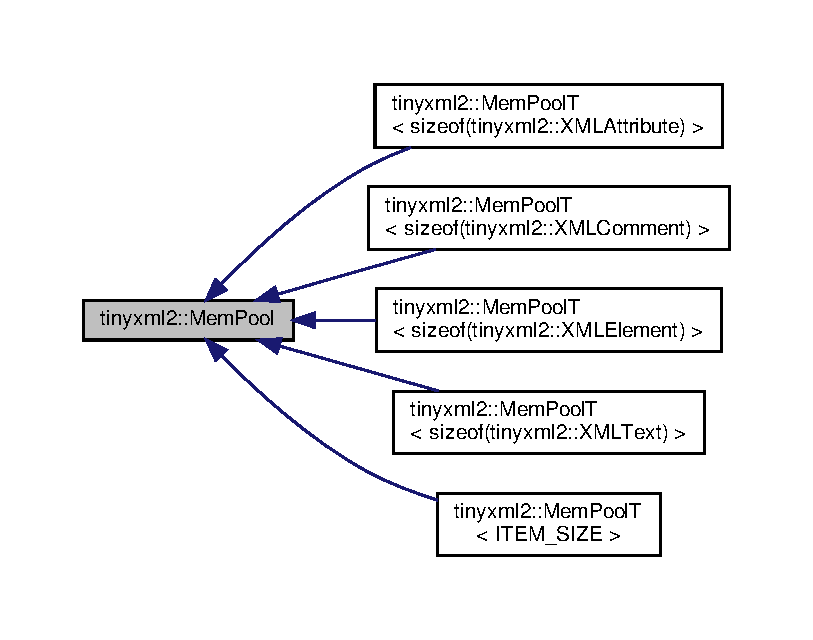
\includegraphics[width=350pt]{classtinyxml2_1_1_mem_pool__inherit__graph}
\end{center}
\end{figure}
\subsection*{Public Member Functions}
\begin{DoxyCompactItemize}
\item 
\mbox{\Hypertarget{classtinyxml2_1_1_mem_pool_a0c518d49e3a94bde566f61e13b7240bb}\label{classtinyxml2_1_1_mem_pool_a0c518d49e3a94bde566f61e13b7240bb}} 
virtual int {\bfseries Item\+Size} () const =0
\item 
\mbox{\Hypertarget{classtinyxml2_1_1_mem_pool_a4f977b5fed752c0bbfe5295f469d6449}\label{classtinyxml2_1_1_mem_pool_a4f977b5fed752c0bbfe5295f469d6449}} 
virtual void $\ast$ {\bfseries Alloc} ()=0
\item 
\mbox{\Hypertarget{classtinyxml2_1_1_mem_pool_a49e3bfac2cba2ebd6776b31e571f64f7}\label{classtinyxml2_1_1_mem_pool_a49e3bfac2cba2ebd6776b31e571f64f7}} 
virtual void {\bfseries Free} (void $\ast$)=0
\item 
\mbox{\Hypertarget{classtinyxml2_1_1_mem_pool_ac5804dd1387b2e4de5eef710076a0db1}\label{classtinyxml2_1_1_mem_pool_ac5804dd1387b2e4de5eef710076a0db1}} 
virtual void {\bfseries Set\+Tracked} ()=0
\end{DoxyCompactItemize}


The documentation for this class was generated from the following file\+:\begin{DoxyCompactItemize}
\item 
/home/ijlee/workspace/sdmt/src/tinyxml2.\+h\end{DoxyCompactItemize}

\hypertarget{classtinyxml2_1_1_mem_pool_t}{}\section{tinyxml2\+:\+:Mem\+PoolT$<$ I\+T\+E\+M\+\_\+\+S\+I\+ZE $>$ Class Template Reference}
\label{classtinyxml2_1_1_mem_pool_t}\index{tinyxml2\+::\+Mem\+Pool\+T$<$ I\+T\+E\+M\+\_\+\+S\+I\+Z\+E $>$@{tinyxml2\+::\+Mem\+Pool\+T$<$ I\+T\+E\+M\+\_\+\+S\+I\+Z\+E $>$}}


Inheritance diagram for tinyxml2\+:\+:Mem\+PoolT$<$ I\+T\+E\+M\+\_\+\+S\+I\+ZE $>$\+:
\nopagebreak
\begin{figure}[H]
\begin{center}
\leavevmode
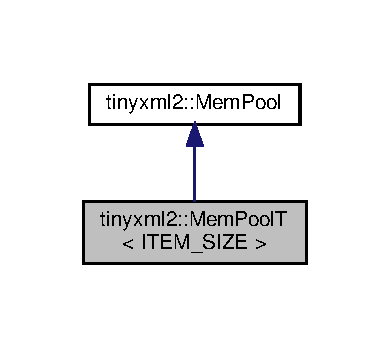
\includegraphics[width=187pt]{classtinyxml2_1_1_mem_pool_t__inherit__graph}
\end{center}
\end{figure}


Collaboration diagram for tinyxml2\+:\+:Mem\+PoolT$<$ I\+T\+E\+M\+\_\+\+S\+I\+ZE $>$\+:
\nopagebreak
\begin{figure}[H]
\begin{center}
\leavevmode
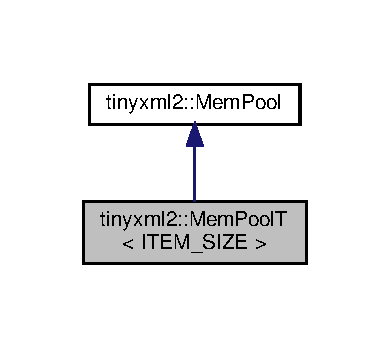
\includegraphics[width=187pt]{classtinyxml2_1_1_mem_pool_t__coll__graph}
\end{center}
\end{figure}
\subsection*{Public Types}
\begin{DoxyCompactItemize}
\item 
\mbox{\Hypertarget{classtinyxml2_1_1_mem_pool_t_a04cf45156e6f913f93972869ff8a1d94}\label{classtinyxml2_1_1_mem_pool_t_a04cf45156e6f913f93972869ff8a1d94}} 
enum \{ {\bfseries I\+T\+E\+M\+S\+\_\+\+P\+E\+R\+\_\+\+B\+L\+O\+CK} = (4 $\ast$ 1024) / I\+T\+E\+M\+\_\+\+S\+I\+ZE
 \}
\end{DoxyCompactItemize}
\subsection*{Public Member Functions}
\begin{DoxyCompactItemize}
\item 
\mbox{\Hypertarget{classtinyxml2_1_1_mem_pool_t_a22d595caa0e9d23aa080f49ca6475fdd}\label{classtinyxml2_1_1_mem_pool_t_a22d595caa0e9d23aa080f49ca6475fdd}} 
void {\bfseries Clear} ()
\item 
\mbox{\Hypertarget{classtinyxml2_1_1_mem_pool_t_a54e4d9b343459ef1731314a99877ff35}\label{classtinyxml2_1_1_mem_pool_t_a54e4d9b343459ef1731314a99877ff35}} 
virtual int {\bfseries Item\+Size} () const
\item 
\mbox{\Hypertarget{classtinyxml2_1_1_mem_pool_t_a445a6c80151ba6268b24ec62a7c84d74}\label{classtinyxml2_1_1_mem_pool_t_a445a6c80151ba6268b24ec62a7c84d74}} 
int {\bfseries Current\+Allocs} () const
\item 
\mbox{\Hypertarget{classtinyxml2_1_1_mem_pool_t_a810fd2b0caf56b8b688e55f2768f96c7}\label{classtinyxml2_1_1_mem_pool_t_a810fd2b0caf56b8b688e55f2768f96c7}} 
virtual void $\ast$ {\bfseries Alloc} ()
\item 
\mbox{\Hypertarget{classtinyxml2_1_1_mem_pool_t_a408ce0918e9d3d5e5e1cc4896944875f}\label{classtinyxml2_1_1_mem_pool_t_a408ce0918e9d3d5e5e1cc4896944875f}} 
virtual void {\bfseries Free} (void $\ast$mem)
\item 
\mbox{\Hypertarget{classtinyxml2_1_1_mem_pool_t_a47eefbd934ef70d973ea41d41ab5f239}\label{classtinyxml2_1_1_mem_pool_t_a47eefbd934ef70d973ea41d41ab5f239}} 
void {\bfseries Trace} (const char $\ast$name)
\item 
\mbox{\Hypertarget{classtinyxml2_1_1_mem_pool_t_aee3c611215ae08cce41a940bf2763027}\label{classtinyxml2_1_1_mem_pool_t_aee3c611215ae08cce41a940bf2763027}} 
void {\bfseries Set\+Tracked} ()
\item 
\mbox{\Hypertarget{classtinyxml2_1_1_mem_pool_t_a3bcdc302ae15d2810e11192321a8f5f1}\label{classtinyxml2_1_1_mem_pool_t_a3bcdc302ae15d2810e11192321a8f5f1}} 
int {\bfseries Untracked} () const
\end{DoxyCompactItemize}


The documentation for this class was generated from the following file\+:\begin{DoxyCompactItemize}
\item 
/home/ijlee/workspace/sdmt/src/tinyxml2.\+h\end{DoxyCompactItemize}

\hypertarget{class_s_d_m_t}{}\section{S\+D\+MT Class Reference}
\label{class_s_d_m_t}\index{S\+D\+MT@{S\+D\+MT}}


a singleton class that provides A\+P\+Is of \hyperlink{class_s_d_m_t}{S\+D\+MT}  




{\ttfamily \#include $<$sdmt.\+h$>$}

\subsection*{Classes}
\begin{DoxyCompactItemize}
\item 
struct \hyperlink{struct_s_d_m_t_1_1_ckpt_info}{Ckpt\+Info}
\begin{DoxyCompactList}\small\item\em checkpoint info \end{DoxyCompactList}\item 
struct \hyperlink{struct_s_d_m_t_1_1_segment}{Segment}
\begin{DoxyCompactList}\small\item\em a chunk of memory which is the unit of allocation and management \end{DoxyCompactList}\end{DoxyCompactItemize}
\subsection*{Public Types}
\begin{DoxyCompactItemize}
\item 
typedef std\+::unordered\+\_\+map$<$ std\+::string, \hyperlink{struct_s_d_m_t_1_1_segment}{Segment} $>$ \hyperlink{class_s_d_m_t_ab60c4624d197b2cf048ca65243d5bc53}{Segment\+Map}\hypertarget{class_s_d_m_t_ab60c4624d197b2cf048ca65243d5bc53}{}\label{class_s_d_m_t_ab60c4624d197b2cf048ca65243d5bc53}

\begin{DoxyCompactList}\small\item\em hash map that mapping name of \hyperlink{struct_s_d_m_t_1_1_segment}{Segment} and \hyperlink{struct_s_d_m_t_1_1_segment}{Segment} \end{DoxyCompactList}\end{DoxyCompactItemize}
\subsection*{Public Member Functions}
\begin{DoxyCompactItemize}
\item 
\hyperlink{class_s_d_m_t_a93fb108be06183e27b33ca23919c0ff9}{S\+D\+MT} ()\hypertarget{class_s_d_m_t_a93fb108be06183e27b33ca23919c0ff9}{}\label{class_s_d_m_t_a93fb108be06183e27b33ca23919c0ff9}

\begin{DoxyCompactList}\small\item\em \hyperlink{class_s_d_m_t}{S\+D\+MT} constructor. \end{DoxyCompactList}\end{DoxyCompactItemize}
\subsection*{Static Public Member Functions}
\begin{DoxyCompactItemize}
\item 
static \hyperlink{class_s_d_m_t}{S\+D\+MT} \& \hyperlink{class_s_d_m_t_a58f43a16728b4d990ca10c1efe70740f}{get\+\_\+manager} ()
\begin{DoxyCompactList}\small\item\em \mbox{[}static\mbox{]}get \hyperlink{class_s_d_m_t}{S\+D\+MT} manager singleton \end{DoxyCompactList}\item 
static S\+D\+M\+T\+\_\+\+Code \hyperlink{class_s_d_m_t_a6d177e96e25e852acc3f9bd273215f3c}{init} (std\+::string config)
\begin{DoxyCompactList}\small\item\em \mbox{[}static\mbox{]}init sdmt(simulation process and data management) \end{DoxyCompactList}\item 
static S\+D\+M\+T\+\_\+\+Code \hyperlink{class_s_d_m_t_a0ee438570acc7a74676693b86fdc94a9}{start} ()
\begin{DoxyCompactList}\small\item\em \mbox{[}static\mbox{]}start sdmt(simulation process and data management) \end{DoxyCompactList}\item 
static S\+D\+M\+T\+\_\+\+Code \hyperlink{class_s_d_m_t_af56c324524d2b8684f268b78d7e64534}{finalize} ()
\begin{DoxyCompactList}\small\item\em \mbox{[}static\mbox{]}finalize sdmt(simulation process and data management) \end{DoxyCompactList}\item 
static S\+D\+M\+T\+\_\+\+Code \hyperlink{class_s_d_m_t_a4da48bca02cad8bfe78a1bafec4a1b1f}{register\+\_\+segment} (std\+::string name, S\+D\+M\+T\+\_\+\+VT vt, S\+D\+M\+T\+\_\+\+DT dt, std\+::vector$<$ int $>$ dim)
\begin{DoxyCompactList}\small\item\em \mbox{[}static\mbox{]}register a \hyperlink{struct_s_d_m_t_1_1_segment}{Segment} to sdmt manager \end{DoxyCompactList}\item 
static S\+D\+M\+T\+\_\+\+Code \hyperlink{class_s_d_m_t_a65fbeacab1acd95ab0197af42de6b3b0}{checkpoint} ()
\begin{DoxyCompactList}\small\item\em \mbox{[}static\mbox{]}create a checkpoint of a \hyperlink{struct_s_d_m_t_1_1_segment}{Segment} \end{DoxyCompactList}\item 
static S\+D\+M\+T\+\_\+\+Code \hyperlink{class_s_d_m_t_a3a3723f019f53a371c2c3b49efbed0f5}{recover} ()
\begin{DoxyCompactList}\small\item\em \mbox{[}static\mbox{]}recover checkpointed Segments \end{DoxyCompactList}\item 
static \hyperlink{struct_s_d_m_t_1_1_segment}{Segment} \hyperlink{class_s_d_m_t_a8dfbf78068663cc21ff1e7f15fca6e55}{get\+\_\+segment} (std\+::string name)
\begin{DoxyCompactList}\small\item\em \mbox{[}static\mbox{]} get \hyperlink{struct_s_d_m_t_1_1_segment}{Segment} \end{DoxyCompactList}\item 
static int $\ast$ \hyperlink{class_s_d_m_t_a31a70a690a9215643afaf9ef1abb35f1}{intptr} (std\+::string name)
\begin{DoxyCompactList}\small\item\em \mbox{[}static\mbox{]}get memory pointer of registered \hyperlink{struct_s_d_m_t_1_1_segment}{Segment} \end{DoxyCompactList}\item 
static long $\ast$ \hyperlink{class_s_d_m_t_ac36749f096dc877e0ff4bbd7370eebe6}{longptr} (std\+::string name)
\begin{DoxyCompactList}\small\item\em \mbox{[}static\mbox{]}get memory pointer of registered \hyperlink{struct_s_d_m_t_1_1_segment}{Segment} \end{DoxyCompactList}\item 
static float $\ast$ \hyperlink{class_s_d_m_t_a44a9454c55626de3cf5e9b37b9016d6c}{floatptr} (std\+::string name)
\begin{DoxyCompactList}\small\item\em \mbox{[}static\mbox{]}get memory pointer of registered \hyperlink{struct_s_d_m_t_1_1_segment}{Segment} \end{DoxyCompactList}\item 
static double $\ast$ \hyperlink{class_s_d_m_t_ab51288f0cabdd3a1ff1db6920c1096f7}{doubleptr} (std\+::string name)
\begin{DoxyCompactList}\small\item\em \mbox{[}static\mbox{]}get memory pointer of registered \hyperlink{struct_s_d_m_t_1_1_segment}{Segment} \end{DoxyCompactList}\end{DoxyCompactItemize}


\subsection{Detailed Description}
a singleton class that provides A\+P\+Is of \hyperlink{class_s_d_m_t}{S\+D\+MT} 

\begin{DoxyItemize}
\item assign a data chunk to be managed in simulation process\end{DoxyItemize}
\begin{DoxyItemize}
\item make snapshot checkpoint during iterative simulation and recovery intermediate results for restart\end{DoxyItemize}
\begin{DoxyItemize}
\item collect statistics about data reference\end{DoxyItemize}
\begin{DoxyAuthor}{Author}
Ilju Lee, \href{mailto:ijlee@kdb.snu.ac.kr}{\tt ijlee@kdb.\+snu.\+ac.\+kr} 

Jinyon Kim, \href{mailto:jykim@kdb.snu.ac.kr}{\tt jykim@kdb.\+snu.\+ac.\+kr} 

Hyerim Jeon, \href{mailto:hrjeon@kdb.snu.ac.kr}{\tt hrjeon@kdb.\+snu.\+ac.\+kr} 
\end{DoxyAuthor}


\subsection{Member Function Documentation}
\index{S\+D\+MT@{S\+D\+MT}!checkpoint@{checkpoint}}
\index{checkpoint@{checkpoint}!S\+D\+MT@{S\+D\+MT}}
\subsubsection[{\texorpdfstring{checkpoint()}{checkpoint()}}]{\setlength{\rightskip}{0pt plus 5cm}static S\+D\+M\+T\+\_\+\+Code S\+D\+M\+T\+::checkpoint (
\begin{DoxyParamCaption}
{}
\end{DoxyParamCaption}
)\hspace{0.3cm}{\ttfamily [inline]}, {\ttfamily [static]}}\hypertarget{class_s_d_m_t_a65fbeacab1acd95ab0197af42de6b3b0}{}\label{class_s_d_m_t_a65fbeacab1acd95ab0197af42de6b3b0}


\mbox{[}static\mbox{]}create a checkpoint of a \hyperlink{struct_s_d_m_t_1_1_segment}{Segment} 

\begin{DoxyReturn}{Returns}
status code 
\end{DoxyReturn}
\index{S\+D\+MT@{S\+D\+MT}!doubleptr@{doubleptr}}
\index{doubleptr@{doubleptr}!S\+D\+MT@{S\+D\+MT}}
\subsubsection[{\texorpdfstring{doubleptr(std\+::string name)}{doubleptr(std::string name)}}]{\setlength{\rightskip}{0pt plus 5cm}static double$\ast$ S\+D\+M\+T\+::doubleptr (
\begin{DoxyParamCaption}
\item[{std\+::string}]{name}
\end{DoxyParamCaption}
)\hspace{0.3cm}{\ttfamily [inline]}, {\ttfamily [static]}}\hypertarget{class_s_d_m_t_ab51288f0cabdd3a1ff1db6920c1096f7}{}\label{class_s_d_m_t_ab51288f0cabdd3a1ff1db6920c1096f7}


\mbox{[}static\mbox{]}get memory pointer of registered \hyperlink{struct_s_d_m_t_1_1_segment}{Segment} 


\begin{DoxyParams}{Parameters}
{\em name} & name of the \hyperlink{struct_s_d_m_t_1_1_segment}{Segment} \\
\hline
\end{DoxyParams}
\begin{DoxyReturn}{Returns}
double pointer, null if name is incorrect 
\end{DoxyReturn}
\index{S\+D\+MT@{S\+D\+MT}!finalize@{finalize}}
\index{finalize@{finalize}!S\+D\+MT@{S\+D\+MT}}
\subsubsection[{\texorpdfstring{finalize()}{finalize()}}]{\setlength{\rightskip}{0pt plus 5cm}static S\+D\+M\+T\+\_\+\+Code S\+D\+M\+T\+::finalize (
\begin{DoxyParamCaption}
{}
\end{DoxyParamCaption}
)\hspace{0.3cm}{\ttfamily [inline]}, {\ttfamily [static]}}\hypertarget{class_s_d_m_t_af56c324524d2b8684f268b78d7e64534}{}\label{class_s_d_m_t_af56c324524d2b8684f268b78d7e64534}


\mbox{[}static\mbox{]}finalize sdmt(simulation process and data management) 

\begin{DoxyReturn}{Returns}
status code 
\end{DoxyReturn}
\index{S\+D\+MT@{S\+D\+MT}!floatptr@{floatptr}}
\index{floatptr@{floatptr}!S\+D\+MT@{S\+D\+MT}}
\subsubsection[{\texorpdfstring{floatptr(std\+::string name)}{floatptr(std::string name)}}]{\setlength{\rightskip}{0pt plus 5cm}static float$\ast$ S\+D\+M\+T\+::floatptr (
\begin{DoxyParamCaption}
\item[{std\+::string}]{name}
\end{DoxyParamCaption}
)\hspace{0.3cm}{\ttfamily [inline]}, {\ttfamily [static]}}\hypertarget{class_s_d_m_t_a44a9454c55626de3cf5e9b37b9016d6c}{}\label{class_s_d_m_t_a44a9454c55626de3cf5e9b37b9016d6c}


\mbox{[}static\mbox{]}get memory pointer of registered \hyperlink{struct_s_d_m_t_1_1_segment}{Segment} 


\begin{DoxyParams}{Parameters}
{\em name} & name of the \hyperlink{struct_s_d_m_t_1_1_segment}{Segment} \\
\hline
\end{DoxyParams}
\begin{DoxyReturn}{Returns}
float pointer, null if name is incorrect 
\end{DoxyReturn}
\index{S\+D\+MT@{S\+D\+MT}!get\+\_\+manager@{get\+\_\+manager}}
\index{get\+\_\+manager@{get\+\_\+manager}!S\+D\+MT@{S\+D\+MT}}
\subsubsection[{\texorpdfstring{get\+\_\+manager()}{get_manager()}}]{\setlength{\rightskip}{0pt plus 5cm}static {\bf S\+D\+MT}\& S\+D\+M\+T\+::get\+\_\+manager (
\begin{DoxyParamCaption}
{}
\end{DoxyParamCaption}
)\hspace{0.3cm}{\ttfamily [inline]}, {\ttfamily [static]}}\hypertarget{class_s_d_m_t_a58f43a16728b4d990ca10c1efe70740f}{}\label{class_s_d_m_t_a58f43a16728b4d990ca10c1efe70740f}


\mbox{[}static\mbox{]}get \hyperlink{class_s_d_m_t}{S\+D\+MT} manager singleton 

\begin{DoxyReturn}{Returns}
static \hyperlink{class_s_d_m_t}{S\+D\+MT} manager 
\end{DoxyReturn}
\index{S\+D\+MT@{S\+D\+MT}!get\+\_\+segment@{get\+\_\+segment}}
\index{get\+\_\+segment@{get\+\_\+segment}!S\+D\+MT@{S\+D\+MT}}
\subsubsection[{\texorpdfstring{get\+\_\+segment(std\+::string name)}{get_segment(std::string name)}}]{\setlength{\rightskip}{0pt plus 5cm}static {\bf Segment} S\+D\+M\+T\+::get\+\_\+segment (
\begin{DoxyParamCaption}
\item[{std\+::string}]{name}
\end{DoxyParamCaption}
)\hspace{0.3cm}{\ttfamily [inline]}, {\ttfamily [static]}}\hypertarget{class_s_d_m_t_a8dfbf78068663cc21ff1e7f15fca6e55}{}\label{class_s_d_m_t_a8dfbf78068663cc21ff1e7f15fca6e55}


\mbox{[}static\mbox{]} get \hyperlink{struct_s_d_m_t_1_1_segment}{Segment} 

\begin{DoxyReturn}{Returns}
\hyperlink{struct_s_d_m_t_1_1_segment}{Segment}, null if name is incorrect 
\end{DoxyReturn}
\index{S\+D\+MT@{S\+D\+MT}!init@{init}}
\index{init@{init}!S\+D\+MT@{S\+D\+MT}}
\subsubsection[{\texorpdfstring{init(std\+::string config)}{init(std::string config)}}]{\setlength{\rightskip}{0pt plus 5cm}static S\+D\+M\+T\+\_\+\+Code S\+D\+M\+T\+::init (
\begin{DoxyParamCaption}
\item[{std\+::string}]{config}
\end{DoxyParamCaption}
)\hspace{0.3cm}{\ttfamily [inline]}, {\ttfamily [static]}}\hypertarget{class_s_d_m_t_a6d177e96e25e852acc3f9bd273215f3c}{}\label{class_s_d_m_t_a6d177e96e25e852acc3f9bd273215f3c}


\mbox{[}static\mbox{]}init sdmt(simulation process and data management) 


\begin{DoxyParams}{Parameters}
{\em config} & path of config file \\
\hline
\end{DoxyParams}
\begin{DoxyReturn}{Returns}
status code 
\end{DoxyReturn}
\index{S\+D\+MT@{S\+D\+MT}!intptr@{intptr}}
\index{intptr@{intptr}!S\+D\+MT@{S\+D\+MT}}
\subsubsection[{\texorpdfstring{intptr(std\+::string name)}{intptr(std::string name)}}]{\setlength{\rightskip}{0pt plus 5cm}static int$\ast$ S\+D\+M\+T\+::intptr (
\begin{DoxyParamCaption}
\item[{std\+::string}]{name}
\end{DoxyParamCaption}
)\hspace{0.3cm}{\ttfamily [inline]}, {\ttfamily [static]}}\hypertarget{class_s_d_m_t_a31a70a690a9215643afaf9ef1abb35f1}{}\label{class_s_d_m_t_a31a70a690a9215643afaf9ef1abb35f1}


\mbox{[}static\mbox{]}get memory pointer of registered \hyperlink{struct_s_d_m_t_1_1_segment}{Segment} 


\begin{DoxyParams}{Parameters}
{\em name} & name of the \hyperlink{struct_s_d_m_t_1_1_segment}{Segment} \\
\hline
\end{DoxyParams}
\begin{DoxyReturn}{Returns}
integer pointer, null if name is incorrect 
\end{DoxyReturn}
\index{S\+D\+MT@{S\+D\+MT}!longptr@{longptr}}
\index{longptr@{longptr}!S\+D\+MT@{S\+D\+MT}}
\subsubsection[{\texorpdfstring{longptr(std\+::string name)}{longptr(std::string name)}}]{\setlength{\rightskip}{0pt plus 5cm}static long$\ast$ S\+D\+M\+T\+::longptr (
\begin{DoxyParamCaption}
\item[{std\+::string}]{name}
\end{DoxyParamCaption}
)\hspace{0.3cm}{\ttfamily [inline]}, {\ttfamily [static]}}\hypertarget{class_s_d_m_t_ac36749f096dc877e0ff4bbd7370eebe6}{}\label{class_s_d_m_t_ac36749f096dc877e0ff4bbd7370eebe6}


\mbox{[}static\mbox{]}get memory pointer of registered \hyperlink{struct_s_d_m_t_1_1_segment}{Segment} 


\begin{DoxyParams}{Parameters}
{\em name} & name of the \hyperlink{struct_s_d_m_t_1_1_segment}{Segment} \\
\hline
\end{DoxyParams}
\begin{DoxyReturn}{Returns}
long integer pointer, null if name is incorrect 
\end{DoxyReturn}
\index{S\+D\+MT@{S\+D\+MT}!recover@{recover}}
\index{recover@{recover}!S\+D\+MT@{S\+D\+MT}}
\subsubsection[{\texorpdfstring{recover()}{recover()}}]{\setlength{\rightskip}{0pt plus 5cm}static S\+D\+M\+T\+\_\+\+Code S\+D\+M\+T\+::recover (
\begin{DoxyParamCaption}
{}
\end{DoxyParamCaption}
)\hspace{0.3cm}{\ttfamily [inline]}, {\ttfamily [static]}}\hypertarget{class_s_d_m_t_a3a3723f019f53a371c2c3b49efbed0f5}{}\label{class_s_d_m_t_a3a3723f019f53a371c2c3b49efbed0f5}


\mbox{[}static\mbox{]}recover checkpointed Segments 

\begin{DoxyReturn}{Returns}
status code 
\end{DoxyReturn}
\index{S\+D\+MT@{S\+D\+MT}!register\+\_\+segment@{register\+\_\+segment}}
\index{register\+\_\+segment@{register\+\_\+segment}!S\+D\+MT@{S\+D\+MT}}
\subsubsection[{\texorpdfstring{register\+\_\+segment(std\+::string name, S\+D\+M\+T\+\_\+\+V\+T vt, S\+D\+M\+T\+\_\+\+D\+T dt, std\+::vector$<$ int $>$ dim)}{register_segment(std::string name, SDMT_VT vt, SDMT_DT dt, std::vector< int > dim)}}]{\setlength{\rightskip}{0pt plus 5cm}static S\+D\+M\+T\+\_\+\+Code S\+D\+M\+T\+::register\+\_\+segment (
\begin{DoxyParamCaption}
\item[{std\+::string}]{name, }
\item[{S\+D\+M\+T\+\_\+\+VT}]{vt, }
\item[{S\+D\+M\+T\+\_\+\+DT}]{dt, }
\item[{std\+::vector$<$ int $>$}]{dim}
\end{DoxyParamCaption}
)\hspace{0.3cm}{\ttfamily [inline]}, {\ttfamily [static]}}\hypertarget{class_s_d_m_t_a4da48bca02cad8bfe78a1bafec4a1b1f}{}\label{class_s_d_m_t_a4da48bca02cad8bfe78a1bafec4a1b1f}


\mbox{[}static\mbox{]}register a \hyperlink{struct_s_d_m_t_1_1_segment}{Segment} to sdmt manager 


\begin{DoxyParams}{Parameters}
{\em name} & name of the \hyperlink{struct_s_d_m_t_1_1_segment}{Segment} \\
\hline
{\em vt} & value type \\
\hline
{\em dt} & data type \\
\hline
{\em dim} & size of each dimension \\
\hline
\end{DoxyParams}
\begin{DoxyReturn}{Returns}
status code 
\end{DoxyReturn}
\index{S\+D\+MT@{S\+D\+MT}!start@{start}}
\index{start@{start}!S\+D\+MT@{S\+D\+MT}}
\subsubsection[{\texorpdfstring{start()}{start()}}]{\setlength{\rightskip}{0pt plus 5cm}static S\+D\+M\+T\+\_\+\+Code S\+D\+M\+T\+::start (
\begin{DoxyParamCaption}
{}
\end{DoxyParamCaption}
)\hspace{0.3cm}{\ttfamily [inline]}, {\ttfamily [static]}}\hypertarget{class_s_d_m_t_a0ee438570acc7a74676693b86fdc94a9}{}\label{class_s_d_m_t_a0ee438570acc7a74676693b86fdc94a9}


\mbox{[}static\mbox{]}start sdmt(simulation process and data management) 

\begin{DoxyReturn}{Returns}
status code 
\end{DoxyReturn}


The documentation for this class was generated from the following files\+:\begin{DoxyCompactItemize}
\item 
/raid/users/ijlee/workspace/hpc/src/sdmt.\+h\item 
/raid/users/ijlee/workspace/hpc/src/sdmt.\+cc\end{DoxyCompactItemize}

\hypertarget{struct_s_d_m_t_1_1_segment}{}\section{S\+D\+MT\+:\+:Segment Struct Reference}
\label{struct_s_d_m_t_1_1_segment}\index{S\+D\+M\+T\+::\+Segment@{S\+D\+M\+T\+::\+Segment}}


a chunk of memory which is the unit of allocation and management  




{\ttfamily \#include $<$sdmt.\+h$>$}

\subsection*{Public Member Functions}
\begin{DoxyCompactItemize}
\item 
\hyperlink{struct_s_d_m_t_1_1_segment_a0f4b0aa7fa5596a96a84129f010f19b6}{Segment} ()\hypertarget{struct_s_d_m_t_1_1_segment_a0f4b0aa7fa5596a96a84129f010f19b6}{}\label{struct_s_d_m_t_1_1_segment_a0f4b0aa7fa5596a96a84129f010f19b6}

\begin{DoxyCompactList}\small\item\em create a null \hyperlink{struct_s_d_m_t_1_1_segment}{Segment} \end{DoxyCompactList}\item 
\hyperlink{struct_s_d_m_t_1_1_segment_a386954456945a0bfb2634e6e3ae2b6a6}{Segment} (int32\+\_\+t id, S\+D\+M\+T\+\_\+\+VT vt, S\+D\+M\+T\+\_\+\+DT dt, std\+::vector$<$ int $>$ dim, int32\+\_\+t esize, void $\ast$ptr)
\begin{DoxyCompactList}\small\item\em \hyperlink{struct_s_d_m_t_1_1_segment}{S\+D\+M\+T\+::\+Segment} constructor. \end{DoxyCompactList}\item 
\hyperlink{struct_s_d_m_t_1_1_segment_a119578504b0ab9d498d506aea0a169f5}{Segment} (const \hyperlink{struct_s_d_m_t_1_1_segment}{Segment} \&other)
\begin{DoxyCompactList}\small\item\em \hyperlink{struct_s_d_m_t_1_1_segment}{S\+D\+M\+T\+::\+Segment} copy constructor. \end{DoxyCompactList}\item 
\hyperlink{struct_s_d_m_t_1_1_segment_a9da129d3aacb44861d18c2e97986aa55}{$\sim$\+Segment} ()\hypertarget{struct_s_d_m_t_1_1_segment_a9da129d3aacb44861d18c2e97986aa55}{}\label{struct_s_d_m_t_1_1_segment_a9da129d3aacb44861d18c2e97986aa55}

\begin{DoxyCompactList}\small\item\em \hyperlink{struct_s_d_m_t_1_1_segment}{S\+D\+M\+T\+::\+Segment} destructor. \end{DoxyCompactList}\end{DoxyCompactItemize}
\subsection*{Public Attributes}
\begin{DoxyCompactItemize}
\item 
int32\+\_\+t \hyperlink{struct_s_d_m_t_1_1_segment_af2364bde7b35f4cd691763d3e62b97f2}{m\+\_\+id}\hypertarget{struct_s_d_m_t_1_1_segment_af2364bde7b35f4cd691763d3e62b97f2}{}\label{struct_s_d_m_t_1_1_segment_af2364bde7b35f4cd691763d3e62b97f2}

\begin{DoxyCompactList}\small\item\em id of \hyperlink{struct_s_d_m_t_1_1_segment}{Segment} \end{DoxyCompactList}\item 
S\+D\+M\+T\+\_\+\+VT \hyperlink{struct_s_d_m_t_1_1_segment_a35496150825a45541dd29919a4351e32}{m\+\_\+valuetype}\hypertarget{struct_s_d_m_t_1_1_segment_a35496150825a45541dd29919a4351e32}{}\label{struct_s_d_m_t_1_1_segment_a35496150825a45541dd29919a4351e32}

\begin{DoxyCompactList}\small\item\em value type of elements in \hyperlink{struct_s_d_m_t_1_1_segment}{Segment} \end{DoxyCompactList}\item 
S\+D\+M\+T\+\_\+\+DT \hyperlink{struct_s_d_m_t_1_1_segment_a567eec58da0032cbcd0cb9b83c2e8dbd}{m\+\_\+datatype}\hypertarget{struct_s_d_m_t_1_1_segment_a567eec58da0032cbcd0cb9b83c2e8dbd}{}\label{struct_s_d_m_t_1_1_segment_a567eec58da0032cbcd0cb9b83c2e8dbd}

\begin{DoxyCompactList}\small\item\em type of data structure \end{DoxyCompactList}\item 
std\+::vector$<$ int $>$ \hyperlink{struct_s_d_m_t_1_1_segment_af472ea128d3ef6acb84a2e4306179a1a}{m\+\_\+dimension}\hypertarget{struct_s_d_m_t_1_1_segment_af472ea128d3ef6acb84a2e4306179a1a}{}\label{struct_s_d_m_t_1_1_segment_af472ea128d3ef6acb84a2e4306179a1a}

\begin{DoxyCompactList}\small\item\em dimension of data \end{DoxyCompactList}\item 
std\+::vector$<$ int $>$ \hyperlink{struct_s_d_m_t_1_1_segment_a9ba0ecef2a5986705e0336c824dc61a9}{m\+\_\+strides}\hypertarget{struct_s_d_m_t_1_1_segment_a9ba0ecef2a5986705e0336c824dc61a9}{}\label{struct_s_d_m_t_1_1_segment_a9ba0ecef2a5986705e0336c824dc61a9}

\begin{DoxyCompactList}\small\item\em byte strides for each index \end{DoxyCompactList}\item 
int32\+\_\+t \hyperlink{struct_s_d_m_t_1_1_segment_abf1844991a9c39778c83fb90bdc95da7}{m\+\_\+esize}\hypertarget{struct_s_d_m_t_1_1_segment_abf1844991a9c39778c83fb90bdc95da7}{}\label{struct_s_d_m_t_1_1_segment_abf1844991a9c39778c83fb90bdc95da7}

\begin{DoxyCompactList}\small\item\em byte size of an element in \hyperlink{struct_s_d_m_t_1_1_segment}{Segment} \end{DoxyCompactList}\item 
void $\ast$ \hyperlink{struct_s_d_m_t_1_1_segment_ad07915cd3d0e07df6338cec28ad077d8}{m\+\_\+ptr}\hypertarget{struct_s_d_m_t_1_1_segment_ad07915cd3d0e07df6338cec28ad077d8}{}\label{struct_s_d_m_t_1_1_segment_ad07915cd3d0e07df6338cec28ad077d8}

\begin{DoxyCompactList}\small\item\em memory pointer of data \end{DoxyCompactList}\end{DoxyCompactItemize}


\subsection{Detailed Description}
a chunk of memory which is the unit of allocation and management 

\subsection{Constructor \& Destructor Documentation}
\index{S\+D\+M\+T\+::\+Segment@{S\+D\+M\+T\+::\+Segment}!Segment@{Segment}}
\index{Segment@{Segment}!S\+D\+M\+T\+::\+Segment@{S\+D\+M\+T\+::\+Segment}}
\subsubsection[{\texorpdfstring{Segment(int32\+\_\+t id, S\+D\+M\+T\+\_\+\+V\+T vt, S\+D\+M\+T\+\_\+\+D\+T dt, std\+::vector$<$ int $>$ dim, int32\+\_\+t esize, void $\ast$ptr)}{Segment(int32_t id, SDMT_VT vt, SDMT_DT dt, std::vector< int > dim, int32_t esize, void *ptr)}}]{\setlength{\rightskip}{0pt plus 5cm}S\+D\+M\+T\+::\+Segment\+::\+Segment (
\begin{DoxyParamCaption}
\item[{int32\+\_\+t}]{id, }
\item[{S\+D\+M\+T\+\_\+\+VT}]{vt, }
\item[{S\+D\+M\+T\+\_\+\+DT}]{dt, }
\item[{std\+::vector$<$ int $>$}]{dim, }
\item[{int32\+\_\+t}]{esize, }
\item[{void $\ast$}]{ptr}
\end{DoxyParamCaption}
)\hspace{0.3cm}{\ttfamily [inline]}}\hypertarget{struct_s_d_m_t_1_1_segment_a386954456945a0bfb2634e6e3ae2b6a6}{}\label{struct_s_d_m_t_1_1_segment_a386954456945a0bfb2634e6e3ae2b6a6}


\hyperlink{struct_s_d_m_t_1_1_segment}{S\+D\+M\+T\+::\+Segment} constructor. 


\begin{DoxyParams}{Parameters}
{\em id} & id of \hyperlink{struct_s_d_m_t_1_1_segment}{Segment} \\
\hline
{\em vt} & value type \\
\hline
{\em dt} & data type \\
\hline
{\em dim} & size of each dimension \\
\hline
{\em esize} & size of an element \\
\hline
{\em ptr} & assigned memory \\
\hline
\end{DoxyParams}
\index{S\+D\+M\+T\+::\+Segment@{S\+D\+M\+T\+::\+Segment}!Segment@{Segment}}
\index{Segment@{Segment}!S\+D\+M\+T\+::\+Segment@{S\+D\+M\+T\+::\+Segment}}
\subsubsection[{\texorpdfstring{Segment(const Segment \&other)}{Segment(const Segment &other)}}]{\setlength{\rightskip}{0pt plus 5cm}S\+D\+M\+T\+::\+Segment\+::\+Segment (
\begin{DoxyParamCaption}
\item[{const {\bf Segment} \&}]{other}
\end{DoxyParamCaption}
)\hspace{0.3cm}{\ttfamily [inline]}}\hypertarget{struct_s_d_m_t_1_1_segment_a119578504b0ab9d498d506aea0a169f5}{}\label{struct_s_d_m_t_1_1_segment_a119578504b0ab9d498d506aea0a169f5}


\hyperlink{struct_s_d_m_t_1_1_segment}{S\+D\+M\+T\+::\+Segment} copy constructor. 


\begin{DoxyParams}{Parameters}
{\em other} & \hyperlink{struct_s_d_m_t_1_1_segment}{Segment} to copy \\
\hline
\end{DoxyParams}


The documentation for this struct was generated from the following file\+:\begin{DoxyCompactItemize}
\item 
/raid/users/ijlee/workspace/hpc/src/sdmt.\+h\end{DoxyCompactItemize}

\hypertarget{classserialize}{}\section{serialize Class Reference}
\label{classserialize}\index{serialize@{serialize}}
\subsection*{Classes}
\begin{DoxyCompactItemize}
\item 
class \hyperlink{classserialize_1_1_i}{I}
\end{DoxyCompactItemize}
\subsection*{Static Public Member Functions}
\begin{DoxyCompactItemize}
\item 
\mbox{\Hypertarget{classserialize_a160d44cc2c19098e5d41224867559ac4}\label{classserialize_a160d44cc2c19098e5d41224867559ac4}} 
static bool {\bfseries LE} ()
\item 
\mbox{\Hypertarget{classserialize_a8b8d6453d506383842486049839f193e}\label{classserialize_a8b8d6453d506383842486049839f193e}} 
static bool {\bfseries Read\+Endian} (istream \&istream\+\_\+)
\item 
\mbox{\Hypertarget{classserialize_ab321f5937ee9bcdf95b2703a461729a5}\label{classserialize_ab321f5937ee9bcdf95b2703a461729a5}} 
static void {\bfseries Write\+Endian} (ostream \&ostream\+\_\+)
\item 
\mbox{\Hypertarget{classserialize_a5e32a337b86a0d42bc249f5341edafca}\label{classserialize_a5e32a337b86a0d42bc249f5341edafca}} 
static istream \& {\bfseries read\+\_\+internal} (istream \&istream\+\_\+, char $\ast$p, uint32\+\_\+t size)
\item 
\mbox{\Hypertarget{classserialize_a0429510b5f6566b1a8d66762436821a2}\label{classserialize_a0429510b5f6566b1a8d66762436821a2}} 
static ostream \& {\bfseries write\+\_\+internal} (ostream \&ostream\+\_\+, const char $\ast$p, uint32\+\_\+t size)
\item 
\mbox{\Hypertarget{classserialize_a5eadc0bfb3b9b949b5229f5907e50ea5}\label{classserialize_a5eadc0bfb3b9b949b5229f5907e50ea5}} 
static istream \& {\bfseries read} (istream \&istream\+\_\+, \hyperlink{classserialize_1_1_i}{I} $\ast$t\+\_\+)
\item 
\mbox{\Hypertarget{classserialize_a5b6a3f5be8847e9e4a3890f2585cf986}\label{classserialize_a5b6a3f5be8847e9e4a3890f2585cf986}} 
static istream \& {\bfseries read} (istream \&istream\+\_\+, std\+::string \&string\+\_\+)
\item 
\mbox{\Hypertarget{classserialize_ae002b9ab2249de365a6c845942029514}\label{classserialize_ae002b9ab2249de365a6c845942029514}} 
static istream \& {\bfseries read} (istream \&istream\+\_\+, char $\ast$str)
\item 
\mbox{\Hypertarget{classserialize_a91d70f9440a38acd0707d3389a86ddac}\label{classserialize_a91d70f9440a38acd0707d3389a86ddac}} 
static istream \& {\bfseries read} (istream \&istream\+\_\+, vector$<$ bool $>$ \&container)
\item 
\mbox{\Hypertarget{classserialize_adc8829fc5ca697394bd4a7564c9f423d}\label{classserialize_adc8829fc5ca697394bd4a7564c9f423d}} 
static ostream \& {\bfseries write} (ostream \&ostream\+\_\+, \hyperlink{classserialize_1_1_i}{I} $\ast$t\+\_\+)
\item 
\mbox{\Hypertarget{classserialize_a1a5216f4e26943f3706768f3503953ed}\label{classserialize_a1a5216f4e26943f3706768f3503953ed}} 
static ostream \& {\bfseries write} (ostream \&ostream\+\_\+, const std\+::string \&string\+\_\+)
\item 
\mbox{\Hypertarget{classserialize_ac145e93c816fd1828e06341bcdf158f5}\label{classserialize_ac145e93c816fd1828e06341bcdf158f5}} 
static ostream \& {\bfseries write} (ostream \&ostream\+\_\+, std\+::string \&string\+\_\+)
\item 
\mbox{\Hypertarget{classserialize_a0ee7cec24d516020dc3bc312dced3fbe}\label{classserialize_a0ee7cec24d516020dc3bc312dced3fbe}} 
static ostream \& {\bfseries write} (ostream \&ostream\+\_\+, const char $\ast$str)
\item 
\mbox{\Hypertarget{classserialize_a36cdd68fcfac62ff04531c92697ddc15}\label{classserialize_a36cdd68fcfac62ff04531c92697ddc15}} 
static ostream \& {\bfseries write} (ostream \&ostream\+\_\+, vector$<$ bool $>$ \&container)
\item 
\mbox{\Hypertarget{classserialize_a314f203661ac9b44fdde84679a282cd6}\label{classserialize_a314f203661ac9b44fdde84679a282cd6}} 
{\footnotesize template$<$typename T $>$ }\\static void {\bfseries Zero\+Mem} (T \&t)
\item 
\mbox{\Hypertarget{classserialize_a320136a20f918b624dec9d5957662c5d}\label{classserialize_a320136a20f918b624dec9d5957662c5d}} 
{\footnotesize template$<$typename T $>$ }\\static istream \& {\bfseries read} (istream \&istream\+\_\+, T \&t\+\_\+)
\item 
\mbox{\Hypertarget{classserialize_a1fbd07f28ae10549a90ff7e82de7a74c}\label{classserialize_a1fbd07f28ae10549a90ff7e82de7a74c}} 
{\footnotesize template$<$typename T $>$ }\\static ostream \& {\bfseries write} (ostream \&ostream\+\_\+, T \&t\+\_\+)
\item 
\mbox{\Hypertarget{classserialize_a45020fbd693acf144c1b391b945118d5}\label{classserialize_a45020fbd693acf144c1b391b945118d5}} 
{\footnotesize template$<$class T $>$ }\\static ostream \& {\bfseries write} (ostream \&ostream\+\_\+, vector$<$ T $>$ \&container)
\item 
\mbox{\Hypertarget{classserialize_afde35e0b366adf2f5b084c270dc84411}\label{classserialize_afde35e0b366adf2f5b084c270dc84411}} 
{\footnotesize template$<$class T $>$ }\\static istream \& {\bfseries read} (istream \&istream\+\_\+, vector$<$ T $>$ \&container)
\item 
\mbox{\Hypertarget{classserialize_adb3cc636ff02dcf157ed343d5d680297}\label{classserialize_adb3cc636ff02dcf157ed343d5d680297}} 
{\footnotesize template$<$class T $>$ }\\static ostream \& {\bfseries write} (ostream \&ostream\+\_\+, vector$<$ T $\ast$$>$ \&container)
\item 
\mbox{\Hypertarget{classserialize_a11bcb1e62b0fd391ccb028ddbc7d5f1c}\label{classserialize_a11bcb1e62b0fd391ccb028ddbc7d5f1c}} 
{\footnotesize template$<$class T $>$ }\\static istream \& {\bfseries read} (istream \&istream\+\_\+, vector$<$ T $\ast$$>$ \&container)
\item 
\mbox{\Hypertarget{classserialize_ae216738aa56130ca850f9a9ef2ef0f50}\label{classserialize_ae216738aa56130ca850f9a9ef2ef0f50}} 
{\footnotesize template$<$class K , class V $>$ }\\static ostream \& {\bfseries write} (ostream \&ostream\+\_\+, map$<$ K, V $>$ \&container)
\item 
\mbox{\Hypertarget{classserialize_a552182305ba9cc5225366c7efdbcc234}\label{classserialize_a552182305ba9cc5225366c7efdbcc234}} 
{\footnotesize template$<$class K , class V $>$ }\\static istream \& {\bfseries read} (istream \&istream\+\_\+, map$<$ K, V $>$ \&container)
\item 
\mbox{\Hypertarget{classserialize_afa31b4e86afe0002929ad60882f0da05}\label{classserialize_afa31b4e86afe0002929ad60882f0da05}} 
{\footnotesize template$<$class K , class V $>$ }\\static ostream \& {\bfseries write} (ostream \&ostream\+\_\+, map$<$ K, V $\ast$$>$ \&container)
\item 
\mbox{\Hypertarget{classserialize_a5f22cd59cd7b7aec597ec19d882a370f}\label{classserialize_a5f22cd59cd7b7aec597ec19d882a370f}} 
{\footnotesize template$<$class K , class V $>$ }\\static istream \& {\bfseries read} (istream \&istream\+\_\+, map$<$ K, V $\ast$$>$ \&container)
\item 
\mbox{\Hypertarget{classserialize_af8a42854f5c3bf6cd650bababc7373ce}\label{classserialize_af8a42854f5c3bf6cd650bababc7373ce}} 
{\footnotesize template$<$class K , class V $>$ }\\static ostream \& {\bfseries write} (ostream \&ostream\+\_\+, unordered\+\_\+map$<$ K, V $>$ \&container)
\item 
\mbox{\Hypertarget{classserialize_a45c50a563b95f2eb500c77f1d35fdbbd}\label{classserialize_a45c50a563b95f2eb500c77f1d35fdbbd}} 
{\footnotesize template$<$class K , class V $>$ }\\static istream \& {\bfseries read} (istream \&istream\+\_\+, unordered\+\_\+map$<$ K, V $>$ \&container)
\item 
\mbox{\Hypertarget{classserialize_a1780a15309c9fd5c1b99aa86c6e655e2}\label{classserialize_a1780a15309c9fd5c1b99aa86c6e655e2}} 
{\footnotesize template$<$class T $>$ }\\static ostream \& {\bfseries write} (ostream \&ostream\+\_\+, set$<$ T $>$ \&container)
\item 
\mbox{\Hypertarget{classserialize_a7bae550a00495e8f4c0d9462293c79fb}\label{classserialize_a7bae550a00495e8f4c0d9462293c79fb}} 
{\footnotesize template$<$class T $>$ }\\static istream \& {\bfseries read} (istream \&istream\+\_\+, set$<$ T $>$ \&container)
\item 
\mbox{\Hypertarget{classserialize_aa319a12913edb58ebca1110e1ac7e8bb}\label{classserialize_aa319a12913edb58ebca1110e1ac7e8bb}} 
{\footnotesize template$<$class T $>$ }\\static ostream \& {\bfseries write} (ostream \&ostream\+\_\+, set$<$ T $\ast$$>$ \&container)
\item 
\mbox{\Hypertarget{classserialize_a571493399ed66abf6d0995bb515b5a22}\label{classserialize_a571493399ed66abf6d0995bb515b5a22}} 
{\footnotesize template$<$class T $>$ }\\static istream \& {\bfseries read} (istream \&istream\+\_\+, set$<$ T $\ast$$>$ \&container)
\item 
\mbox{\Hypertarget{classserialize_a5b803c97c44afea5120153b909760c14}\label{classserialize_a5b803c97c44afea5120153b909760c14}} 
{\footnotesize template$<$class T $>$ }\\static ostream \& {\bfseries write} (ostream \&ostream\+\_\+, list$<$ T $>$ \&container)
\item 
\mbox{\Hypertarget{classserialize_aa69ad254f8192475195666626e8b6f51}\label{classserialize_aa69ad254f8192475195666626e8b6f51}} 
{\footnotesize template$<$class T $>$ }\\static istream \& {\bfseries read} (istream \&istream\+\_\+, list$<$ T $>$ \&container)
\item 
\mbox{\Hypertarget{classserialize_ae6785408dae3f1e69e4d5811f0ee66a4}\label{classserialize_ae6785408dae3f1e69e4d5811f0ee66a4}} 
{\footnotesize template$<$class T $>$ }\\static ostream \& {\bfseries write} (ostream \&ostream\+\_\+, list$<$ T $\ast$$>$ \&container)
\item 
\mbox{\Hypertarget{classserialize_a06514ab5320d9f070ac8739fabeb5b42}\label{classserialize_a06514ab5320d9f070ac8739fabeb5b42}} 
{\footnotesize template$<$class T $>$ }\\static istream \& {\bfseries read} (istream \&istream\+\_\+, list$<$ T $\ast$$>$ \&container)
\end{DoxyCompactItemize}


The documentation for this class was generated from the following file\+:\begin{DoxyCompactItemize}
\item 
/home/ijlee/workspace/sdmt/src/serialization.\+h\end{DoxyCompactItemize}

\hypertarget{classtinyxml2_1_1_str_pair}{}\section{tinyxml2\+:\+:Str\+Pair Class Reference}
\label{classtinyxml2_1_1_str_pair}\index{tinyxml2\+::\+Str\+Pair@{tinyxml2\+::\+Str\+Pair}}
\subsection*{Public Types}
\begin{DoxyCompactItemize}
\item 
\mbox{\Hypertarget{classtinyxml2_1_1_str_pair_a0301ef962e15dd94574431f1c61266c5}\label{classtinyxml2_1_1_str_pair_a0301ef962e15dd94574431f1c61266c5}} 
enum \{ \newline
{\bfseries N\+E\+E\+D\+S\+\_\+\+E\+N\+T\+I\+T\+Y\+\_\+\+P\+R\+O\+C\+E\+S\+S\+I\+NG} = 0x01, 
{\bfseries N\+E\+E\+D\+S\+\_\+\+N\+E\+W\+L\+I\+N\+E\+\_\+\+N\+O\+R\+M\+A\+L\+I\+Z\+A\+T\+I\+ON} = 0x02, 
{\bfseries N\+E\+E\+D\+S\+\_\+\+W\+H\+I\+T\+E\+S\+P\+A\+C\+E\+\_\+\+C\+O\+L\+L\+A\+P\+S\+I\+NG} = 0x04, 
{\bfseries T\+E\+X\+T\+\_\+\+E\+L\+E\+M\+E\+NT} = N\+E\+E\+D\+S\+\_\+\+E\+N\+T\+I\+T\+Y\+\_\+\+P\+R\+O\+C\+E\+S\+S\+I\+NG $\vert$ N\+E\+E\+D\+S\+\_\+\+N\+E\+W\+L\+I\+N\+E\+\_\+\+N\+O\+R\+M\+A\+L\+I\+Z\+A\+T\+I\+ON, 
\newline
{\bfseries T\+E\+X\+T\+\_\+\+E\+L\+E\+M\+E\+N\+T\+\_\+\+L\+E\+A\+V\+E\+\_\+\+E\+N\+T\+I\+T\+I\+ES} = N\+E\+E\+D\+S\+\_\+\+N\+E\+W\+L\+I\+N\+E\+\_\+\+N\+O\+R\+M\+A\+L\+I\+Z\+A\+T\+I\+ON, 
{\bfseries A\+T\+T\+R\+I\+B\+U\+T\+E\+\_\+\+N\+A\+ME} = 0, 
{\bfseries A\+T\+T\+R\+I\+B\+U\+T\+E\+\_\+\+V\+A\+L\+UE} = N\+E\+E\+D\+S\+\_\+\+E\+N\+T\+I\+T\+Y\+\_\+\+P\+R\+O\+C\+E\+S\+S\+I\+NG $\vert$ N\+E\+E\+D\+S\+\_\+\+N\+E\+W\+L\+I\+N\+E\+\_\+\+N\+O\+R\+M\+A\+L\+I\+Z\+A\+T\+I\+ON, 
{\bfseries A\+T\+T\+R\+I\+B\+U\+T\+E\+\_\+\+V\+A\+L\+U\+E\+\_\+\+L\+E\+A\+V\+E\+\_\+\+E\+N\+T\+I\+T\+I\+ES} = N\+E\+E\+D\+S\+\_\+\+N\+E\+W\+L\+I\+N\+E\+\_\+\+N\+O\+R\+M\+A\+L\+I\+Z\+A\+T\+I\+ON, 
\newline
{\bfseries C\+O\+M\+M\+E\+NT} = N\+E\+E\+D\+S\+\_\+\+N\+E\+W\+L\+I\+N\+E\+\_\+\+N\+O\+R\+M\+A\+L\+I\+Z\+A\+T\+I\+ON
 \}
\end{DoxyCompactItemize}
\subsection*{Public Member Functions}
\begin{DoxyCompactItemize}
\item 
\mbox{\Hypertarget{classtinyxml2_1_1_str_pair_a4f05549373394266a1eecba26813c166}\label{classtinyxml2_1_1_str_pair_a4f05549373394266a1eecba26813c166}} 
void {\bfseries Set} (char $\ast$start, char $\ast$end, int flags)
\item 
\mbox{\Hypertarget{classtinyxml2_1_1_str_pair_ad87e3d11330f5e689ba1e7e54c023b57}\label{classtinyxml2_1_1_str_pair_ad87e3d11330f5e689ba1e7e54c023b57}} 
const char $\ast$ {\bfseries Get\+Str} ()
\item 
\mbox{\Hypertarget{classtinyxml2_1_1_str_pair_aca963a7eaa900bfddbea7312f040b39c}\label{classtinyxml2_1_1_str_pair_aca963a7eaa900bfddbea7312f040b39c}} 
bool {\bfseries Empty} () const
\item 
\mbox{\Hypertarget{classtinyxml2_1_1_str_pair_a2baf6230e18333e02ab65d0897ee3941}\label{classtinyxml2_1_1_str_pair_a2baf6230e18333e02ab65d0897ee3941}} 
void {\bfseries Set\+Interned\+Str} (const char $\ast$str)
\item 
\mbox{\Hypertarget{classtinyxml2_1_1_str_pair_a1f82ec6b5bee35ee7466d8565e43b1de}\label{classtinyxml2_1_1_str_pair_a1f82ec6b5bee35ee7466d8565e43b1de}} 
void {\bfseries Set\+Str} (const char $\ast$str, int flags=0)
\item 
\mbox{\Hypertarget{classtinyxml2_1_1_str_pair_a68e6999b7677fa711287ececb9ba317e}\label{classtinyxml2_1_1_str_pair_a68e6999b7677fa711287ececb9ba317e}} 
char $\ast$ {\bfseries Parse\+Text} (char $\ast$in, const char $\ast$end\+Tag, int str\+Flags, int $\ast$cur\+Line\+Num\+Ptr)
\item 
\mbox{\Hypertarget{classtinyxml2_1_1_str_pair_aa6d8998efceba41d87ec2300c70a6085}\label{classtinyxml2_1_1_str_pair_aa6d8998efceba41d87ec2300c70a6085}} 
char $\ast$ {\bfseries Parse\+Name} (char $\ast$in)
\item 
\mbox{\Hypertarget{classtinyxml2_1_1_str_pair_a35f795b1557fe5fdcbd93d3cc5d6b939}\label{classtinyxml2_1_1_str_pair_a35f795b1557fe5fdcbd93d3cc5d6b939}} 
void {\bfseries Transfer\+To} (\hyperlink{classtinyxml2_1_1_str_pair}{Str\+Pair} $\ast$other)
\item 
\mbox{\Hypertarget{classtinyxml2_1_1_str_pair_a80c1b3bd99bf62ae85c94a29ce537125}\label{classtinyxml2_1_1_str_pair_a80c1b3bd99bf62ae85c94a29ce537125}} 
void {\bfseries Reset} ()
\end{DoxyCompactItemize}


The documentation for this class was generated from the following files\+:\begin{DoxyCompactItemize}
\item 
/home/ijlee/workspace/sdmt/src/tinyxml2.\+h\item 
/home/ijlee/workspace/sdmt/src/tinyxml2.\+cpp\end{DoxyCompactItemize}

\hypertarget{classtinyxml2_1_1_x_m_l_attribute}{}\section{tinyxml2\+:\+:X\+M\+L\+Attribute Class Reference}
\label{classtinyxml2_1_1_x_m_l_attribute}\index{tinyxml2\+::\+X\+M\+L\+Attribute@{tinyxml2\+::\+X\+M\+L\+Attribute}}


{\ttfamily \#include $<$tinyxml2.\+h$>$}

\subsection*{Public Member Functions}
\begin{DoxyCompactItemize}
\item 
\mbox{\Hypertarget{classtinyxml2_1_1_x_m_l_attribute_a5a5c135d24cce7abda6f17301c6274d8}\label{classtinyxml2_1_1_x_m_l_attribute_a5a5c135d24cce7abda6f17301c6274d8}} 
const char $\ast$ \hyperlink{classtinyxml2_1_1_x_m_l_attribute_a5a5c135d24cce7abda6f17301c6274d8}{Name} () const
\begin{DoxyCompactList}\small\item\em The name of the attribute. \end{DoxyCompactList}\item 
\mbox{\Hypertarget{classtinyxml2_1_1_x_m_l_attribute_ab1c5cd993f836a771818ca408994b14e}\label{classtinyxml2_1_1_x_m_l_attribute_ab1c5cd993f836a771818ca408994b14e}} 
const char $\ast$ \hyperlink{classtinyxml2_1_1_x_m_l_attribute_ab1c5cd993f836a771818ca408994b14e}{Value} () const
\begin{DoxyCompactList}\small\item\em The value of the attribute. \end{DoxyCompactList}\item 
\mbox{\Hypertarget{classtinyxml2_1_1_x_m_l_attribute_a02d5ea924586e35f9c13857d1671b765}\label{classtinyxml2_1_1_x_m_l_attribute_a02d5ea924586e35f9c13857d1671b765}} 
int \hyperlink{classtinyxml2_1_1_x_m_l_attribute_a02d5ea924586e35f9c13857d1671b765}{Get\+Line\+Num} () const
\begin{DoxyCompactList}\small\item\em Gets the line number the attribute is in, if the document was parsed from a file. \end{DoxyCompactList}\item 
\mbox{\Hypertarget{classtinyxml2_1_1_x_m_l_attribute_aee53571b21e7ce5421eb929523a8bbe6}\label{classtinyxml2_1_1_x_m_l_attribute_aee53571b21e7ce5421eb929523a8bbe6}} 
const \hyperlink{classtinyxml2_1_1_x_m_l_attribute}{X\+M\+L\+Attribute} $\ast$ \hyperlink{classtinyxml2_1_1_x_m_l_attribute_aee53571b21e7ce5421eb929523a8bbe6}{Next} () const
\begin{DoxyCompactList}\small\item\em The next attribute in the list. \end{DoxyCompactList}\item 
int \hyperlink{classtinyxml2_1_1_x_m_l_attribute_adfa2433f0fdafd5c3880936de9affa80}{Int\+Value} () const
\item 
\mbox{\Hypertarget{classtinyxml2_1_1_x_m_l_attribute_a8762ed54f147c5744ada55c3d04d27f2}\label{classtinyxml2_1_1_x_m_l_attribute_a8762ed54f147c5744ada55c3d04d27f2}} 
int64\+\_\+t {\bfseries Int64\+Value} () const
\item 
\mbox{\Hypertarget{classtinyxml2_1_1_x_m_l_attribute_ab25d1eb942c7b76c03a73e7710aadd38}\label{classtinyxml2_1_1_x_m_l_attribute_ab25d1eb942c7b76c03a73e7710aadd38}} 
uint64\+\_\+t {\bfseries Unsigned64\+Value} () const
\item 
\mbox{\Hypertarget{classtinyxml2_1_1_x_m_l_attribute_a0be5343b08a957c42c02c5d32c35d338}\label{classtinyxml2_1_1_x_m_l_attribute_a0be5343b08a957c42c02c5d32c35d338}} 
unsigned \hyperlink{classtinyxml2_1_1_x_m_l_attribute_a0be5343b08a957c42c02c5d32c35d338}{Unsigned\+Value} () const
\begin{DoxyCompactList}\small\item\em Query as an unsigned integer. See \hyperlink{classtinyxml2_1_1_x_m_l_attribute_adfa2433f0fdafd5c3880936de9affa80}{Int\+Value()} \end{DoxyCompactList}\item 
\mbox{\Hypertarget{classtinyxml2_1_1_x_m_l_attribute_a98ce5207344ad33a265b0422addae1ff}\label{classtinyxml2_1_1_x_m_l_attribute_a98ce5207344ad33a265b0422addae1ff}} 
bool \hyperlink{classtinyxml2_1_1_x_m_l_attribute_a98ce5207344ad33a265b0422addae1ff}{Bool\+Value} () const
\begin{DoxyCompactList}\small\item\em Query as a boolean. See \hyperlink{classtinyxml2_1_1_x_m_l_attribute_adfa2433f0fdafd5c3880936de9affa80}{Int\+Value()} \end{DoxyCompactList}\item 
\mbox{\Hypertarget{classtinyxml2_1_1_x_m_l_attribute_a4aa73513f54ff0087d3e804f0f54e30f}\label{classtinyxml2_1_1_x_m_l_attribute_a4aa73513f54ff0087d3e804f0f54e30f}} 
double \hyperlink{classtinyxml2_1_1_x_m_l_attribute_a4aa73513f54ff0087d3e804f0f54e30f}{Double\+Value} () const
\begin{DoxyCompactList}\small\item\em Query as a double. See \hyperlink{classtinyxml2_1_1_x_m_l_attribute_adfa2433f0fdafd5c3880936de9affa80}{Int\+Value()} \end{DoxyCompactList}\item 
\mbox{\Hypertarget{classtinyxml2_1_1_x_m_l_attribute_a27797b45d21c981257720db94f5f8801}\label{classtinyxml2_1_1_x_m_l_attribute_a27797b45d21c981257720db94f5f8801}} 
float \hyperlink{classtinyxml2_1_1_x_m_l_attribute_a27797b45d21c981257720db94f5f8801}{Float\+Value} () const
\begin{DoxyCompactList}\small\item\em Query as a float. See \hyperlink{classtinyxml2_1_1_x_m_l_attribute_adfa2433f0fdafd5c3880936de9affa80}{Int\+Value()} \end{DoxyCompactList}\item 
X\+M\+L\+Error \hyperlink{classtinyxml2_1_1_x_m_l_attribute_a6d5176260db00ea301c01af8457cd993}{Query\+Int\+Value} (int $\ast$value) const
\item 
\mbox{\Hypertarget{classtinyxml2_1_1_x_m_l_attribute_a48a7f3496f1415832e451bd8d09c9cb9}\label{classtinyxml2_1_1_x_m_l_attribute_a48a7f3496f1415832e451bd8d09c9cb9}} 
X\+M\+L\+Error \hyperlink{classtinyxml2_1_1_x_m_l_attribute_a48a7f3496f1415832e451bd8d09c9cb9}{Query\+Unsigned\+Value} (unsigned int $\ast$value) const
\begin{DoxyCompactList}\small\item\em See Query\+Int\+Value. \end{DoxyCompactList}\item 
\mbox{\Hypertarget{classtinyxml2_1_1_x_m_l_attribute_a4e25344d6e4159026be34dbddf1dcac2}\label{classtinyxml2_1_1_x_m_l_attribute_a4e25344d6e4159026be34dbddf1dcac2}} 
X\+M\+L\+Error \hyperlink{classtinyxml2_1_1_x_m_l_attribute_a4e25344d6e4159026be34dbddf1dcac2}{Query\+Int64\+Value} (int64\+\_\+t $\ast$value) const
\begin{DoxyCompactList}\small\item\em See Query\+Int\+Value. \end{DoxyCompactList}\item 
\mbox{\Hypertarget{classtinyxml2_1_1_x_m_l_attribute_af793c695e7ee65cf20b8010d38b1d157}\label{classtinyxml2_1_1_x_m_l_attribute_af793c695e7ee65cf20b8010d38b1d157}} 
X\+M\+L\+Error \hyperlink{classtinyxml2_1_1_x_m_l_attribute_af793c695e7ee65cf20b8010d38b1d157}{Query\+Unsigned64\+Value} (uint64\+\_\+t $\ast$value) const
\begin{DoxyCompactList}\small\item\em See Query\+Int\+Value. \end{DoxyCompactList}\item 
\mbox{\Hypertarget{classtinyxml2_1_1_x_m_l_attribute_a5f32e038954256f61c21ff20fd13a09c}\label{classtinyxml2_1_1_x_m_l_attribute_a5f32e038954256f61c21ff20fd13a09c}} 
X\+M\+L\+Error \hyperlink{classtinyxml2_1_1_x_m_l_attribute_a5f32e038954256f61c21ff20fd13a09c}{Query\+Bool\+Value} (bool $\ast$value) const
\begin{DoxyCompactList}\small\item\em See Query\+Int\+Value. \end{DoxyCompactList}\item 
\mbox{\Hypertarget{classtinyxml2_1_1_x_m_l_attribute_a2aa6e55e8ea03af0609cf6690bff79b9}\label{classtinyxml2_1_1_x_m_l_attribute_a2aa6e55e8ea03af0609cf6690bff79b9}} 
X\+M\+L\+Error \hyperlink{classtinyxml2_1_1_x_m_l_attribute_a2aa6e55e8ea03af0609cf6690bff79b9}{Query\+Double\+Value} (double $\ast$value) const
\begin{DoxyCompactList}\small\item\em See Query\+Int\+Value. \end{DoxyCompactList}\item 
\mbox{\Hypertarget{classtinyxml2_1_1_x_m_l_attribute_a049dea6449a6259b6cfed44a9427b607}\label{classtinyxml2_1_1_x_m_l_attribute_a049dea6449a6259b6cfed44a9427b607}} 
X\+M\+L\+Error \hyperlink{classtinyxml2_1_1_x_m_l_attribute_a049dea6449a6259b6cfed44a9427b607}{Query\+Float\+Value} (float $\ast$value) const
\begin{DoxyCompactList}\small\item\em See Query\+Int\+Value. \end{DoxyCompactList}\item 
\mbox{\Hypertarget{classtinyxml2_1_1_x_m_l_attribute_a406d2c4a13c7af99a65edb59dd9f7581}\label{classtinyxml2_1_1_x_m_l_attribute_a406d2c4a13c7af99a65edb59dd9f7581}} 
void \hyperlink{classtinyxml2_1_1_x_m_l_attribute_a406d2c4a13c7af99a65edb59dd9f7581}{Set\+Attribute} (const char $\ast$value)
\begin{DoxyCompactList}\small\item\em Set the attribute to a string value. \end{DoxyCompactList}\item 
\mbox{\Hypertarget{classtinyxml2_1_1_x_m_l_attribute_ad86d7d7058d76761c3a80662566a57e5}\label{classtinyxml2_1_1_x_m_l_attribute_ad86d7d7058d76761c3a80662566a57e5}} 
void \hyperlink{classtinyxml2_1_1_x_m_l_attribute_ad86d7d7058d76761c3a80662566a57e5}{Set\+Attribute} (int value)
\begin{DoxyCompactList}\small\item\em Set the attribute to value. \end{DoxyCompactList}\item 
\mbox{\Hypertarget{classtinyxml2_1_1_x_m_l_attribute_ae70468c0f6df2748ba3529c716999fae}\label{classtinyxml2_1_1_x_m_l_attribute_ae70468c0f6df2748ba3529c716999fae}} 
void \hyperlink{classtinyxml2_1_1_x_m_l_attribute_ae70468c0f6df2748ba3529c716999fae}{Set\+Attribute} (unsigned value)
\begin{DoxyCompactList}\small\item\em Set the attribute to value. \end{DoxyCompactList}\item 
\mbox{\Hypertarget{classtinyxml2_1_1_x_m_l_attribute_a7c1240f479722b9aa29b6c030aa116c2}\label{classtinyxml2_1_1_x_m_l_attribute_a7c1240f479722b9aa29b6c030aa116c2}} 
void \hyperlink{classtinyxml2_1_1_x_m_l_attribute_a7c1240f479722b9aa29b6c030aa116c2}{Set\+Attribute} (int64\+\_\+t value)
\begin{DoxyCompactList}\small\item\em Set the attribute to value. \end{DoxyCompactList}\item 
\mbox{\Hypertarget{classtinyxml2_1_1_x_m_l_attribute_a10964060a5c0d92486ecf8705bdf37da}\label{classtinyxml2_1_1_x_m_l_attribute_a10964060a5c0d92486ecf8705bdf37da}} 
void \hyperlink{classtinyxml2_1_1_x_m_l_attribute_a10964060a5c0d92486ecf8705bdf37da}{Set\+Attribute} (uint64\+\_\+t value)
\begin{DoxyCompactList}\small\item\em Set the attribute to value. \end{DoxyCompactList}\item 
\mbox{\Hypertarget{classtinyxml2_1_1_x_m_l_attribute_ab3516def4fe058fe328f2b89fc2d77da}\label{classtinyxml2_1_1_x_m_l_attribute_ab3516def4fe058fe328f2b89fc2d77da}} 
void \hyperlink{classtinyxml2_1_1_x_m_l_attribute_ab3516def4fe058fe328f2b89fc2d77da}{Set\+Attribute} (bool value)
\begin{DoxyCompactList}\small\item\em Set the attribute to value. \end{DoxyCompactList}\item 
\mbox{\Hypertarget{classtinyxml2_1_1_x_m_l_attribute_a9a65ab3147abe8ccbbd373ce8791e818}\label{classtinyxml2_1_1_x_m_l_attribute_a9a65ab3147abe8ccbbd373ce8791e818}} 
void \hyperlink{classtinyxml2_1_1_x_m_l_attribute_a9a65ab3147abe8ccbbd373ce8791e818}{Set\+Attribute} (double value)
\begin{DoxyCompactList}\small\item\em Set the attribute to value. \end{DoxyCompactList}\item 
\mbox{\Hypertarget{classtinyxml2_1_1_x_m_l_attribute_ae95e843313aaf5d56c32530b6456df02}\label{classtinyxml2_1_1_x_m_l_attribute_ae95e843313aaf5d56c32530b6456df02}} 
void \hyperlink{classtinyxml2_1_1_x_m_l_attribute_ae95e843313aaf5d56c32530b6456df02}{Set\+Attribute} (float value)
\begin{DoxyCompactList}\small\item\em Set the attribute to value. \end{DoxyCompactList}\end{DoxyCompactItemize}
\subsection*{Friends}
\begin{DoxyCompactItemize}
\item 
\mbox{\Hypertarget{classtinyxml2_1_1_x_m_l_attribute_ac2fba9b6e452829dd892f7392c24e0eb}\label{classtinyxml2_1_1_x_m_l_attribute_ac2fba9b6e452829dd892f7392c24e0eb}} 
class {\bfseries X\+M\+L\+Element}
\end{DoxyCompactItemize}


\subsection{Detailed Description}
An attribute is a name-\/value pair. Elements have an arbitrary number of attributes, each with a unique name.

\begin{DoxyNote}{Note}
The attributes are not X\+M\+L\+Nodes. You may only query the \hyperlink{classtinyxml2_1_1_x_m_l_attribute_aee53571b21e7ce5421eb929523a8bbe6}{Next()} attribute in a list. 
\end{DoxyNote}


\subsection{Member Function Documentation}
\mbox{\Hypertarget{classtinyxml2_1_1_x_m_l_attribute_adfa2433f0fdafd5c3880936de9affa80}\label{classtinyxml2_1_1_x_m_l_attribute_adfa2433f0fdafd5c3880936de9affa80}} 
\index{tinyxml2\+::\+X\+M\+L\+Attribute@{tinyxml2\+::\+X\+M\+L\+Attribute}!Int\+Value@{Int\+Value}}
\index{Int\+Value@{Int\+Value}!tinyxml2\+::\+X\+M\+L\+Attribute@{tinyxml2\+::\+X\+M\+L\+Attribute}}
\subsubsection{\texorpdfstring{Int\+Value()}{IntValue()}}
{\footnotesize\ttfamily int tinyxml2\+::\+X\+M\+L\+Attribute\+::\+Int\+Value (\begin{DoxyParamCaption}{ }\end{DoxyParamCaption}) const\hspace{0.3cm}{\ttfamily [inline]}}

Int\+Value interprets the attribute as an integer, and returns the value. If the value isn\textquotesingle{}t an integer, 0 will be returned. There is no error checking; use \hyperlink{classtinyxml2_1_1_x_m_l_attribute_a6d5176260db00ea301c01af8457cd993}{Query\+Int\+Value()} if you need error checking. \mbox{\Hypertarget{classtinyxml2_1_1_x_m_l_attribute_a6d5176260db00ea301c01af8457cd993}\label{classtinyxml2_1_1_x_m_l_attribute_a6d5176260db00ea301c01af8457cd993}} 
\index{tinyxml2\+::\+X\+M\+L\+Attribute@{tinyxml2\+::\+X\+M\+L\+Attribute}!Query\+Int\+Value@{Query\+Int\+Value}}
\index{Query\+Int\+Value@{Query\+Int\+Value}!tinyxml2\+::\+X\+M\+L\+Attribute@{tinyxml2\+::\+X\+M\+L\+Attribute}}
\subsubsection{\texorpdfstring{Query\+Int\+Value()}{QueryIntValue()}}
{\footnotesize\ttfamily X\+M\+L\+Error tinyxml2\+::\+X\+M\+L\+Attribute\+::\+Query\+Int\+Value (\begin{DoxyParamCaption}\item[{int $\ast$}]{value }\end{DoxyParamCaption}) const}

Query\+Int\+Value interprets the attribute as an integer, and returns the value in the provided parameter. The function will return X\+M\+L\+\_\+\+S\+U\+C\+C\+E\+SS on success, and X\+M\+L\+\_\+\+W\+R\+O\+N\+G\+\_\+\+A\+T\+T\+R\+I\+B\+U\+T\+E\+\_\+\+T\+Y\+PE if the conversion is not successful. 

The documentation for this class was generated from the following files\+:\begin{DoxyCompactItemize}
\item 
/home/ijlee/workspace/sdmt/src/tinyxml2.\+h\item 
/home/ijlee/workspace/sdmt/src/tinyxml2.\+cpp\end{DoxyCompactItemize}

\hypertarget{classtinyxml2_1_1_x_m_l_comment}{}\section{tinyxml2\+:\+:X\+M\+L\+Comment Class Reference}
\label{classtinyxml2_1_1_x_m_l_comment}\index{tinyxml2\+::\+X\+M\+L\+Comment@{tinyxml2\+::\+X\+M\+L\+Comment}}


{\ttfamily \#include $<$tinyxml2.\+h$>$}



Inheritance diagram for tinyxml2\+:\+:X\+M\+L\+Comment\+:
\nopagebreak
\begin{figure}[H]
\begin{center}
\leavevmode
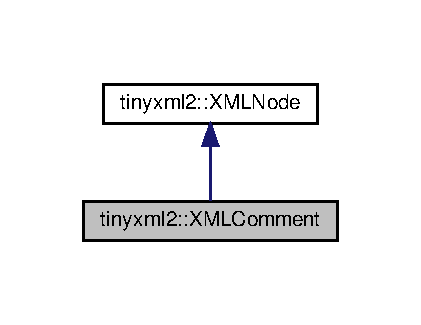
\includegraphics[width=202pt]{classtinyxml2_1_1_x_m_l_comment__inherit__graph}
\end{center}
\end{figure}


Collaboration diagram for tinyxml2\+:\+:X\+M\+L\+Comment\+:
\nopagebreak
\begin{figure}[H]
\begin{center}
\leavevmode
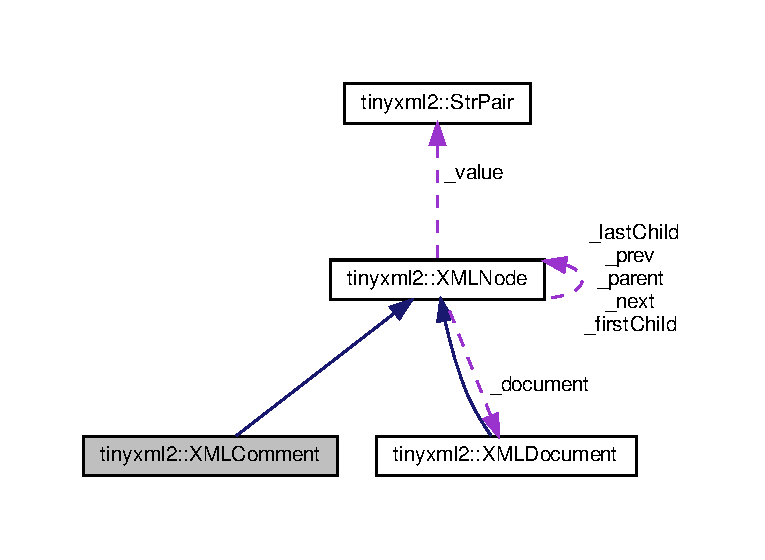
\includegraphics[width=350pt]{classtinyxml2_1_1_x_m_l_comment__coll__graph}
\end{center}
\end{figure}
\subsection*{Public Member Functions}
\begin{DoxyCompactItemize}
\item 
\mbox{\Hypertarget{classtinyxml2_1_1_x_m_l_comment_a8093e1dc8a34fa446d9dc3fde0e6c0ee}\label{classtinyxml2_1_1_x_m_l_comment_a8093e1dc8a34fa446d9dc3fde0e6c0ee}} 
virtual \hyperlink{classtinyxml2_1_1_x_m_l_comment}{X\+M\+L\+Comment} $\ast$ \hyperlink{classtinyxml2_1_1_x_m_l_comment_a8093e1dc8a34fa446d9dc3fde0e6c0ee}{To\+Comment} ()
\begin{DoxyCompactList}\small\item\em Safely cast to a Comment, or null. \end{DoxyCompactList}\item 
\mbox{\Hypertarget{classtinyxml2_1_1_x_m_l_comment_a8e60caf06d8e88876a94b81db026b85c}\label{classtinyxml2_1_1_x_m_l_comment_a8e60caf06d8e88876a94b81db026b85c}} 
virtual const \hyperlink{classtinyxml2_1_1_x_m_l_comment}{X\+M\+L\+Comment} $\ast$ {\bfseries To\+Comment} () const
\item 
virtual bool \hyperlink{classtinyxml2_1_1_x_m_l_comment_a27b37d16cea01b5329dfbbb4f9508e39}{Accept} (\hyperlink{classtinyxml2_1_1_x_m_l_visitor}{X\+M\+L\+Visitor} $\ast$visitor) const
\item 
virtual \hyperlink{classtinyxml2_1_1_x_m_l_node}{X\+M\+L\+Node} $\ast$ \hyperlink{classtinyxml2_1_1_x_m_l_comment_adf5b5c0319351dcc339df098d11e8fb2}{Shallow\+Clone} (\hyperlink{classtinyxml2_1_1_x_m_l_document}{X\+M\+L\+Document} $\ast$document) const
\item 
virtual bool \hyperlink{classtinyxml2_1_1_x_m_l_comment_a965d880a99d58dd915caa88dc37a9b51}{Shallow\+Equal} (const \hyperlink{classtinyxml2_1_1_x_m_l_node}{X\+M\+L\+Node} $\ast$compare) const
\end{DoxyCompactItemize}
\subsection*{Protected Member Functions}
\begin{DoxyCompactItemize}
\item 
\mbox{\Hypertarget{classtinyxml2_1_1_x_m_l_comment_ae6463adc3edd93a8e5a9b2b7e99cdf91}\label{classtinyxml2_1_1_x_m_l_comment_ae6463adc3edd93a8e5a9b2b7e99cdf91}} 
{\bfseries X\+M\+L\+Comment} (\hyperlink{classtinyxml2_1_1_x_m_l_document}{X\+M\+L\+Document} $\ast$doc)
\item 
\mbox{\Hypertarget{classtinyxml2_1_1_x_m_l_comment_a3430281eed8d1023bafa9e633f44f509}\label{classtinyxml2_1_1_x_m_l_comment_a3430281eed8d1023bafa9e633f44f509}} 
char $\ast$ {\bfseries Parse\+Deep} (char $\ast$p, \hyperlink{classtinyxml2_1_1_str_pair}{Str\+Pair} $\ast$parent\+End\+Tag, int $\ast$cur\+Line\+Num\+Ptr)
\end{DoxyCompactItemize}
\subsection*{Friends}
\begin{DoxyCompactItemize}
\item 
\mbox{\Hypertarget{classtinyxml2_1_1_x_m_l_comment_a4eee3bda60c60a30e4e8cd4ea91c4c6e}\label{classtinyxml2_1_1_x_m_l_comment_a4eee3bda60c60a30e4e8cd4ea91c4c6e}} 
class {\bfseries X\+M\+L\+Document}
\end{DoxyCompactItemize}
\subsection*{Additional Inherited Members}


\subsection{Detailed Description}
An X\+ML Comment. 

\subsection{Member Function Documentation}
\mbox{\Hypertarget{classtinyxml2_1_1_x_m_l_comment_a27b37d16cea01b5329dfbbb4f9508e39}\label{classtinyxml2_1_1_x_m_l_comment_a27b37d16cea01b5329dfbbb4f9508e39}} 
\index{tinyxml2\+::\+X\+M\+L\+Comment@{tinyxml2\+::\+X\+M\+L\+Comment}!Accept@{Accept}}
\index{Accept@{Accept}!tinyxml2\+::\+X\+M\+L\+Comment@{tinyxml2\+::\+X\+M\+L\+Comment}}
\subsubsection{\texorpdfstring{Accept()}{Accept()}}
{\footnotesize\ttfamily bool tinyxml2\+::\+X\+M\+L\+Comment\+::\+Accept (\begin{DoxyParamCaption}\item[{\hyperlink{classtinyxml2_1_1_x_m_l_visitor}{X\+M\+L\+Visitor} $\ast$}]{visitor }\end{DoxyParamCaption}) const\hspace{0.3cm}{\ttfamily [virtual]}}

Accept a hierarchical visit of the nodes in the Tiny\+X\+M\+L-\/2 D\+OM. Every node in the X\+ML tree will be conditionally visited and the host will be called back via the \hyperlink{classtinyxml2_1_1_x_m_l_visitor}{X\+M\+L\+Visitor} interface.

This is essentially a S\+AX interface for Tiny\+X\+M\+L-\/2. (Note however it doesn\textquotesingle{}t re-\/parse the X\+ML for the callbacks, so the performance of Tiny\+X\+M\+L-\/2 is unchanged by using this interface versus any other.)

The interface has been based on ideas from\+:


\begin{DoxyItemize}
\item \href{http://www.saxproject.org/}{\tt http\+://www.\+saxproject.\+org/}
\item \href{http://c2.com/cgi/wiki?HierarchicalVisitorPattern}{\tt http\+://c2.\+com/cgi/wiki?\+Hierarchical\+Visitor\+Pattern}
\end{DoxyItemize}

Which are both good references for \char`\"{}visiting\char`\"{}.

An example of using \hyperlink{classtinyxml2_1_1_x_m_l_comment_a27b37d16cea01b5329dfbbb4f9508e39}{Accept()}\+: \begin{DoxyVerb}XMLPrinter printer;
tinyxmlDoc.Accept( &printer );
const char* xmlcstr = printer.CStr();
\end{DoxyVerb}
 

Implements \hyperlink{classtinyxml2_1_1_x_m_l_node_a81e66df0a44c67a7af17f3b77a152785}{tinyxml2\+::\+X\+M\+L\+Node}.

\mbox{\Hypertarget{classtinyxml2_1_1_x_m_l_comment_adf5b5c0319351dcc339df098d11e8fb2}\label{classtinyxml2_1_1_x_m_l_comment_adf5b5c0319351dcc339df098d11e8fb2}} 
\index{tinyxml2\+::\+X\+M\+L\+Comment@{tinyxml2\+::\+X\+M\+L\+Comment}!Shallow\+Clone@{Shallow\+Clone}}
\index{Shallow\+Clone@{Shallow\+Clone}!tinyxml2\+::\+X\+M\+L\+Comment@{tinyxml2\+::\+X\+M\+L\+Comment}}
\subsubsection{\texorpdfstring{Shallow\+Clone()}{ShallowClone()}}
{\footnotesize\ttfamily \hyperlink{classtinyxml2_1_1_x_m_l_node}{X\+M\+L\+Node} $\ast$ tinyxml2\+::\+X\+M\+L\+Comment\+::\+Shallow\+Clone (\begin{DoxyParamCaption}\item[{\hyperlink{classtinyxml2_1_1_x_m_l_document}{X\+M\+L\+Document} $\ast$}]{document }\end{DoxyParamCaption}) const\hspace{0.3cm}{\ttfamily [virtual]}}

Make a copy of this node, but not its children. You may pass in a Document pointer that will be the owner of the new Node. If the \textquotesingle{}document\textquotesingle{} is null, then the node returned will be allocated from the current Document. (this-\/$>$\hyperlink{classtinyxml2_1_1_x_m_l_node_af343d1ef0b45c0020e62d784d7e67a68}{Get\+Document()})

Note\+: if called on a \hyperlink{classtinyxml2_1_1_x_m_l_document}{X\+M\+L\+Document}, this will return null. 

Implements \hyperlink{classtinyxml2_1_1_x_m_l_node_a8402cbd3129d20e9e6024bbcc0531283}{tinyxml2\+::\+X\+M\+L\+Node}.

\mbox{\Hypertarget{classtinyxml2_1_1_x_m_l_comment_a965d880a99d58dd915caa88dc37a9b51}\label{classtinyxml2_1_1_x_m_l_comment_a965d880a99d58dd915caa88dc37a9b51}} 
\index{tinyxml2\+::\+X\+M\+L\+Comment@{tinyxml2\+::\+X\+M\+L\+Comment}!Shallow\+Equal@{Shallow\+Equal}}
\index{Shallow\+Equal@{Shallow\+Equal}!tinyxml2\+::\+X\+M\+L\+Comment@{tinyxml2\+::\+X\+M\+L\+Comment}}
\subsubsection{\texorpdfstring{Shallow\+Equal()}{ShallowEqual()}}
{\footnotesize\ttfamily bool tinyxml2\+::\+X\+M\+L\+Comment\+::\+Shallow\+Equal (\begin{DoxyParamCaption}\item[{const \hyperlink{classtinyxml2_1_1_x_m_l_node}{X\+M\+L\+Node} $\ast$}]{compare }\end{DoxyParamCaption}) const\hspace{0.3cm}{\ttfamily [virtual]}}

Test if 2 nodes are the same, but don\textquotesingle{}t test children. The 2 nodes do not need to be in the same Document.

Note\+: if called on a \hyperlink{classtinyxml2_1_1_x_m_l_document}{X\+M\+L\+Document}, this will return false. 

Implements \hyperlink{classtinyxml2_1_1_x_m_l_node_a7ce18b751c3ea09eac292dca264f9226}{tinyxml2\+::\+X\+M\+L\+Node}.



The documentation for this class was generated from the following files\+:\begin{DoxyCompactItemize}
\item 
/home/ijlee/workspace/sdmt/src/tinyxml2.\+h\item 
/home/ijlee/workspace/sdmt/src/tinyxml2.\+cpp\end{DoxyCompactItemize}

\hypertarget{classtinyxml2_1_1_x_m_l_const_handle}{}\section{tinyxml2\+:\+:X\+M\+L\+Const\+Handle Class Reference}
\label{classtinyxml2_1_1_x_m_l_const_handle}\index{tinyxml2\+::\+X\+M\+L\+Const\+Handle@{tinyxml2\+::\+X\+M\+L\+Const\+Handle}}


{\ttfamily \#include $<$tinyxml2.\+h$>$}

\subsection*{Public Member Functions}
\begin{DoxyCompactItemize}
\item 
\mbox{\Hypertarget{classtinyxml2_1_1_x_m_l_const_handle_a098bda71fa11d7c74ccddab59d5dd534}\label{classtinyxml2_1_1_x_m_l_const_handle_a098bda71fa11d7c74ccddab59d5dd534}} 
{\bfseries X\+M\+L\+Const\+Handle} (const \hyperlink{classtinyxml2_1_1_x_m_l_node}{X\+M\+L\+Node} $\ast$node)
\item 
\mbox{\Hypertarget{classtinyxml2_1_1_x_m_l_const_handle_a8420a0c4720637e0529e78c2e22f2b0b}\label{classtinyxml2_1_1_x_m_l_const_handle_a8420a0c4720637e0529e78c2e22f2b0b}} 
{\bfseries X\+M\+L\+Const\+Handle} (const \hyperlink{classtinyxml2_1_1_x_m_l_node}{X\+M\+L\+Node} \&node)
\item 
\mbox{\Hypertarget{classtinyxml2_1_1_x_m_l_const_handle_a639317ad315ff24f4ef0dc69312d7303}\label{classtinyxml2_1_1_x_m_l_const_handle_a639317ad315ff24f4ef0dc69312d7303}} 
{\bfseries X\+M\+L\+Const\+Handle} (const \hyperlink{classtinyxml2_1_1_x_m_l_const_handle}{X\+M\+L\+Const\+Handle} \&ref)
\item 
\mbox{\Hypertarget{classtinyxml2_1_1_x_m_l_const_handle_a2d74c91df1ff9aa5f9b57e3dceddbf94}\label{classtinyxml2_1_1_x_m_l_const_handle_a2d74c91df1ff9aa5f9b57e3dceddbf94}} 
\hyperlink{classtinyxml2_1_1_x_m_l_const_handle}{X\+M\+L\+Const\+Handle} \& {\bfseries operator=} (const \hyperlink{classtinyxml2_1_1_x_m_l_const_handle}{X\+M\+L\+Const\+Handle} \&ref)
\item 
\mbox{\Hypertarget{classtinyxml2_1_1_x_m_l_const_handle_aef06bd16cb308652a32b864b0a743136}\label{classtinyxml2_1_1_x_m_l_const_handle_aef06bd16cb308652a32b864b0a743136}} 
const \hyperlink{classtinyxml2_1_1_x_m_l_const_handle}{X\+M\+L\+Const\+Handle} {\bfseries First\+Child} () const
\item 
\mbox{\Hypertarget{classtinyxml2_1_1_x_m_l_const_handle_ac747db472ffc55c5af2e82ffec813640}\label{classtinyxml2_1_1_x_m_l_const_handle_ac747db472ffc55c5af2e82ffec813640}} 
const \hyperlink{classtinyxml2_1_1_x_m_l_const_handle}{X\+M\+L\+Const\+Handle} {\bfseries First\+Child\+Element} (const char $\ast$name=0) const
\item 
\mbox{\Hypertarget{classtinyxml2_1_1_x_m_l_const_handle_a908436124990f3d7b35cb7df20d31d9e}\label{classtinyxml2_1_1_x_m_l_const_handle_a908436124990f3d7b35cb7df20d31d9e}} 
const \hyperlink{classtinyxml2_1_1_x_m_l_const_handle}{X\+M\+L\+Const\+Handle} {\bfseries Last\+Child} () const
\item 
\mbox{\Hypertarget{classtinyxml2_1_1_x_m_l_const_handle_a9de0475ec42bd50c0e64624a250ba5b2}\label{classtinyxml2_1_1_x_m_l_const_handle_a9de0475ec42bd50c0e64624a250ba5b2}} 
const \hyperlink{classtinyxml2_1_1_x_m_l_const_handle}{X\+M\+L\+Const\+Handle} {\bfseries Last\+Child\+Element} (const char $\ast$name=0) const
\item 
\mbox{\Hypertarget{classtinyxml2_1_1_x_m_l_const_handle_acf68cc7930e4ac883e0c7e16ef2fbb66}\label{classtinyxml2_1_1_x_m_l_const_handle_acf68cc7930e4ac883e0c7e16ef2fbb66}} 
const \hyperlink{classtinyxml2_1_1_x_m_l_const_handle}{X\+M\+L\+Const\+Handle} {\bfseries Previous\+Sibling} () const
\item 
\mbox{\Hypertarget{classtinyxml2_1_1_x_m_l_const_handle_aef99308659f2617299ac29980769a91e}\label{classtinyxml2_1_1_x_m_l_const_handle_aef99308659f2617299ac29980769a91e}} 
const \hyperlink{classtinyxml2_1_1_x_m_l_const_handle}{X\+M\+L\+Const\+Handle} {\bfseries Previous\+Sibling\+Element} (const char $\ast$name=0) const
\item 
\mbox{\Hypertarget{classtinyxml2_1_1_x_m_l_const_handle_aec3710e455f41014026ef17fbbb0efb3}\label{classtinyxml2_1_1_x_m_l_const_handle_aec3710e455f41014026ef17fbbb0efb3}} 
const \hyperlink{classtinyxml2_1_1_x_m_l_const_handle}{X\+M\+L\+Const\+Handle} {\bfseries Next\+Sibling} () const
\item 
\mbox{\Hypertarget{classtinyxml2_1_1_x_m_l_const_handle_a3c9e6b48b02d3d5232e1e8780753d8a5}\label{classtinyxml2_1_1_x_m_l_const_handle_a3c9e6b48b02d3d5232e1e8780753d8a5}} 
const \hyperlink{classtinyxml2_1_1_x_m_l_const_handle}{X\+M\+L\+Const\+Handle} {\bfseries Next\+Sibling\+Element} (const char $\ast$name=0) const
\item 
\mbox{\Hypertarget{classtinyxml2_1_1_x_m_l_const_handle_a61812760cb08bc1b050e65b73a08457b}\label{classtinyxml2_1_1_x_m_l_const_handle_a61812760cb08bc1b050e65b73a08457b}} 
const \hyperlink{classtinyxml2_1_1_x_m_l_node}{X\+M\+L\+Node} $\ast$ {\bfseries To\+Node} () const
\item 
\mbox{\Hypertarget{classtinyxml2_1_1_x_m_l_const_handle_a4dba53c6e201d412e915620feaaa56f3}\label{classtinyxml2_1_1_x_m_l_const_handle_a4dba53c6e201d412e915620feaaa56f3}} 
const \hyperlink{classtinyxml2_1_1_x_m_l_element}{X\+M\+L\+Element} $\ast$ {\bfseries To\+Element} () const
\item 
\mbox{\Hypertarget{classtinyxml2_1_1_x_m_l_const_handle_a80e24d90d476005aa35602a665358e2d}\label{classtinyxml2_1_1_x_m_l_const_handle_a80e24d90d476005aa35602a665358e2d}} 
const \hyperlink{classtinyxml2_1_1_x_m_l_text}{X\+M\+L\+Text} $\ast$ {\bfseries To\+Text} () const
\item 
\mbox{\Hypertarget{classtinyxml2_1_1_x_m_l_const_handle_a4395e5feaba7b456a81ca274880ea3d3}\label{classtinyxml2_1_1_x_m_l_const_handle_a4395e5feaba7b456a81ca274880ea3d3}} 
const \hyperlink{classtinyxml2_1_1_x_m_l_unknown}{X\+M\+L\+Unknown} $\ast$ {\bfseries To\+Unknown} () const
\item 
\mbox{\Hypertarget{classtinyxml2_1_1_x_m_l_const_handle_a55e306d105fa80d626041e4d3b77b716}\label{classtinyxml2_1_1_x_m_l_const_handle_a55e306d105fa80d626041e4d3b77b716}} 
const \hyperlink{classtinyxml2_1_1_x_m_l_declaration}{X\+M\+L\+Declaration} $\ast$ {\bfseries To\+Declaration} () const
\end{DoxyCompactItemize}


\subsection{Detailed Description}
A variant of the \hyperlink{classtinyxml2_1_1_x_m_l_handle}{X\+M\+L\+Handle} class for working with const X\+M\+L\+Nodes and Documents. It is the same in all regards, except for the \textquotesingle{}const\textquotesingle{} qualifiers. See \hyperlink{classtinyxml2_1_1_x_m_l_handle}{X\+M\+L\+Handle} for A\+PI. 

The documentation for this class was generated from the following file\+:\begin{DoxyCompactItemize}
\item 
/home/ijlee/workspace/sdmt/src/tinyxml2.\+h\end{DoxyCompactItemize}

\hypertarget{classtinyxml2_1_1_x_m_l_declaration}{}\section{tinyxml2\+:\+:X\+M\+L\+Declaration Class Reference}
\label{classtinyxml2_1_1_x_m_l_declaration}\index{tinyxml2\+::\+X\+M\+L\+Declaration@{tinyxml2\+::\+X\+M\+L\+Declaration}}


{\ttfamily \#include $<$tinyxml2.\+h$>$}



Inheritance diagram for tinyxml2\+:\+:X\+M\+L\+Declaration\+:
\nopagebreak
\begin{figure}[H]
\begin{center}
\leavevmode
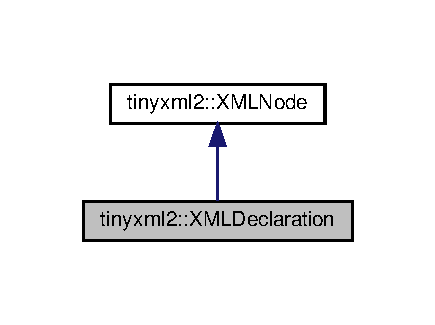
\includegraphics[width=209pt]{classtinyxml2_1_1_x_m_l_declaration__inherit__graph}
\end{center}
\end{figure}


Collaboration diagram for tinyxml2\+:\+:X\+M\+L\+Declaration\+:
\nopagebreak
\begin{figure}[H]
\begin{center}
\leavevmode
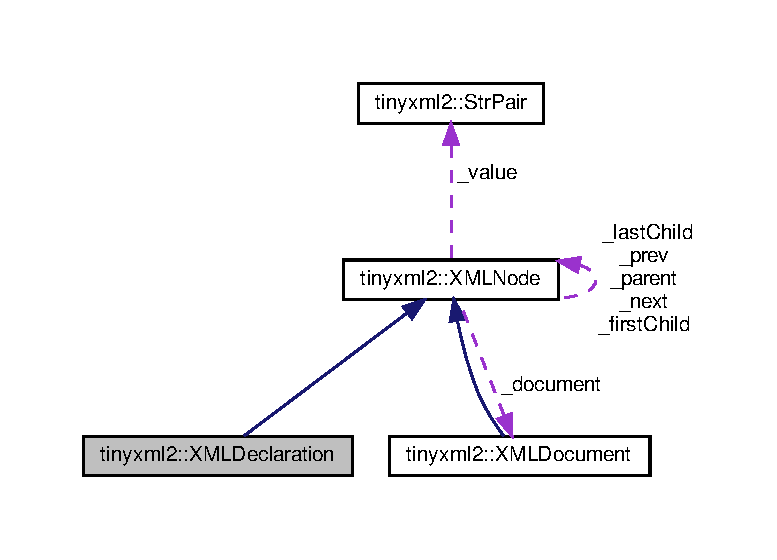
\includegraphics[width=350pt]{classtinyxml2_1_1_x_m_l_declaration__coll__graph}
\end{center}
\end{figure}
\subsection*{Public Member Functions}
\begin{DoxyCompactItemize}
\item 
\mbox{\Hypertarget{classtinyxml2_1_1_x_m_l_declaration_a159d8ac45865215e88059ea1e5b52fc5}\label{classtinyxml2_1_1_x_m_l_declaration_a159d8ac45865215e88059ea1e5b52fc5}} 
virtual \hyperlink{classtinyxml2_1_1_x_m_l_declaration}{X\+M\+L\+Declaration} $\ast$ \hyperlink{classtinyxml2_1_1_x_m_l_declaration_a159d8ac45865215e88059ea1e5b52fc5}{To\+Declaration} ()
\begin{DoxyCompactList}\small\item\em Safely cast to a Declaration, or null. \end{DoxyCompactList}\item 
\mbox{\Hypertarget{classtinyxml2_1_1_x_m_l_declaration_aa20c3315b18c3b88830dccf5c493259b}\label{classtinyxml2_1_1_x_m_l_declaration_aa20c3315b18c3b88830dccf5c493259b}} 
virtual const \hyperlink{classtinyxml2_1_1_x_m_l_declaration}{X\+M\+L\+Declaration} $\ast$ {\bfseries To\+Declaration} () const
\item 
virtual bool \hyperlink{classtinyxml2_1_1_x_m_l_declaration_acf47629d9fc08ed6f1c164a97bcf794b}{Accept} (\hyperlink{classtinyxml2_1_1_x_m_l_visitor}{X\+M\+L\+Visitor} $\ast$visitor) const
\item 
virtual \hyperlink{classtinyxml2_1_1_x_m_l_node}{X\+M\+L\+Node} $\ast$ \hyperlink{classtinyxml2_1_1_x_m_l_declaration_ad9d60e6d2df75c13eb6bf7319985b747}{Shallow\+Clone} (\hyperlink{classtinyxml2_1_1_x_m_l_document}{X\+M\+L\+Document} $\ast$document) const
\item 
virtual bool \hyperlink{classtinyxml2_1_1_x_m_l_declaration_ae8b4d3a399857029f36c322b0801b69c}{Shallow\+Equal} (const \hyperlink{classtinyxml2_1_1_x_m_l_node}{X\+M\+L\+Node} $\ast$compare) const
\end{DoxyCompactItemize}
\subsection*{Protected Member Functions}
\begin{DoxyCompactItemize}
\item 
\mbox{\Hypertarget{classtinyxml2_1_1_x_m_l_declaration_aef9586f2ce5df5feba74dde49a242b06}\label{classtinyxml2_1_1_x_m_l_declaration_aef9586f2ce5df5feba74dde49a242b06}} 
{\bfseries X\+M\+L\+Declaration} (\hyperlink{classtinyxml2_1_1_x_m_l_document}{X\+M\+L\+Document} $\ast$doc)
\item 
\mbox{\Hypertarget{classtinyxml2_1_1_x_m_l_declaration_a42a2a36f4d78dc745063b79c16538b9b}\label{classtinyxml2_1_1_x_m_l_declaration_a42a2a36f4d78dc745063b79c16538b9b}} 
char $\ast$ {\bfseries Parse\+Deep} (char $\ast$p, \hyperlink{classtinyxml2_1_1_str_pair}{Str\+Pair} $\ast$parent\+End\+Tag, int $\ast$cur\+Line\+Num\+Ptr)
\end{DoxyCompactItemize}
\subsection*{Friends}
\begin{DoxyCompactItemize}
\item 
\mbox{\Hypertarget{classtinyxml2_1_1_x_m_l_declaration_a4eee3bda60c60a30e4e8cd4ea91c4c6e}\label{classtinyxml2_1_1_x_m_l_declaration_a4eee3bda60c60a30e4e8cd4ea91c4c6e}} 
class {\bfseries X\+M\+L\+Document}
\end{DoxyCompactItemize}
\subsection*{Additional Inherited Members}


\subsection{Detailed Description}
In correct X\+ML the declaration is the first entry in the file. \begin{DoxyVerb}    <?xml version="1.0" standalone="yes"?>
\end{DoxyVerb}


Tiny\+X\+M\+L-\/2 will happily read or write files without a declaration, however.

The text of the declaration isn\textquotesingle{}t interpreted. It is parsed and written as a string. 

\subsection{Member Function Documentation}
\mbox{\Hypertarget{classtinyxml2_1_1_x_m_l_declaration_acf47629d9fc08ed6f1c164a97bcf794b}\label{classtinyxml2_1_1_x_m_l_declaration_acf47629d9fc08ed6f1c164a97bcf794b}} 
\index{tinyxml2\+::\+X\+M\+L\+Declaration@{tinyxml2\+::\+X\+M\+L\+Declaration}!Accept@{Accept}}
\index{Accept@{Accept}!tinyxml2\+::\+X\+M\+L\+Declaration@{tinyxml2\+::\+X\+M\+L\+Declaration}}
\subsubsection{\texorpdfstring{Accept()}{Accept()}}
{\footnotesize\ttfamily bool tinyxml2\+::\+X\+M\+L\+Declaration\+::\+Accept (\begin{DoxyParamCaption}\item[{\hyperlink{classtinyxml2_1_1_x_m_l_visitor}{X\+M\+L\+Visitor} $\ast$}]{visitor }\end{DoxyParamCaption}) const\hspace{0.3cm}{\ttfamily [virtual]}}

Accept a hierarchical visit of the nodes in the Tiny\+X\+M\+L-\/2 D\+OM. Every node in the X\+ML tree will be conditionally visited and the host will be called back via the \hyperlink{classtinyxml2_1_1_x_m_l_visitor}{X\+M\+L\+Visitor} interface.

This is essentially a S\+AX interface for Tiny\+X\+M\+L-\/2. (Note however it doesn\textquotesingle{}t re-\/parse the X\+ML for the callbacks, so the performance of Tiny\+X\+M\+L-\/2 is unchanged by using this interface versus any other.)

The interface has been based on ideas from\+:


\begin{DoxyItemize}
\item \href{http://www.saxproject.org/}{\tt http\+://www.\+saxproject.\+org/}
\item \href{http://c2.com/cgi/wiki?HierarchicalVisitorPattern}{\tt http\+://c2.\+com/cgi/wiki?\+Hierarchical\+Visitor\+Pattern}
\end{DoxyItemize}

Which are both good references for \char`\"{}visiting\char`\"{}.

An example of using \hyperlink{classtinyxml2_1_1_x_m_l_declaration_acf47629d9fc08ed6f1c164a97bcf794b}{Accept()}\+: \begin{DoxyVerb}XMLPrinter printer;
tinyxmlDoc.Accept( &printer );
const char* xmlcstr = printer.CStr();
\end{DoxyVerb}
 

Implements \hyperlink{classtinyxml2_1_1_x_m_l_node_a81e66df0a44c67a7af17f3b77a152785}{tinyxml2\+::\+X\+M\+L\+Node}.

\mbox{\Hypertarget{classtinyxml2_1_1_x_m_l_declaration_ad9d60e6d2df75c13eb6bf7319985b747}\label{classtinyxml2_1_1_x_m_l_declaration_ad9d60e6d2df75c13eb6bf7319985b747}} 
\index{tinyxml2\+::\+X\+M\+L\+Declaration@{tinyxml2\+::\+X\+M\+L\+Declaration}!Shallow\+Clone@{Shallow\+Clone}}
\index{Shallow\+Clone@{Shallow\+Clone}!tinyxml2\+::\+X\+M\+L\+Declaration@{tinyxml2\+::\+X\+M\+L\+Declaration}}
\subsubsection{\texorpdfstring{Shallow\+Clone()}{ShallowClone()}}
{\footnotesize\ttfamily \hyperlink{classtinyxml2_1_1_x_m_l_node}{X\+M\+L\+Node} $\ast$ tinyxml2\+::\+X\+M\+L\+Declaration\+::\+Shallow\+Clone (\begin{DoxyParamCaption}\item[{\hyperlink{classtinyxml2_1_1_x_m_l_document}{X\+M\+L\+Document} $\ast$}]{document }\end{DoxyParamCaption}) const\hspace{0.3cm}{\ttfamily [virtual]}}

Make a copy of this node, but not its children. You may pass in a Document pointer that will be the owner of the new Node. If the \textquotesingle{}document\textquotesingle{} is null, then the node returned will be allocated from the current Document. (this-\/$>$\hyperlink{classtinyxml2_1_1_x_m_l_node_af343d1ef0b45c0020e62d784d7e67a68}{Get\+Document()})

Note\+: if called on a \hyperlink{classtinyxml2_1_1_x_m_l_document}{X\+M\+L\+Document}, this will return null. 

Implements \hyperlink{classtinyxml2_1_1_x_m_l_node_a8402cbd3129d20e9e6024bbcc0531283}{tinyxml2\+::\+X\+M\+L\+Node}.

\mbox{\Hypertarget{classtinyxml2_1_1_x_m_l_declaration_ae8b4d3a399857029f36c322b0801b69c}\label{classtinyxml2_1_1_x_m_l_declaration_ae8b4d3a399857029f36c322b0801b69c}} 
\index{tinyxml2\+::\+X\+M\+L\+Declaration@{tinyxml2\+::\+X\+M\+L\+Declaration}!Shallow\+Equal@{Shallow\+Equal}}
\index{Shallow\+Equal@{Shallow\+Equal}!tinyxml2\+::\+X\+M\+L\+Declaration@{tinyxml2\+::\+X\+M\+L\+Declaration}}
\subsubsection{\texorpdfstring{Shallow\+Equal()}{ShallowEqual()}}
{\footnotesize\ttfamily bool tinyxml2\+::\+X\+M\+L\+Declaration\+::\+Shallow\+Equal (\begin{DoxyParamCaption}\item[{const \hyperlink{classtinyxml2_1_1_x_m_l_node}{X\+M\+L\+Node} $\ast$}]{compare }\end{DoxyParamCaption}) const\hspace{0.3cm}{\ttfamily [virtual]}}

Test if 2 nodes are the same, but don\textquotesingle{}t test children. The 2 nodes do not need to be in the same Document.

Note\+: if called on a \hyperlink{classtinyxml2_1_1_x_m_l_document}{X\+M\+L\+Document}, this will return false. 

Implements \hyperlink{classtinyxml2_1_1_x_m_l_node_a7ce18b751c3ea09eac292dca264f9226}{tinyxml2\+::\+X\+M\+L\+Node}.



The documentation for this class was generated from the following files\+:\begin{DoxyCompactItemize}
\item 
/home/ijlee/workspace/sdmt/src/tinyxml2.\+h\item 
/home/ijlee/workspace/sdmt/src/tinyxml2.\+cpp\end{DoxyCompactItemize}

\hypertarget{classtinyxml2_1_1_x_m_l_document}{}\section{tinyxml2\+:\+:X\+M\+L\+Document Class Reference}
\label{classtinyxml2_1_1_x_m_l_document}\index{tinyxml2\+::\+X\+M\+L\+Document@{tinyxml2\+::\+X\+M\+L\+Document}}


{\ttfamily \#include $<$tinyxml2.\+h$>$}



Inheritance diagram for tinyxml2\+:\+:X\+M\+L\+Document\+:
\nopagebreak
\begin{figure}[H]
\begin{center}
\leavevmode
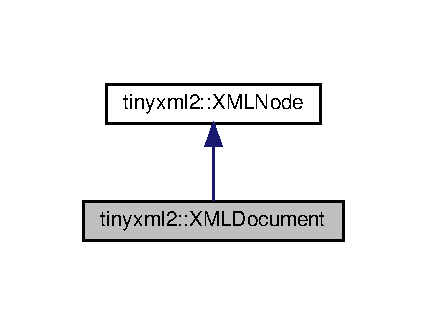
\includegraphics[width=205pt]{classtinyxml2_1_1_x_m_l_document__inherit__graph}
\end{center}
\end{figure}


Collaboration diagram for tinyxml2\+:\+:X\+M\+L\+Document\+:
\nopagebreak
\begin{figure}[H]
\begin{center}
\leavevmode
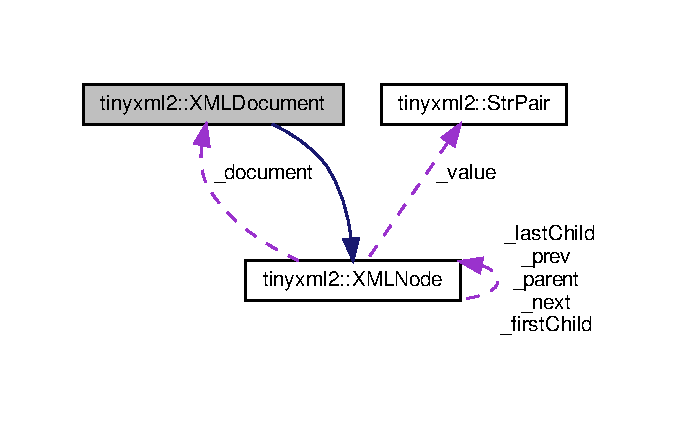
\includegraphics[width=326pt]{classtinyxml2_1_1_x_m_l_document__coll__graph}
\end{center}
\end{figure}
\subsection*{Public Member Functions}
\begin{DoxyCompactItemize}
\item 
\mbox{\Hypertarget{classtinyxml2_1_1_x_m_l_document_a57ddf17b6e054dda10af98991b1b8f70}\label{classtinyxml2_1_1_x_m_l_document_a57ddf17b6e054dda10af98991b1b8f70}} 
\hyperlink{classtinyxml2_1_1_x_m_l_document_a57ddf17b6e054dda10af98991b1b8f70}{X\+M\+L\+Document} (bool process\+Entities=true, Whitespace whitespace\+Mode=P\+R\+E\+S\+E\+R\+V\+E\+\_\+\+W\+H\+I\+T\+E\+S\+P\+A\+CE)
\begin{DoxyCompactList}\small\item\em constructor \end{DoxyCompactList}\item 
\mbox{\Hypertarget{classtinyxml2_1_1_x_m_l_document_a3e185f880882bd978367bb55937735ec}\label{classtinyxml2_1_1_x_m_l_document_a3e185f880882bd978367bb55937735ec}} 
virtual \hyperlink{classtinyxml2_1_1_x_m_l_document}{X\+M\+L\+Document} $\ast$ \hyperlink{classtinyxml2_1_1_x_m_l_document_a3e185f880882bd978367bb55937735ec}{To\+Document} ()
\begin{DoxyCompactList}\small\item\em Safely cast to a Document, or null. \end{DoxyCompactList}\item 
\mbox{\Hypertarget{classtinyxml2_1_1_x_m_l_document_a747ab173887d969fe313b4617f968e99}\label{classtinyxml2_1_1_x_m_l_document_a747ab173887d969fe313b4617f968e99}} 
virtual const \hyperlink{classtinyxml2_1_1_x_m_l_document}{X\+M\+L\+Document} $\ast$ {\bfseries To\+Document} () const
\item 
X\+M\+L\+Error \hyperlink{classtinyxml2_1_1_x_m_l_document_af2b616169e6517182f6725f2498e9a01}{Parse} (const char $\ast$xml, size\+\_\+t n\+Bytes=static\+\_\+cast$<$ size\+\_\+t $>$(-\/1))
\item 
X\+M\+L\+Error \hyperlink{classtinyxml2_1_1_x_m_l_document_a2ebd4647a8af5fc6831b294ac26a150a}{Load\+File} (const char $\ast$filename)
\item 
X\+M\+L\+Error \hyperlink{classtinyxml2_1_1_x_m_l_document_a5f1d330fad44c52f3d265338dd2a6dc2}{Load\+File} (F\+I\+LE $\ast$)
\item 
X\+M\+L\+Error \hyperlink{classtinyxml2_1_1_x_m_l_document_a73ac416b4a2aa0952e841220eb3da18f}{Save\+File} (const char $\ast$filename, bool compact=false)
\item 
X\+M\+L\+Error \hyperlink{classtinyxml2_1_1_x_m_l_document_a8b95779479a0035acc67b3a61dfe1b74}{Save\+File} (F\+I\+LE $\ast$fp, bool compact=false)
\item 
\mbox{\Hypertarget{classtinyxml2_1_1_x_m_l_document_a53e6c035b1b539563fef8c817fb30469}\label{classtinyxml2_1_1_x_m_l_document_a53e6c035b1b539563fef8c817fb30469}} 
bool {\bfseries Process\+Entities} () const
\item 
\mbox{\Hypertarget{classtinyxml2_1_1_x_m_l_document_a810ce508e6e0365497c2a9deb83c9ca7}\label{classtinyxml2_1_1_x_m_l_document_a810ce508e6e0365497c2a9deb83c9ca7}} 
Whitespace {\bfseries Whitespace\+Mode} () const
\item 
bool \hyperlink{classtinyxml2_1_1_x_m_l_document_a33fc5d159db873a179fa26338adb05bd}{Has\+B\+OM} () const
\item 
void \hyperlink{classtinyxml2_1_1_x_m_l_document_a14419b698f7c4b140df4e80f3f0c93b0}{Set\+B\+OM} (bool use\+B\+OM)
\item 
\hyperlink{classtinyxml2_1_1_x_m_l_element}{X\+M\+L\+Element} $\ast$ \hyperlink{classtinyxml2_1_1_x_m_l_document_ad2b70320d3c2a071c2f36928edff3e1c}{Root\+Element} ()
\item 
\mbox{\Hypertarget{classtinyxml2_1_1_x_m_l_document_a2be8ef9d6346bdef34311f91529afae4}\label{classtinyxml2_1_1_x_m_l_document_a2be8ef9d6346bdef34311f91529afae4}} 
const \hyperlink{classtinyxml2_1_1_x_m_l_element}{X\+M\+L\+Element} $\ast$ {\bfseries Root\+Element} () const
\item 
void \hyperlink{classtinyxml2_1_1_x_m_l_document_a867cf5fa3e3ff6ae4847a8b7ee8ec083}{Print} (\hyperlink{classtinyxml2_1_1_x_m_l_printer}{X\+M\+L\+Printer} $\ast$streamer=0) const
\item 
virtual bool \hyperlink{classtinyxml2_1_1_x_m_l_document_ab7be651917a35ab1ff0e4e6d4e565cdf}{Accept} (\hyperlink{classtinyxml2_1_1_x_m_l_visitor}{X\+M\+L\+Visitor} $\ast$visitor) const
\item 
\hyperlink{classtinyxml2_1_1_x_m_l_element}{X\+M\+L\+Element} $\ast$ \hyperlink{classtinyxml2_1_1_x_m_l_document_a3c335a700a43d7c363a393142a23f234}{New\+Element} (const char $\ast$name)
\item 
\hyperlink{classtinyxml2_1_1_x_m_l_comment}{X\+M\+L\+Comment} $\ast$ \hyperlink{classtinyxml2_1_1_x_m_l_document_a386df0befd06aadb5e0cd21381aa955a}{New\+Comment} (const char $\ast$comment)
\item 
\hyperlink{classtinyxml2_1_1_x_m_l_text}{X\+M\+L\+Text} $\ast$ \hyperlink{classtinyxml2_1_1_x_m_l_document_acece5de77a0819f2341b08c1e1ed9987}{New\+Text} (const char $\ast$text)
\item 
\hyperlink{classtinyxml2_1_1_x_m_l_declaration}{X\+M\+L\+Declaration} $\ast$ \hyperlink{classtinyxml2_1_1_x_m_l_document_ae519030c0262fa2daff8993681990e16}{New\+Declaration} (const char $\ast$text=0)
\item 
\hyperlink{classtinyxml2_1_1_x_m_l_unknown}{X\+M\+L\+Unknown} $\ast$ \hyperlink{classtinyxml2_1_1_x_m_l_document_a4954f502c5fd7f49de54c3c0c99bb73d}{New\+Unknown} (const char $\ast$text)
\item 
void \hyperlink{classtinyxml2_1_1_x_m_l_document_ac1d6e2c7fcc1a660624ac4f68e96380d}{Delete\+Node} (\hyperlink{classtinyxml2_1_1_x_m_l_node}{X\+M\+L\+Node} $\ast$node)
\item 
\mbox{\Hypertarget{classtinyxml2_1_1_x_m_l_document_a4085d9c52f1d93214311459d6d1fcf17}\label{classtinyxml2_1_1_x_m_l_document_a4085d9c52f1d93214311459d6d1fcf17}} 
void {\bfseries Clear\+Error} ()
\item 
\mbox{\Hypertarget{classtinyxml2_1_1_x_m_l_document_a34e6318e182e40e3cc4f4ba5d59ed9ed}\label{classtinyxml2_1_1_x_m_l_document_a34e6318e182e40e3cc4f4ba5d59ed9ed}} 
bool \hyperlink{classtinyxml2_1_1_x_m_l_document_a34e6318e182e40e3cc4f4ba5d59ed9ed}{Error} () const
\begin{DoxyCompactList}\small\item\em Return true if there was an error parsing the document. \end{DoxyCompactList}\item 
\mbox{\Hypertarget{classtinyxml2_1_1_x_m_l_document_afa3ed33b3107f920ec2b301f805ac17d}\label{classtinyxml2_1_1_x_m_l_document_afa3ed33b3107f920ec2b301f805ac17d}} 
X\+M\+L\+Error \hyperlink{classtinyxml2_1_1_x_m_l_document_afa3ed33b3107f920ec2b301f805ac17d}{Error\+ID} () const
\begin{DoxyCompactList}\small\item\em Return the error\+ID. \end{DoxyCompactList}\item 
\mbox{\Hypertarget{classtinyxml2_1_1_x_m_l_document_a1a5f2b63427caffd4cde15781d9d11f9}\label{classtinyxml2_1_1_x_m_l_document_a1a5f2b63427caffd4cde15781d9d11f9}} 
const char $\ast$ {\bfseries Error\+Name} () const
\item 
const char $\ast$ \hyperlink{classtinyxml2_1_1_x_m_l_document_ae97fff2402a0d01e0509c430b37996b3}{Error\+Str} () const
\item 
\mbox{\Hypertarget{classtinyxml2_1_1_x_m_l_document_a1d033945b42e125d933d6231e4571552}\label{classtinyxml2_1_1_x_m_l_document_a1d033945b42e125d933d6231e4571552}} 
void \hyperlink{classtinyxml2_1_1_x_m_l_document_a1d033945b42e125d933d6231e4571552}{Print\+Error} () const
\begin{DoxyCompactList}\small\item\em A (trivial) utility function that prints the \hyperlink{classtinyxml2_1_1_x_m_l_document_ae97fff2402a0d01e0509c430b37996b3}{Error\+Str()} to stdout. \end{DoxyCompactList}\item 
\mbox{\Hypertarget{classtinyxml2_1_1_x_m_l_document_a57400f816dbe7799ece33615ead9ab76}\label{classtinyxml2_1_1_x_m_l_document_a57400f816dbe7799ece33615ead9ab76}} 
int \hyperlink{classtinyxml2_1_1_x_m_l_document_a57400f816dbe7799ece33615ead9ab76}{Error\+Line\+Num} () const
\begin{DoxyCompactList}\small\item\em Return the line where the error occurred, or zero if unknown. \end{DoxyCompactList}\item 
\mbox{\Hypertarget{classtinyxml2_1_1_x_m_l_document_a65656b0b2cbc822708eb351504178aaf}\label{classtinyxml2_1_1_x_m_l_document_a65656b0b2cbc822708eb351504178aaf}} 
void \hyperlink{classtinyxml2_1_1_x_m_l_document_a65656b0b2cbc822708eb351504178aaf}{Clear} ()
\begin{DoxyCompactList}\small\item\em Clear the document, resetting it to the initial state. \end{DoxyCompactList}\item 
void \hyperlink{classtinyxml2_1_1_x_m_l_document_af592ffc91514e25a39664521ac83db45}{Deep\+Copy} (\hyperlink{classtinyxml2_1_1_x_m_l_document}{X\+M\+L\+Document} $\ast$target) const
\item 
\mbox{\Hypertarget{classtinyxml2_1_1_x_m_l_document_a25827d1bec509ad566a107e5853ed040}\label{classtinyxml2_1_1_x_m_l_document_a25827d1bec509ad566a107e5853ed040}} 
char $\ast$ {\bfseries Identify} (char $\ast$p, \hyperlink{classtinyxml2_1_1_x_m_l_node}{X\+M\+L\+Node} $\ast$$\ast$node)
\item 
\mbox{\Hypertarget{classtinyxml2_1_1_x_m_l_document_a95d28ecb4760a994556b0a51690b21be}\label{classtinyxml2_1_1_x_m_l_document_a95d28ecb4760a994556b0a51690b21be}} 
void {\bfseries Mark\+In\+Use} (\hyperlink{classtinyxml2_1_1_x_m_l_node}{X\+M\+L\+Node} $\ast$)
\item 
virtual \hyperlink{classtinyxml2_1_1_x_m_l_node}{X\+M\+L\+Node} $\ast$ \hyperlink{classtinyxml2_1_1_x_m_l_document_aa37cc1709d7e1e988bc17dcfb24a69b8}{Shallow\+Clone} (\hyperlink{classtinyxml2_1_1_x_m_l_document}{X\+M\+L\+Document} $\ast$) const
\item 
virtual bool \hyperlink{classtinyxml2_1_1_x_m_l_document_a6fe5ef18699091844fcf64b56ffa5bf9}{Shallow\+Equal} (const \hyperlink{classtinyxml2_1_1_x_m_l_node}{X\+M\+L\+Node} $\ast$) const
\end{DoxyCompactItemize}
\subsection*{Static Public Member Functions}
\begin{DoxyCompactItemize}
\item 
\mbox{\Hypertarget{classtinyxml2_1_1_x_m_l_document_a639f7c295c38dc5a4aafeb2fff93da03}\label{classtinyxml2_1_1_x_m_l_document_a639f7c295c38dc5a4aafeb2fff93da03}} 
static const char $\ast$ {\bfseries Error\+I\+D\+To\+Name} (X\+M\+L\+Error error\+ID)
\end{DoxyCompactItemize}
\subsection*{Friends}
\begin{DoxyCompactItemize}
\item 
\mbox{\Hypertarget{classtinyxml2_1_1_x_m_l_document_ac2fba9b6e452829dd892f7392c24e0eb}\label{classtinyxml2_1_1_x_m_l_document_ac2fba9b6e452829dd892f7392c24e0eb}} 
class {\bfseries X\+M\+L\+Element}
\item 
\mbox{\Hypertarget{classtinyxml2_1_1_x_m_l_document_a8233f9dc4d61d90e93be2a3647c6d957}\label{classtinyxml2_1_1_x_m_l_document_a8233f9dc4d61d90e93be2a3647c6d957}} 
class {\bfseries X\+M\+L\+Node}
\item 
\mbox{\Hypertarget{classtinyxml2_1_1_x_m_l_document_ae50b59416e98bbe7e4bc87df40092109}\label{classtinyxml2_1_1_x_m_l_document_ae50b59416e98bbe7e4bc87df40092109}} 
class {\bfseries X\+M\+L\+Text}
\item 
\mbox{\Hypertarget{classtinyxml2_1_1_x_m_l_document_acee9e261162d4236fb2c30312c54cd4c}\label{classtinyxml2_1_1_x_m_l_document_acee9e261162d4236fb2c30312c54cd4c}} 
class {\bfseries X\+M\+L\+Comment}
\item 
\mbox{\Hypertarget{classtinyxml2_1_1_x_m_l_document_a93d2c2c2db3973083b7d6e7f6f358160}\label{classtinyxml2_1_1_x_m_l_document_a93d2c2c2db3973083b7d6e7f6f358160}} 
class {\bfseries X\+M\+L\+Declaration}
\item 
\mbox{\Hypertarget{classtinyxml2_1_1_x_m_l_document_a6946948274f7a02f5e69b5dbeaea9b35}\label{classtinyxml2_1_1_x_m_l_document_a6946948274f7a02f5e69b5dbeaea9b35}} 
class {\bfseries X\+M\+L\+Unknown}
\end{DoxyCompactItemize}
\subsection*{Additional Inherited Members}


\subsection{Detailed Description}
A Document binds together all the functionality. It can be saved, loaded, and printed to the screen. All Nodes are connected and allocated to a Document. If the Document is deleted, all its Nodes are also deleted. 

\subsection{Member Function Documentation}
\mbox{\Hypertarget{classtinyxml2_1_1_x_m_l_document_ab7be651917a35ab1ff0e4e6d4e565cdf}\label{classtinyxml2_1_1_x_m_l_document_ab7be651917a35ab1ff0e4e6d4e565cdf}} 
\index{tinyxml2\+::\+X\+M\+L\+Document@{tinyxml2\+::\+X\+M\+L\+Document}!Accept@{Accept}}
\index{Accept@{Accept}!tinyxml2\+::\+X\+M\+L\+Document@{tinyxml2\+::\+X\+M\+L\+Document}}
\subsubsection{\texorpdfstring{Accept()}{Accept()}}
{\footnotesize\ttfamily bool tinyxml2\+::\+X\+M\+L\+Document\+::\+Accept (\begin{DoxyParamCaption}\item[{\hyperlink{classtinyxml2_1_1_x_m_l_visitor}{X\+M\+L\+Visitor} $\ast$}]{visitor }\end{DoxyParamCaption}) const\hspace{0.3cm}{\ttfamily [virtual]}}

Accept a hierarchical visit of the nodes in the Tiny\+X\+M\+L-\/2 D\+OM. Every node in the X\+ML tree will be conditionally visited and the host will be called back via the \hyperlink{classtinyxml2_1_1_x_m_l_visitor}{X\+M\+L\+Visitor} interface.

This is essentially a S\+AX interface for Tiny\+X\+M\+L-\/2. (Note however it doesn\textquotesingle{}t re-\/parse the X\+ML for the callbacks, so the performance of Tiny\+X\+M\+L-\/2 is unchanged by using this interface versus any other.)

The interface has been based on ideas from\+:


\begin{DoxyItemize}
\item \href{http://www.saxproject.org/}{\tt http\+://www.\+saxproject.\+org/}
\item \href{http://c2.com/cgi/wiki?HierarchicalVisitorPattern}{\tt http\+://c2.\+com/cgi/wiki?\+Hierarchical\+Visitor\+Pattern}
\end{DoxyItemize}

Which are both good references for \char`\"{}visiting\char`\"{}.

An example of using \hyperlink{classtinyxml2_1_1_x_m_l_document_ab7be651917a35ab1ff0e4e6d4e565cdf}{Accept()}\+: \begin{DoxyVerb}XMLPrinter printer;
tinyxmlDoc.Accept( &printer );
const char* xmlcstr = printer.CStr();
\end{DoxyVerb}
 

Implements \hyperlink{classtinyxml2_1_1_x_m_l_node_a81e66df0a44c67a7af17f3b77a152785}{tinyxml2\+::\+X\+M\+L\+Node}.

\mbox{\Hypertarget{classtinyxml2_1_1_x_m_l_document_af592ffc91514e25a39664521ac83db45}\label{classtinyxml2_1_1_x_m_l_document_af592ffc91514e25a39664521ac83db45}} 
\index{tinyxml2\+::\+X\+M\+L\+Document@{tinyxml2\+::\+X\+M\+L\+Document}!Deep\+Copy@{Deep\+Copy}}
\index{Deep\+Copy@{Deep\+Copy}!tinyxml2\+::\+X\+M\+L\+Document@{tinyxml2\+::\+X\+M\+L\+Document}}
\subsubsection{\texorpdfstring{Deep\+Copy()}{DeepCopy()}}
{\footnotesize\ttfamily void tinyxml2\+::\+X\+M\+L\+Document\+::\+Deep\+Copy (\begin{DoxyParamCaption}\item[{\hyperlink{classtinyxml2_1_1_x_m_l_document}{X\+M\+L\+Document} $\ast$}]{target }\end{DoxyParamCaption}) const}

Copies this document to a target document. The target will be completely cleared before the copy. If you want to copy a sub-\/tree, see \hyperlink{classtinyxml2_1_1_x_m_l_node_a3bb369fd733f1989b751d99a9417adab}{X\+M\+L\+Node\+::\+Deep\+Clone()}.

N\+O\+TE\+: that the \textquotesingle{}target\textquotesingle{} must be non-\/null. \mbox{\Hypertarget{classtinyxml2_1_1_x_m_l_document_ac1d6e2c7fcc1a660624ac4f68e96380d}\label{classtinyxml2_1_1_x_m_l_document_ac1d6e2c7fcc1a660624ac4f68e96380d}} 
\index{tinyxml2\+::\+X\+M\+L\+Document@{tinyxml2\+::\+X\+M\+L\+Document}!Delete\+Node@{Delete\+Node}}
\index{Delete\+Node@{Delete\+Node}!tinyxml2\+::\+X\+M\+L\+Document@{tinyxml2\+::\+X\+M\+L\+Document}}
\subsubsection{\texorpdfstring{Delete\+Node()}{DeleteNode()}}
{\footnotesize\ttfamily void tinyxml2\+::\+X\+M\+L\+Document\+::\+Delete\+Node (\begin{DoxyParamCaption}\item[{\hyperlink{classtinyxml2_1_1_x_m_l_node}{X\+M\+L\+Node} $\ast$}]{node }\end{DoxyParamCaption})}

Delete a node associated with this document. It will be unlinked from the D\+OM. \mbox{\Hypertarget{classtinyxml2_1_1_x_m_l_document_ae97fff2402a0d01e0509c430b37996b3}\label{classtinyxml2_1_1_x_m_l_document_ae97fff2402a0d01e0509c430b37996b3}} 
\index{tinyxml2\+::\+X\+M\+L\+Document@{tinyxml2\+::\+X\+M\+L\+Document}!Error\+Str@{Error\+Str}}
\index{Error\+Str@{Error\+Str}!tinyxml2\+::\+X\+M\+L\+Document@{tinyxml2\+::\+X\+M\+L\+Document}}
\subsubsection{\texorpdfstring{Error\+Str()}{ErrorStr()}}
{\footnotesize\ttfamily const char $\ast$ tinyxml2\+::\+X\+M\+L\+Document\+::\+Error\+Str (\begin{DoxyParamCaption}{ }\end{DoxyParamCaption}) const}

Returns a \char`\"{}long form\char`\"{} error description. A hopefully helpful diagnostic with location, line number, and/or additional info. \mbox{\Hypertarget{classtinyxml2_1_1_x_m_l_document_a33fc5d159db873a179fa26338adb05bd}\label{classtinyxml2_1_1_x_m_l_document_a33fc5d159db873a179fa26338adb05bd}} 
\index{tinyxml2\+::\+X\+M\+L\+Document@{tinyxml2\+::\+X\+M\+L\+Document}!Has\+B\+OM@{Has\+B\+OM}}
\index{Has\+B\+OM@{Has\+B\+OM}!tinyxml2\+::\+X\+M\+L\+Document@{tinyxml2\+::\+X\+M\+L\+Document}}
\subsubsection{\texorpdfstring{Has\+B\+O\+M()}{HasBOM()}}
{\footnotesize\ttfamily bool tinyxml2\+::\+X\+M\+L\+Document\+::\+Has\+B\+OM (\begin{DoxyParamCaption}{ }\end{DoxyParamCaption}) const\hspace{0.3cm}{\ttfamily [inline]}}

Returns true if this document has a leading Byte Order Mark of U\+T\+F8. \mbox{\Hypertarget{classtinyxml2_1_1_x_m_l_document_a2ebd4647a8af5fc6831b294ac26a150a}\label{classtinyxml2_1_1_x_m_l_document_a2ebd4647a8af5fc6831b294ac26a150a}} 
\index{tinyxml2\+::\+X\+M\+L\+Document@{tinyxml2\+::\+X\+M\+L\+Document}!Load\+File@{Load\+File}}
\index{Load\+File@{Load\+File}!tinyxml2\+::\+X\+M\+L\+Document@{tinyxml2\+::\+X\+M\+L\+Document}}
\subsubsection{\texorpdfstring{Load\+File()}{LoadFile()}\hspace{0.1cm}{\footnotesize\ttfamily [1/2]}}
{\footnotesize\ttfamily X\+M\+L\+Error tinyxml2\+::\+X\+M\+L\+Document\+::\+Load\+File (\begin{DoxyParamCaption}\item[{const char $\ast$}]{filename }\end{DoxyParamCaption})}

Load an X\+ML file from disk. Returns X\+M\+L\+\_\+\+S\+U\+C\+C\+E\+SS (0) on success, or an error\+ID. \mbox{\Hypertarget{classtinyxml2_1_1_x_m_l_document_a5f1d330fad44c52f3d265338dd2a6dc2}\label{classtinyxml2_1_1_x_m_l_document_a5f1d330fad44c52f3d265338dd2a6dc2}} 
\index{tinyxml2\+::\+X\+M\+L\+Document@{tinyxml2\+::\+X\+M\+L\+Document}!Load\+File@{Load\+File}}
\index{Load\+File@{Load\+File}!tinyxml2\+::\+X\+M\+L\+Document@{tinyxml2\+::\+X\+M\+L\+Document}}
\subsubsection{\texorpdfstring{Load\+File()}{LoadFile()}\hspace{0.1cm}{\footnotesize\ttfamily [2/2]}}
{\footnotesize\ttfamily X\+M\+L\+Error tinyxml2\+::\+X\+M\+L\+Document\+::\+Load\+File (\begin{DoxyParamCaption}\item[{F\+I\+LE $\ast$}]{fp }\end{DoxyParamCaption})}

Load an X\+ML file from disk. You are responsible for providing and closing the F\+I\+L\+E$\ast$.

N\+O\+TE\+: The file should be opened as binary (\char`\"{}rb\char`\"{}) not text in order for Tiny\+X\+M\+L-\/2 to correctly do newline normalization.

Returns X\+M\+L\+\_\+\+S\+U\+C\+C\+E\+SS (0) on success, or an error\+ID. \mbox{\Hypertarget{classtinyxml2_1_1_x_m_l_document_a386df0befd06aadb5e0cd21381aa955a}\label{classtinyxml2_1_1_x_m_l_document_a386df0befd06aadb5e0cd21381aa955a}} 
\index{tinyxml2\+::\+X\+M\+L\+Document@{tinyxml2\+::\+X\+M\+L\+Document}!New\+Comment@{New\+Comment}}
\index{New\+Comment@{New\+Comment}!tinyxml2\+::\+X\+M\+L\+Document@{tinyxml2\+::\+X\+M\+L\+Document}}
\subsubsection{\texorpdfstring{New\+Comment()}{NewComment()}}
{\footnotesize\ttfamily \hyperlink{classtinyxml2_1_1_x_m_l_comment}{X\+M\+L\+Comment} $\ast$ tinyxml2\+::\+X\+M\+L\+Document\+::\+New\+Comment (\begin{DoxyParamCaption}\item[{const char $\ast$}]{comment }\end{DoxyParamCaption})}

Create a new Comment associated with this Document. The memory for the Comment is managed by the Document. \mbox{\Hypertarget{classtinyxml2_1_1_x_m_l_document_ae519030c0262fa2daff8993681990e16}\label{classtinyxml2_1_1_x_m_l_document_ae519030c0262fa2daff8993681990e16}} 
\index{tinyxml2\+::\+X\+M\+L\+Document@{tinyxml2\+::\+X\+M\+L\+Document}!New\+Declaration@{New\+Declaration}}
\index{New\+Declaration@{New\+Declaration}!tinyxml2\+::\+X\+M\+L\+Document@{tinyxml2\+::\+X\+M\+L\+Document}}
\subsubsection{\texorpdfstring{New\+Declaration()}{NewDeclaration()}}
{\footnotesize\ttfamily \hyperlink{classtinyxml2_1_1_x_m_l_declaration}{X\+M\+L\+Declaration} $\ast$ tinyxml2\+::\+X\+M\+L\+Document\+::\+New\+Declaration (\begin{DoxyParamCaption}\item[{const char $\ast$}]{text = {\ttfamily 0} }\end{DoxyParamCaption})}

Create a new Declaration associated with this Document. The memory for the object is managed by the Document.

If the \textquotesingle{}text\textquotesingle{} param is null, the standard declaration is used.\+: \begin{DoxyVerb}    <?xml version="1.0" encoding="UTF-8"?>
\end{DoxyVerb}
 \mbox{\Hypertarget{classtinyxml2_1_1_x_m_l_document_a3c335a700a43d7c363a393142a23f234}\label{classtinyxml2_1_1_x_m_l_document_a3c335a700a43d7c363a393142a23f234}} 
\index{tinyxml2\+::\+X\+M\+L\+Document@{tinyxml2\+::\+X\+M\+L\+Document}!New\+Element@{New\+Element}}
\index{New\+Element@{New\+Element}!tinyxml2\+::\+X\+M\+L\+Document@{tinyxml2\+::\+X\+M\+L\+Document}}
\subsubsection{\texorpdfstring{New\+Element()}{NewElement()}}
{\footnotesize\ttfamily \hyperlink{classtinyxml2_1_1_x_m_l_element}{X\+M\+L\+Element} $\ast$ tinyxml2\+::\+X\+M\+L\+Document\+::\+New\+Element (\begin{DoxyParamCaption}\item[{const char $\ast$}]{name }\end{DoxyParamCaption})}

Create a new Element associated with this Document. The memory for the Element is managed by the Document. \mbox{\Hypertarget{classtinyxml2_1_1_x_m_l_document_acece5de77a0819f2341b08c1e1ed9987}\label{classtinyxml2_1_1_x_m_l_document_acece5de77a0819f2341b08c1e1ed9987}} 
\index{tinyxml2\+::\+X\+M\+L\+Document@{tinyxml2\+::\+X\+M\+L\+Document}!New\+Text@{New\+Text}}
\index{New\+Text@{New\+Text}!tinyxml2\+::\+X\+M\+L\+Document@{tinyxml2\+::\+X\+M\+L\+Document}}
\subsubsection{\texorpdfstring{New\+Text()}{NewText()}}
{\footnotesize\ttfamily \hyperlink{classtinyxml2_1_1_x_m_l_text}{X\+M\+L\+Text} $\ast$ tinyxml2\+::\+X\+M\+L\+Document\+::\+New\+Text (\begin{DoxyParamCaption}\item[{const char $\ast$}]{text }\end{DoxyParamCaption})}

Create a new Text associated with this Document. The memory for the Text is managed by the Document. \mbox{\Hypertarget{classtinyxml2_1_1_x_m_l_document_a4954f502c5fd7f49de54c3c0c99bb73d}\label{classtinyxml2_1_1_x_m_l_document_a4954f502c5fd7f49de54c3c0c99bb73d}} 
\index{tinyxml2\+::\+X\+M\+L\+Document@{tinyxml2\+::\+X\+M\+L\+Document}!New\+Unknown@{New\+Unknown}}
\index{New\+Unknown@{New\+Unknown}!tinyxml2\+::\+X\+M\+L\+Document@{tinyxml2\+::\+X\+M\+L\+Document}}
\subsubsection{\texorpdfstring{New\+Unknown()}{NewUnknown()}}
{\footnotesize\ttfamily \hyperlink{classtinyxml2_1_1_x_m_l_unknown}{X\+M\+L\+Unknown} $\ast$ tinyxml2\+::\+X\+M\+L\+Document\+::\+New\+Unknown (\begin{DoxyParamCaption}\item[{const char $\ast$}]{text }\end{DoxyParamCaption})}

Create a new Unknown associated with this Document. The memory for the object is managed by the Document. \mbox{\Hypertarget{classtinyxml2_1_1_x_m_l_document_af2b616169e6517182f6725f2498e9a01}\label{classtinyxml2_1_1_x_m_l_document_af2b616169e6517182f6725f2498e9a01}} 
\index{tinyxml2\+::\+X\+M\+L\+Document@{tinyxml2\+::\+X\+M\+L\+Document}!Parse@{Parse}}
\index{Parse@{Parse}!tinyxml2\+::\+X\+M\+L\+Document@{tinyxml2\+::\+X\+M\+L\+Document}}
\subsubsection{\texorpdfstring{Parse()}{Parse()}}
{\footnotesize\ttfamily X\+M\+L\+Error tinyxml2\+::\+X\+M\+L\+Document\+::\+Parse (\begin{DoxyParamCaption}\item[{const char $\ast$}]{xml,  }\item[{size\+\_\+t}]{n\+Bytes = {\ttfamily static\+\_\+cast$<$size\+\_\+t$>$(-\/1)} }\end{DoxyParamCaption})}

Parse an X\+ML file from a character string. Returns X\+M\+L\+\_\+\+S\+U\+C\+C\+E\+SS (0) on success, or an error\+ID.

You may optionally pass in the \textquotesingle{}n\+Bytes\textquotesingle{}, which is the number of bytes which will be parsed. If not specified, Tiny\+X\+M\+L-\/2 will assume \textquotesingle{}xml\textquotesingle{} points to a null terminated string. \mbox{\Hypertarget{classtinyxml2_1_1_x_m_l_document_a867cf5fa3e3ff6ae4847a8b7ee8ec083}\label{classtinyxml2_1_1_x_m_l_document_a867cf5fa3e3ff6ae4847a8b7ee8ec083}} 
\index{tinyxml2\+::\+X\+M\+L\+Document@{tinyxml2\+::\+X\+M\+L\+Document}!Print@{Print}}
\index{Print@{Print}!tinyxml2\+::\+X\+M\+L\+Document@{tinyxml2\+::\+X\+M\+L\+Document}}
\subsubsection{\texorpdfstring{Print()}{Print()}}
{\footnotesize\ttfamily void tinyxml2\+::\+X\+M\+L\+Document\+::\+Print (\begin{DoxyParamCaption}\item[{\hyperlink{classtinyxml2_1_1_x_m_l_printer}{X\+M\+L\+Printer} $\ast$}]{streamer = {\ttfamily 0} }\end{DoxyParamCaption}) const}

Print the Document. If the Printer is not provided, it will print to stdout. If you provide Printer, this can print to a file\+: \begin{DoxyVerb}XMLPrinter printer( fp );
doc.Print( &printer );
\end{DoxyVerb}


Or you can use a printer to print to memory\+: \begin{DoxyVerb}XMLPrinter printer;
doc.Print( &printer );
// printer.CStr() has a const char* to the XML
\end{DoxyVerb}
 \mbox{\Hypertarget{classtinyxml2_1_1_x_m_l_document_ad2b70320d3c2a071c2f36928edff3e1c}\label{classtinyxml2_1_1_x_m_l_document_ad2b70320d3c2a071c2f36928edff3e1c}} 
\index{tinyxml2\+::\+X\+M\+L\+Document@{tinyxml2\+::\+X\+M\+L\+Document}!Root\+Element@{Root\+Element}}
\index{Root\+Element@{Root\+Element}!tinyxml2\+::\+X\+M\+L\+Document@{tinyxml2\+::\+X\+M\+L\+Document}}
\subsubsection{\texorpdfstring{Root\+Element()}{RootElement()}}
{\footnotesize\ttfamily \hyperlink{classtinyxml2_1_1_x_m_l_element}{X\+M\+L\+Element}$\ast$ tinyxml2\+::\+X\+M\+L\+Document\+::\+Root\+Element (\begin{DoxyParamCaption}{ }\end{DoxyParamCaption})\hspace{0.3cm}{\ttfamily [inline]}}

Return the root element of D\+OM. Equivalent to \hyperlink{classtinyxml2_1_1_x_m_l_node_a1bec132dcf085284e0a10755f2cf0d57}{First\+Child\+Element()}. To get the first node, use First\+Child(). \mbox{\Hypertarget{classtinyxml2_1_1_x_m_l_document_a73ac416b4a2aa0952e841220eb3da18f}\label{classtinyxml2_1_1_x_m_l_document_a73ac416b4a2aa0952e841220eb3da18f}} 
\index{tinyxml2\+::\+X\+M\+L\+Document@{tinyxml2\+::\+X\+M\+L\+Document}!Save\+File@{Save\+File}}
\index{Save\+File@{Save\+File}!tinyxml2\+::\+X\+M\+L\+Document@{tinyxml2\+::\+X\+M\+L\+Document}}
\subsubsection{\texorpdfstring{Save\+File()}{SaveFile()}\hspace{0.1cm}{\footnotesize\ttfamily [1/2]}}
{\footnotesize\ttfamily X\+M\+L\+Error tinyxml2\+::\+X\+M\+L\+Document\+::\+Save\+File (\begin{DoxyParamCaption}\item[{const char $\ast$}]{filename,  }\item[{bool}]{compact = {\ttfamily false} }\end{DoxyParamCaption})}

Save the X\+ML file to disk. Returns X\+M\+L\+\_\+\+S\+U\+C\+C\+E\+SS (0) on success, or an error\+ID. \mbox{\Hypertarget{classtinyxml2_1_1_x_m_l_document_a8b95779479a0035acc67b3a61dfe1b74}\label{classtinyxml2_1_1_x_m_l_document_a8b95779479a0035acc67b3a61dfe1b74}} 
\index{tinyxml2\+::\+X\+M\+L\+Document@{tinyxml2\+::\+X\+M\+L\+Document}!Save\+File@{Save\+File}}
\index{Save\+File@{Save\+File}!tinyxml2\+::\+X\+M\+L\+Document@{tinyxml2\+::\+X\+M\+L\+Document}}
\subsubsection{\texorpdfstring{Save\+File()}{SaveFile()}\hspace{0.1cm}{\footnotesize\ttfamily [2/2]}}
{\footnotesize\ttfamily X\+M\+L\+Error tinyxml2\+::\+X\+M\+L\+Document\+::\+Save\+File (\begin{DoxyParamCaption}\item[{F\+I\+LE $\ast$}]{fp,  }\item[{bool}]{compact = {\ttfamily false} }\end{DoxyParamCaption})}

Save the X\+ML file to disk. You are responsible for providing and closing the F\+I\+L\+E$\ast$.

Returns X\+M\+L\+\_\+\+S\+U\+C\+C\+E\+SS (0) on success, or an error\+ID. \mbox{\Hypertarget{classtinyxml2_1_1_x_m_l_document_a14419b698f7c4b140df4e80f3f0c93b0}\label{classtinyxml2_1_1_x_m_l_document_a14419b698f7c4b140df4e80f3f0c93b0}} 
\index{tinyxml2\+::\+X\+M\+L\+Document@{tinyxml2\+::\+X\+M\+L\+Document}!Set\+B\+OM@{Set\+B\+OM}}
\index{Set\+B\+OM@{Set\+B\+OM}!tinyxml2\+::\+X\+M\+L\+Document@{tinyxml2\+::\+X\+M\+L\+Document}}
\subsubsection{\texorpdfstring{Set\+B\+O\+M()}{SetBOM()}}
{\footnotesize\ttfamily void tinyxml2\+::\+X\+M\+L\+Document\+::\+Set\+B\+OM (\begin{DoxyParamCaption}\item[{bool}]{use\+B\+OM }\end{DoxyParamCaption})\hspace{0.3cm}{\ttfamily [inline]}}

Sets whether to write the B\+OM when writing the file. \mbox{\Hypertarget{classtinyxml2_1_1_x_m_l_document_aa37cc1709d7e1e988bc17dcfb24a69b8}\label{classtinyxml2_1_1_x_m_l_document_aa37cc1709d7e1e988bc17dcfb24a69b8}} 
\index{tinyxml2\+::\+X\+M\+L\+Document@{tinyxml2\+::\+X\+M\+L\+Document}!Shallow\+Clone@{Shallow\+Clone}}
\index{Shallow\+Clone@{Shallow\+Clone}!tinyxml2\+::\+X\+M\+L\+Document@{tinyxml2\+::\+X\+M\+L\+Document}}
\subsubsection{\texorpdfstring{Shallow\+Clone()}{ShallowClone()}}
{\footnotesize\ttfamily virtual \hyperlink{classtinyxml2_1_1_x_m_l_node}{X\+M\+L\+Node}$\ast$ tinyxml2\+::\+X\+M\+L\+Document\+::\+Shallow\+Clone (\begin{DoxyParamCaption}\item[{\hyperlink{classtinyxml2_1_1_x_m_l_document}{X\+M\+L\+Document} $\ast$}]{document }\end{DoxyParamCaption}) const\hspace{0.3cm}{\ttfamily [inline]}, {\ttfamily [virtual]}}

Make a copy of this node, but not its children. You may pass in a Document pointer that will be the owner of the new Node. If the \textquotesingle{}document\textquotesingle{} is null, then the node returned will be allocated from the current Document. (this-\/$>$\hyperlink{classtinyxml2_1_1_x_m_l_node_af343d1ef0b45c0020e62d784d7e67a68}{Get\+Document()})

Note\+: if called on a \hyperlink{classtinyxml2_1_1_x_m_l_document}{X\+M\+L\+Document}, this will return null. 

Implements \hyperlink{classtinyxml2_1_1_x_m_l_node_a8402cbd3129d20e9e6024bbcc0531283}{tinyxml2\+::\+X\+M\+L\+Node}.

\mbox{\Hypertarget{classtinyxml2_1_1_x_m_l_document_a6fe5ef18699091844fcf64b56ffa5bf9}\label{classtinyxml2_1_1_x_m_l_document_a6fe5ef18699091844fcf64b56ffa5bf9}} 
\index{tinyxml2\+::\+X\+M\+L\+Document@{tinyxml2\+::\+X\+M\+L\+Document}!Shallow\+Equal@{Shallow\+Equal}}
\index{Shallow\+Equal@{Shallow\+Equal}!tinyxml2\+::\+X\+M\+L\+Document@{tinyxml2\+::\+X\+M\+L\+Document}}
\subsubsection{\texorpdfstring{Shallow\+Equal()}{ShallowEqual()}}
{\footnotesize\ttfamily virtual bool tinyxml2\+::\+X\+M\+L\+Document\+::\+Shallow\+Equal (\begin{DoxyParamCaption}\item[{const \hyperlink{classtinyxml2_1_1_x_m_l_node}{X\+M\+L\+Node} $\ast$}]{compare }\end{DoxyParamCaption}) const\hspace{0.3cm}{\ttfamily [inline]}, {\ttfamily [virtual]}}

Test if 2 nodes are the same, but don\textquotesingle{}t test children. The 2 nodes do not need to be in the same Document.

Note\+: if called on a \hyperlink{classtinyxml2_1_1_x_m_l_document}{X\+M\+L\+Document}, this will return false. 

Implements \hyperlink{classtinyxml2_1_1_x_m_l_node_a7ce18b751c3ea09eac292dca264f9226}{tinyxml2\+::\+X\+M\+L\+Node}.



The documentation for this class was generated from the following files\+:\begin{DoxyCompactItemize}
\item 
/home/ijlee/workspace/sdmt/src/tinyxml2.\+h\item 
/home/ijlee/workspace/sdmt/src/tinyxml2.\+cpp\end{DoxyCompactItemize}

\hypertarget{classtinyxml2_1_1_x_m_l_element}{}\section{tinyxml2\+:\+:X\+M\+L\+Element Class Reference}
\label{classtinyxml2_1_1_x_m_l_element}\index{tinyxml2\+::\+X\+M\+L\+Element@{tinyxml2\+::\+X\+M\+L\+Element}}


{\ttfamily \#include $<$tinyxml2.\+h$>$}



Inheritance diagram for tinyxml2\+:\+:X\+M\+L\+Element\+:
\nopagebreak
\begin{figure}[H]
\begin{center}
\leavevmode
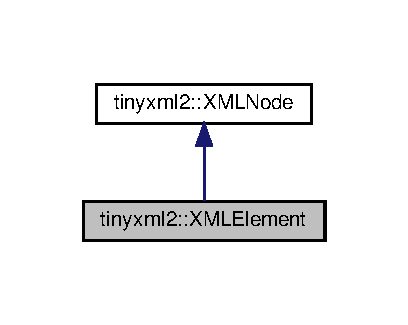
\includegraphics[width=196pt]{classtinyxml2_1_1_x_m_l_element__inherit__graph}
\end{center}
\end{figure}


Collaboration diagram for tinyxml2\+:\+:X\+M\+L\+Element\+:
\nopagebreak
\begin{figure}[H]
\begin{center}
\leavevmode
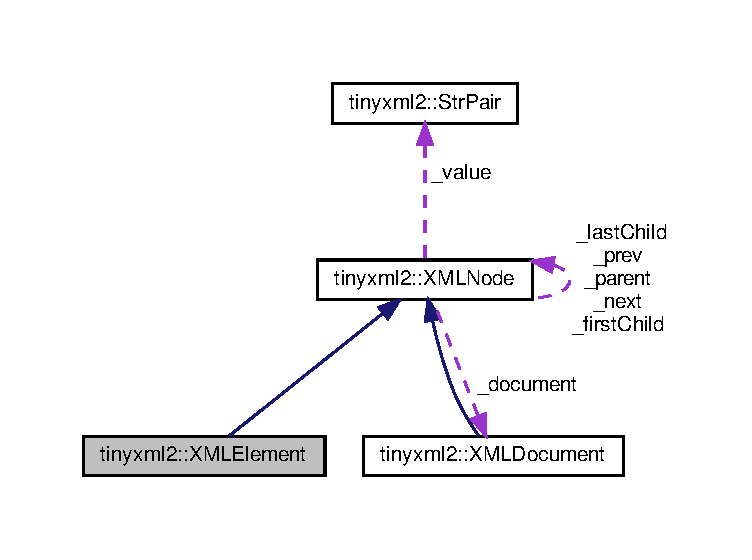
\includegraphics[width=350pt]{classtinyxml2_1_1_x_m_l_element__coll__graph}
\end{center}
\end{figure}
\subsection*{Public Types}
\begin{DoxyCompactItemize}
\item 
\mbox{\Hypertarget{classtinyxml2_1_1_x_m_l_element_ab5f90e2493c35702175235127e2935b4}\label{classtinyxml2_1_1_x_m_l_element_ab5f90e2493c35702175235127e2935b4}} 
enum {\bfseries Element\+Closing\+Type} \{ {\bfseries O\+P\+EN}, 
{\bfseries C\+L\+O\+S\+ED}, 
{\bfseries C\+L\+O\+S\+I\+NG}
 \}
\end{DoxyCompactItemize}
\subsection*{Public Member Functions}
\begin{DoxyCompactItemize}
\item 
\mbox{\Hypertarget{classtinyxml2_1_1_x_m_l_element_a63e057fb5baee1dd29f323cb85907b35}\label{classtinyxml2_1_1_x_m_l_element_a63e057fb5baee1dd29f323cb85907b35}} 
const char $\ast$ \hyperlink{classtinyxml2_1_1_x_m_l_element_a63e057fb5baee1dd29f323cb85907b35}{Name} () const
\begin{DoxyCompactList}\small\item\em Get the name of an element (which is the \hyperlink{classtinyxml2_1_1_x_m_l_node_a0485e51c670e741884cfd8362274d680}{Value()} of the node.) \end{DoxyCompactList}\item 
\mbox{\Hypertarget{classtinyxml2_1_1_x_m_l_element_a97712009a530d8cb8a63bf705f02b4f1}\label{classtinyxml2_1_1_x_m_l_element_a97712009a530d8cb8a63bf705f02b4f1}} 
void \hyperlink{classtinyxml2_1_1_x_m_l_element_a97712009a530d8cb8a63bf705f02b4f1}{Set\+Name} (const char $\ast$str, bool static\+Mem=false)
\begin{DoxyCompactList}\small\item\em Set the name of the element. \end{DoxyCompactList}\item 
\mbox{\Hypertarget{classtinyxml2_1_1_x_m_l_element_ad9ff5c2dbc15df36cf664ce1b0ea0a5d}\label{classtinyxml2_1_1_x_m_l_element_ad9ff5c2dbc15df36cf664ce1b0ea0a5d}} 
virtual \hyperlink{classtinyxml2_1_1_x_m_l_element}{X\+M\+L\+Element} $\ast$ \hyperlink{classtinyxml2_1_1_x_m_l_element_ad9ff5c2dbc15df36cf664ce1b0ea0a5d}{To\+Element} ()
\begin{DoxyCompactList}\small\item\em Safely cast to an Element, or null. \end{DoxyCompactList}\item 
\mbox{\Hypertarget{classtinyxml2_1_1_x_m_l_element_afeb353047ab8532191709dcaef07337e}\label{classtinyxml2_1_1_x_m_l_element_afeb353047ab8532191709dcaef07337e}} 
virtual const \hyperlink{classtinyxml2_1_1_x_m_l_element}{X\+M\+L\+Element} $\ast$ {\bfseries To\+Element} () const
\item 
virtual bool \hyperlink{classtinyxml2_1_1_x_m_l_element_a9b2119831e8b85827d5d3e5076788e4a}{Accept} (\hyperlink{classtinyxml2_1_1_x_m_l_visitor}{X\+M\+L\+Visitor} $\ast$visitor) const
\item 
const char $\ast$ \hyperlink{classtinyxml2_1_1_x_m_l_element_a48cf4a315cfbac7d74cd0d5ff2c5df51}{Attribute} (const char $\ast$name, const char $\ast$value=0) const
\item 
int \hyperlink{classtinyxml2_1_1_x_m_l_element_a95a89b13bb14a2d4655e2b5b406c00d4}{Int\+Attribute} (const char $\ast$name, int default\+Value=0) const
\item 
\mbox{\Hypertarget{classtinyxml2_1_1_x_m_l_element_afea43a1d4aa33e3703ddee5fc9adc26c}\label{classtinyxml2_1_1_x_m_l_element_afea43a1d4aa33e3703ddee5fc9adc26c}} 
unsigned \hyperlink{classtinyxml2_1_1_x_m_l_element_afea43a1d4aa33e3703ddee5fc9adc26c}{Unsigned\+Attribute} (const char $\ast$name, unsigned default\+Value=0) const
\begin{DoxyCompactList}\small\item\em See \hyperlink{classtinyxml2_1_1_x_m_l_element_a95a89b13bb14a2d4655e2b5b406c00d4}{Int\+Attribute()} \end{DoxyCompactList}\item 
\mbox{\Hypertarget{classtinyxml2_1_1_x_m_l_element_a66d96972adecd816194191f13cc4a0a0}\label{classtinyxml2_1_1_x_m_l_element_a66d96972adecd816194191f13cc4a0a0}} 
int64\+\_\+t \hyperlink{classtinyxml2_1_1_x_m_l_element_a66d96972adecd816194191f13cc4a0a0}{Int64\+Attribute} (const char $\ast$name, int64\+\_\+t default\+Value=0) const
\begin{DoxyCompactList}\small\item\em See \hyperlink{classtinyxml2_1_1_x_m_l_element_a95a89b13bb14a2d4655e2b5b406c00d4}{Int\+Attribute()} \end{DoxyCompactList}\item 
\mbox{\Hypertarget{classtinyxml2_1_1_x_m_l_element_a226502bab8f1be7ede1fdd255398eb85}\label{classtinyxml2_1_1_x_m_l_element_a226502bab8f1be7ede1fdd255398eb85}} 
uint64\+\_\+t \hyperlink{classtinyxml2_1_1_x_m_l_element_a226502bab8f1be7ede1fdd255398eb85}{Unsigned64\+Attribute} (const char $\ast$name, uint64\+\_\+t default\+Value=0) const
\begin{DoxyCompactList}\small\item\em See \hyperlink{classtinyxml2_1_1_x_m_l_element_a95a89b13bb14a2d4655e2b5b406c00d4}{Int\+Attribute()} \end{DoxyCompactList}\item 
\mbox{\Hypertarget{classtinyxml2_1_1_x_m_l_element_a53eda26131e1ad1031ef8ec8adb51bd8}\label{classtinyxml2_1_1_x_m_l_element_a53eda26131e1ad1031ef8ec8adb51bd8}} 
bool \hyperlink{classtinyxml2_1_1_x_m_l_element_a53eda26131e1ad1031ef8ec8adb51bd8}{Bool\+Attribute} (const char $\ast$name, bool default\+Value=false) const
\begin{DoxyCompactList}\small\item\em See \hyperlink{classtinyxml2_1_1_x_m_l_element_a95a89b13bb14a2d4655e2b5b406c00d4}{Int\+Attribute()} \end{DoxyCompactList}\item 
\mbox{\Hypertarget{classtinyxml2_1_1_x_m_l_element_a10a90c505aea716bf073eea1c97f33b5}\label{classtinyxml2_1_1_x_m_l_element_a10a90c505aea716bf073eea1c97f33b5}} 
double \hyperlink{classtinyxml2_1_1_x_m_l_element_a10a90c505aea716bf073eea1c97f33b5}{Double\+Attribute} (const char $\ast$name, double default\+Value=0) const
\begin{DoxyCompactList}\small\item\em See \hyperlink{classtinyxml2_1_1_x_m_l_element_a95a89b13bb14a2d4655e2b5b406c00d4}{Int\+Attribute()} \end{DoxyCompactList}\item 
\mbox{\Hypertarget{classtinyxml2_1_1_x_m_l_element_ab1f4be2332e27dc640e9b6abd01d64dd}\label{classtinyxml2_1_1_x_m_l_element_ab1f4be2332e27dc640e9b6abd01d64dd}} 
float \hyperlink{classtinyxml2_1_1_x_m_l_element_ab1f4be2332e27dc640e9b6abd01d64dd}{Float\+Attribute} (const char $\ast$name, float default\+Value=0) const
\begin{DoxyCompactList}\small\item\em See \hyperlink{classtinyxml2_1_1_x_m_l_element_a95a89b13bb14a2d4655e2b5b406c00d4}{Int\+Attribute()} \end{DoxyCompactList}\item 
X\+M\+L\+Error \hyperlink{classtinyxml2_1_1_x_m_l_element_a8a78bc1187c1c45ad89f2690eab567b1}{Query\+Int\+Attribute} (const char $\ast$name, int $\ast$value) const
\item 
\mbox{\Hypertarget{classtinyxml2_1_1_x_m_l_element_a26fc84cbfba6769dafcfbf256c05e22f}\label{classtinyxml2_1_1_x_m_l_element_a26fc84cbfba6769dafcfbf256c05e22f}} 
X\+M\+L\+Error \hyperlink{classtinyxml2_1_1_x_m_l_element_a26fc84cbfba6769dafcfbf256c05e22f}{Query\+Unsigned\+Attribute} (const char $\ast$name, unsigned int $\ast$value) const
\begin{DoxyCompactList}\small\item\em See \hyperlink{classtinyxml2_1_1_x_m_l_element_a8a78bc1187c1c45ad89f2690eab567b1}{Query\+Int\+Attribute()} \end{DoxyCompactList}\item 
\mbox{\Hypertarget{classtinyxml2_1_1_x_m_l_element_a7c0955d80b6f8d196744eacb0f6e90a8}\label{classtinyxml2_1_1_x_m_l_element_a7c0955d80b6f8d196744eacb0f6e90a8}} 
X\+M\+L\+Error \hyperlink{classtinyxml2_1_1_x_m_l_element_a7c0955d80b6f8d196744eacb0f6e90a8}{Query\+Int64\+Attribute} (const char $\ast$name, int64\+\_\+t $\ast$value) const
\begin{DoxyCompactList}\small\item\em See \hyperlink{classtinyxml2_1_1_x_m_l_element_a8a78bc1187c1c45ad89f2690eab567b1}{Query\+Int\+Attribute()} \end{DoxyCompactList}\item 
\mbox{\Hypertarget{classtinyxml2_1_1_x_m_l_element_a13dd590b5d3958ce2ed79844aacd9405}\label{classtinyxml2_1_1_x_m_l_element_a13dd590b5d3958ce2ed79844aacd9405}} 
X\+M\+L\+Error \hyperlink{classtinyxml2_1_1_x_m_l_element_a13dd590b5d3958ce2ed79844aacd9405}{Query\+Unsigned64\+Attribute} (const char $\ast$name, uint64\+\_\+t $\ast$value) const
\begin{DoxyCompactList}\small\item\em See \hyperlink{classtinyxml2_1_1_x_m_l_element_a8a78bc1187c1c45ad89f2690eab567b1}{Query\+Int\+Attribute()} \end{DoxyCompactList}\item 
\mbox{\Hypertarget{classtinyxml2_1_1_x_m_l_element_a14c1bb77c39689838be01838d86ca872}\label{classtinyxml2_1_1_x_m_l_element_a14c1bb77c39689838be01838d86ca872}} 
X\+M\+L\+Error \hyperlink{classtinyxml2_1_1_x_m_l_element_a14c1bb77c39689838be01838d86ca872}{Query\+Bool\+Attribute} (const char $\ast$name, bool $\ast$value) const
\begin{DoxyCompactList}\small\item\em See \hyperlink{classtinyxml2_1_1_x_m_l_element_a8a78bc1187c1c45ad89f2690eab567b1}{Query\+Int\+Attribute()} \end{DoxyCompactList}\item 
\mbox{\Hypertarget{classtinyxml2_1_1_x_m_l_element_a5f0964e2dbd8e2ee7fce9beab689443c}\label{classtinyxml2_1_1_x_m_l_element_a5f0964e2dbd8e2ee7fce9beab689443c}} 
X\+M\+L\+Error \hyperlink{classtinyxml2_1_1_x_m_l_element_a5f0964e2dbd8e2ee7fce9beab689443c}{Query\+Double\+Attribute} (const char $\ast$name, double $\ast$value) const
\begin{DoxyCompactList}\small\item\em See \hyperlink{classtinyxml2_1_1_x_m_l_element_a8a78bc1187c1c45ad89f2690eab567b1}{Query\+Int\+Attribute()} \end{DoxyCompactList}\item 
\mbox{\Hypertarget{classtinyxml2_1_1_x_m_l_element_acd5eeddf6002ef90806af794b9d9a5a5}\label{classtinyxml2_1_1_x_m_l_element_acd5eeddf6002ef90806af794b9d9a5a5}} 
X\+M\+L\+Error \hyperlink{classtinyxml2_1_1_x_m_l_element_acd5eeddf6002ef90806af794b9d9a5a5}{Query\+Float\+Attribute} (const char $\ast$name, float $\ast$value) const
\begin{DoxyCompactList}\small\item\em See \hyperlink{classtinyxml2_1_1_x_m_l_element_a8a78bc1187c1c45ad89f2690eab567b1}{Query\+Int\+Attribute()} \end{DoxyCompactList}\item 
\mbox{\Hypertarget{classtinyxml2_1_1_x_m_l_element_adb8ae765f98d0c5037faec48deea78bc}\label{classtinyxml2_1_1_x_m_l_element_adb8ae765f98d0c5037faec48deea78bc}} 
X\+M\+L\+Error \hyperlink{classtinyxml2_1_1_x_m_l_element_adb8ae765f98d0c5037faec48deea78bc}{Query\+String\+Attribute} (const char $\ast$name, const char $\ast$$\ast$value) const
\begin{DoxyCompactList}\small\item\em See \hyperlink{classtinyxml2_1_1_x_m_l_element_a8a78bc1187c1c45ad89f2690eab567b1}{Query\+Int\+Attribute()} \end{DoxyCompactList}\item 
X\+M\+L\+Error \hyperlink{classtinyxml2_1_1_x_m_l_element_a5b7df3bed2b8954eabf227fa204522eb}{Query\+Attribute} (const char $\ast$name, int $\ast$value) const
\item 
\mbox{\Hypertarget{classtinyxml2_1_1_x_m_l_element_a432276ea6e034cad19ad66de887ee13c}\label{classtinyxml2_1_1_x_m_l_element_a432276ea6e034cad19ad66de887ee13c}} 
X\+M\+L\+Error {\bfseries Query\+Attribute} (const char $\ast$name, unsigned int $\ast$value) const
\item 
\mbox{\Hypertarget{classtinyxml2_1_1_x_m_l_element_a4867aea7a812acf7f00a915e4eaeaf3e}\label{classtinyxml2_1_1_x_m_l_element_a4867aea7a812acf7f00a915e4eaeaf3e}} 
X\+M\+L\+Error {\bfseries Query\+Attribute} (const char $\ast$name, int64\+\_\+t $\ast$value) const
\item 
\mbox{\Hypertarget{classtinyxml2_1_1_x_m_l_element_ad2175dd6a927f7b0c5bfcde727da2b35}\label{classtinyxml2_1_1_x_m_l_element_ad2175dd6a927f7b0c5bfcde727da2b35}} 
X\+M\+L\+Error {\bfseries Query\+Attribute} (const char $\ast$name, uint64\+\_\+t $\ast$value) const
\item 
\mbox{\Hypertarget{classtinyxml2_1_1_x_m_l_element_a17139a22f2552439a7c2780e8e901522}\label{classtinyxml2_1_1_x_m_l_element_a17139a22f2552439a7c2780e8e901522}} 
X\+M\+L\+Error {\bfseries Query\+Attribute} (const char $\ast$name, bool $\ast$value) const
\item 
\mbox{\Hypertarget{classtinyxml2_1_1_x_m_l_element_a4f4da49900e82e25d163a7c0325fcc5f}\label{classtinyxml2_1_1_x_m_l_element_a4f4da49900e82e25d163a7c0325fcc5f}} 
X\+M\+L\+Error {\bfseries Query\+Attribute} (const char $\ast$name, double $\ast$value) const
\item 
\mbox{\Hypertarget{classtinyxml2_1_1_x_m_l_element_ac85b18ccd9ee8a79a2fd97cc593aae43}\label{classtinyxml2_1_1_x_m_l_element_ac85b18ccd9ee8a79a2fd97cc593aae43}} 
X\+M\+L\+Error {\bfseries Query\+Attribute} (const char $\ast$name, float $\ast$value) const
\item 
\mbox{\Hypertarget{classtinyxml2_1_1_x_m_l_element_a11943abf2d0831548c3790dd5d9f119c}\label{classtinyxml2_1_1_x_m_l_element_a11943abf2d0831548c3790dd5d9f119c}} 
void \hyperlink{classtinyxml2_1_1_x_m_l_element_a11943abf2d0831548c3790dd5d9f119c}{Set\+Attribute} (const char $\ast$name, const char $\ast$value)
\begin{DoxyCompactList}\small\item\em Sets the named attribute to value. \end{DoxyCompactList}\item 
\mbox{\Hypertarget{classtinyxml2_1_1_x_m_l_element_aae6568c64c7f1cc88be8461ba41a79cf}\label{classtinyxml2_1_1_x_m_l_element_aae6568c64c7f1cc88be8461ba41a79cf}} 
void \hyperlink{classtinyxml2_1_1_x_m_l_element_aae6568c64c7f1cc88be8461ba41a79cf}{Set\+Attribute} (const char $\ast$name, int value)
\begin{DoxyCompactList}\small\item\em Sets the named attribute to value. \end{DoxyCompactList}\item 
\mbox{\Hypertarget{classtinyxml2_1_1_x_m_l_element_ae143997e90064ba82326b29a9930ea8f}\label{classtinyxml2_1_1_x_m_l_element_ae143997e90064ba82326b29a9930ea8f}} 
void \hyperlink{classtinyxml2_1_1_x_m_l_element_ae143997e90064ba82326b29a9930ea8f}{Set\+Attribute} (const char $\ast$name, unsigned value)
\begin{DoxyCompactList}\small\item\em Sets the named attribute to value. \end{DoxyCompactList}\item 
\mbox{\Hypertarget{classtinyxml2_1_1_x_m_l_element_aaeefdf9171fec91b13a776b42299b0dd}\label{classtinyxml2_1_1_x_m_l_element_aaeefdf9171fec91b13a776b42299b0dd}} 
void \hyperlink{classtinyxml2_1_1_x_m_l_element_aaeefdf9171fec91b13a776b42299b0dd}{Set\+Attribute} (const char $\ast$name, int64\+\_\+t value)
\begin{DoxyCompactList}\small\item\em Sets the named attribute to value. \end{DoxyCompactList}\item 
\mbox{\Hypertarget{classtinyxml2_1_1_x_m_l_element_ad598868c0599ddc4695dab18552c308d}\label{classtinyxml2_1_1_x_m_l_element_ad598868c0599ddc4695dab18552c308d}} 
void \hyperlink{classtinyxml2_1_1_x_m_l_element_ad598868c0599ddc4695dab18552c308d}{Set\+Attribute} (const char $\ast$name, uint64\+\_\+t value)
\begin{DoxyCompactList}\small\item\em Sets the named attribute to value. \end{DoxyCompactList}\item 
\mbox{\Hypertarget{classtinyxml2_1_1_x_m_l_element_aa848b696e6a75e4e545c6da9893b11e1}\label{classtinyxml2_1_1_x_m_l_element_aa848b696e6a75e4e545c6da9893b11e1}} 
void \hyperlink{classtinyxml2_1_1_x_m_l_element_aa848b696e6a75e4e545c6da9893b11e1}{Set\+Attribute} (const char $\ast$name, bool value)
\begin{DoxyCompactList}\small\item\em Sets the named attribute to value. \end{DoxyCompactList}\item 
\mbox{\Hypertarget{classtinyxml2_1_1_x_m_l_element_a233397ee81e70eb5d4b814c5f8698533}\label{classtinyxml2_1_1_x_m_l_element_a233397ee81e70eb5d4b814c5f8698533}} 
void \hyperlink{classtinyxml2_1_1_x_m_l_element_a233397ee81e70eb5d4b814c5f8698533}{Set\+Attribute} (const char $\ast$name, double value)
\begin{DoxyCompactList}\small\item\em Sets the named attribute to value. \end{DoxyCompactList}\item 
\mbox{\Hypertarget{classtinyxml2_1_1_x_m_l_element_a554b70d882e65b28fc084b23df9b9759}\label{classtinyxml2_1_1_x_m_l_element_a554b70d882e65b28fc084b23df9b9759}} 
void \hyperlink{classtinyxml2_1_1_x_m_l_element_a554b70d882e65b28fc084b23df9b9759}{Set\+Attribute} (const char $\ast$name, float value)
\begin{DoxyCompactList}\small\item\em Sets the named attribute to value. \end{DoxyCompactList}\item 
void \hyperlink{classtinyxml2_1_1_x_m_l_element_aebd45aa7118964c30b32fe12e944628a}{Delete\+Attribute} (const char $\ast$name)
\item 
\mbox{\Hypertarget{classtinyxml2_1_1_x_m_l_element_a3e191704c8d499906ec11fe2f60c6686}\label{classtinyxml2_1_1_x_m_l_element_a3e191704c8d499906ec11fe2f60c6686}} 
const \hyperlink{classtinyxml2_1_1_x_m_l_attribute}{X\+M\+L\+Attribute} $\ast$ \hyperlink{classtinyxml2_1_1_x_m_l_element_a3e191704c8d499906ec11fe2f60c6686}{First\+Attribute} () const
\begin{DoxyCompactList}\small\item\em Return the first attribute in the list. \end{DoxyCompactList}\item 
\mbox{\Hypertarget{classtinyxml2_1_1_x_m_l_element_a157750dac8037a316fd1af1a973dfa2c}\label{classtinyxml2_1_1_x_m_l_element_a157750dac8037a316fd1af1a973dfa2c}} 
const \hyperlink{classtinyxml2_1_1_x_m_l_attribute}{X\+M\+L\+Attribute} $\ast$ \hyperlink{classtinyxml2_1_1_x_m_l_element_a157750dac8037a316fd1af1a973dfa2c}{Find\+Attribute} (const char $\ast$name) const
\begin{DoxyCompactList}\small\item\em Query a specific attribute in the list. \end{DoxyCompactList}\item 
const char $\ast$ \hyperlink{classtinyxml2_1_1_x_m_l_element_a0fa5bea0a4daf3ddd503dcabb823eba6}{Get\+Text} () const
\item 
void \hyperlink{classtinyxml2_1_1_x_m_l_element_a1f9c2cd61b72af5ae708d37b7ad283ce}{Set\+Text} (const char $\ast$in\+Text)
\item 
\mbox{\Hypertarget{classtinyxml2_1_1_x_m_l_element_aeae8917b5ea6060b3c08d4e3d8d632d7}\label{classtinyxml2_1_1_x_m_l_element_aeae8917b5ea6060b3c08d4e3d8d632d7}} 
void \hyperlink{classtinyxml2_1_1_x_m_l_element_aeae8917b5ea6060b3c08d4e3d8d632d7}{Set\+Text} (int value)
\begin{DoxyCompactList}\small\item\em Convenience method for setting text inside an element. See \hyperlink{classtinyxml2_1_1_x_m_l_element_a1f9c2cd61b72af5ae708d37b7ad283ce}{Set\+Text()} for important limitations. \end{DoxyCompactList}\item 
\mbox{\Hypertarget{classtinyxml2_1_1_x_m_l_element_a7bbfcc11d516598bc924a8fba4d08597}\label{classtinyxml2_1_1_x_m_l_element_a7bbfcc11d516598bc924a8fba4d08597}} 
void \hyperlink{classtinyxml2_1_1_x_m_l_element_a7bbfcc11d516598bc924a8fba4d08597}{Set\+Text} (unsigned value)
\begin{DoxyCompactList}\small\item\em Convenience method for setting text inside an element. See \hyperlink{classtinyxml2_1_1_x_m_l_element_a1f9c2cd61b72af5ae708d37b7ad283ce}{Set\+Text()} for important limitations. \end{DoxyCompactList}\item 
\mbox{\Hypertarget{classtinyxml2_1_1_x_m_l_element_a7b62cd33acdfeff7ea2b1b330d4368e4}\label{classtinyxml2_1_1_x_m_l_element_a7b62cd33acdfeff7ea2b1b330d4368e4}} 
void \hyperlink{classtinyxml2_1_1_x_m_l_element_a7b62cd33acdfeff7ea2b1b330d4368e4}{Set\+Text} (int64\+\_\+t value)
\begin{DoxyCompactList}\small\item\em Convenience method for setting text inside an element. See \hyperlink{classtinyxml2_1_1_x_m_l_element_a1f9c2cd61b72af5ae708d37b7ad283ce}{Set\+Text()} for important limitations. \end{DoxyCompactList}\item 
\mbox{\Hypertarget{classtinyxml2_1_1_x_m_l_element_a6e615bc745afd1ca8ded56d7aac02657}\label{classtinyxml2_1_1_x_m_l_element_a6e615bc745afd1ca8ded56d7aac02657}} 
void \hyperlink{classtinyxml2_1_1_x_m_l_element_a6e615bc745afd1ca8ded56d7aac02657}{Set\+Text} (uint64\+\_\+t value)
\begin{DoxyCompactList}\small\item\em Convenience method for setting text inside an element. See \hyperlink{classtinyxml2_1_1_x_m_l_element_a1f9c2cd61b72af5ae708d37b7ad283ce}{Set\+Text()} for important limitations. \end{DoxyCompactList}\item 
\mbox{\Hypertarget{classtinyxml2_1_1_x_m_l_element_ae4b543d6770de76fb6ab68e541c192a4}\label{classtinyxml2_1_1_x_m_l_element_ae4b543d6770de76fb6ab68e541c192a4}} 
void \hyperlink{classtinyxml2_1_1_x_m_l_element_ae4b543d6770de76fb6ab68e541c192a4}{Set\+Text} (bool value)
\begin{DoxyCompactList}\small\item\em Convenience method for setting text inside an element. See \hyperlink{classtinyxml2_1_1_x_m_l_element_a1f9c2cd61b72af5ae708d37b7ad283ce}{Set\+Text()} for important limitations. \end{DoxyCompactList}\item 
\mbox{\Hypertarget{classtinyxml2_1_1_x_m_l_element_a67bd77ac9aaeff58ff20b4275a65ba4e}\label{classtinyxml2_1_1_x_m_l_element_a67bd77ac9aaeff58ff20b4275a65ba4e}} 
void \hyperlink{classtinyxml2_1_1_x_m_l_element_a67bd77ac9aaeff58ff20b4275a65ba4e}{Set\+Text} (double value)
\begin{DoxyCompactList}\small\item\em Convenience method for setting text inside an element. See \hyperlink{classtinyxml2_1_1_x_m_l_element_a1f9c2cd61b72af5ae708d37b7ad283ce}{Set\+Text()} for important limitations. \end{DoxyCompactList}\item 
\mbox{\Hypertarget{classtinyxml2_1_1_x_m_l_element_a51d560da5ae3ad6b75e0ab9ffb2ae42a}\label{classtinyxml2_1_1_x_m_l_element_a51d560da5ae3ad6b75e0ab9ffb2ae42a}} 
void \hyperlink{classtinyxml2_1_1_x_m_l_element_a51d560da5ae3ad6b75e0ab9ffb2ae42a}{Set\+Text} (float value)
\begin{DoxyCompactList}\small\item\em Convenience method for setting text inside an element. See \hyperlink{classtinyxml2_1_1_x_m_l_element_a1f9c2cd61b72af5ae708d37b7ad283ce}{Set\+Text()} for important limitations. \end{DoxyCompactList}\item 
X\+M\+L\+Error \hyperlink{classtinyxml2_1_1_x_m_l_element_a926357996bef633cb736e1a558419632}{Query\+Int\+Text} (int $\ast$ival) const
\item 
\mbox{\Hypertarget{classtinyxml2_1_1_x_m_l_element_a14d38aa4b5e18a46274a27425188a6a1}\label{classtinyxml2_1_1_x_m_l_element_a14d38aa4b5e18a46274a27425188a6a1}} 
X\+M\+L\+Error \hyperlink{classtinyxml2_1_1_x_m_l_element_a14d38aa4b5e18a46274a27425188a6a1}{Query\+Unsigned\+Text} (unsigned $\ast$uval) const
\begin{DoxyCompactList}\small\item\em See \hyperlink{classtinyxml2_1_1_x_m_l_element_a926357996bef633cb736e1a558419632}{Query\+Int\+Text()} \end{DoxyCompactList}\item 
\mbox{\Hypertarget{classtinyxml2_1_1_x_m_l_element_a120c538c8eead169e635dbc70fb226d8}\label{classtinyxml2_1_1_x_m_l_element_a120c538c8eead169e635dbc70fb226d8}} 
X\+M\+L\+Error \hyperlink{classtinyxml2_1_1_x_m_l_element_a120c538c8eead169e635dbc70fb226d8}{Query\+Int64\+Text} (int64\+\_\+t $\ast$uval) const
\begin{DoxyCompactList}\small\item\em See \hyperlink{classtinyxml2_1_1_x_m_l_element_a926357996bef633cb736e1a558419632}{Query\+Int\+Text()} \end{DoxyCompactList}\item 
\mbox{\Hypertarget{classtinyxml2_1_1_x_m_l_element_ac2239b3bd172ad8f5b78d04d4236144b}\label{classtinyxml2_1_1_x_m_l_element_ac2239b3bd172ad8f5b78d04d4236144b}} 
X\+M\+L\+Error \hyperlink{classtinyxml2_1_1_x_m_l_element_ac2239b3bd172ad8f5b78d04d4236144b}{Query\+Unsigned64\+Text} (uint64\+\_\+t $\ast$uval) const
\begin{DoxyCompactList}\small\item\em See \hyperlink{classtinyxml2_1_1_x_m_l_element_a926357996bef633cb736e1a558419632}{Query\+Int\+Text()} \end{DoxyCompactList}\item 
\mbox{\Hypertarget{classtinyxml2_1_1_x_m_l_element_a3fe5417d59eb8f5c4afe924b7d332736}\label{classtinyxml2_1_1_x_m_l_element_a3fe5417d59eb8f5c4afe924b7d332736}} 
X\+M\+L\+Error \hyperlink{classtinyxml2_1_1_x_m_l_element_a3fe5417d59eb8f5c4afe924b7d332736}{Query\+Bool\+Text} (bool $\ast$bval) const
\begin{DoxyCompactList}\small\item\em See \hyperlink{classtinyxml2_1_1_x_m_l_element_a926357996bef633cb736e1a558419632}{Query\+Int\+Text()} \end{DoxyCompactList}\item 
\mbox{\Hypertarget{classtinyxml2_1_1_x_m_l_element_a684679c99bb036a25652744cec6c4d96}\label{classtinyxml2_1_1_x_m_l_element_a684679c99bb036a25652744cec6c4d96}} 
X\+M\+L\+Error \hyperlink{classtinyxml2_1_1_x_m_l_element_a684679c99bb036a25652744cec6c4d96}{Query\+Double\+Text} (double $\ast$dval) const
\begin{DoxyCompactList}\small\item\em See \hyperlink{classtinyxml2_1_1_x_m_l_element_a926357996bef633cb736e1a558419632}{Query\+Int\+Text()} \end{DoxyCompactList}\item 
\mbox{\Hypertarget{classtinyxml2_1_1_x_m_l_element_afa332afedd93210daa6d44b88eb11e29}\label{classtinyxml2_1_1_x_m_l_element_afa332afedd93210daa6d44b88eb11e29}} 
X\+M\+L\+Error \hyperlink{classtinyxml2_1_1_x_m_l_element_afa332afedd93210daa6d44b88eb11e29}{Query\+Float\+Text} (float $\ast$fval) const
\begin{DoxyCompactList}\small\item\em See \hyperlink{classtinyxml2_1_1_x_m_l_element_a926357996bef633cb736e1a558419632}{Query\+Int\+Text()} \end{DoxyCompactList}\item 
\mbox{\Hypertarget{classtinyxml2_1_1_x_m_l_element_a37b0636adebb8a1a1bc965f60824cb3e}\label{classtinyxml2_1_1_x_m_l_element_a37b0636adebb8a1a1bc965f60824cb3e}} 
int {\bfseries Int\+Text} (int default\+Value=0) const
\item 
\mbox{\Hypertarget{classtinyxml2_1_1_x_m_l_element_a49bad014ffcc17b0b6119d5b2c97dfb5}\label{classtinyxml2_1_1_x_m_l_element_a49bad014ffcc17b0b6119d5b2c97dfb5}} 
unsigned \hyperlink{classtinyxml2_1_1_x_m_l_element_a49bad014ffcc17b0b6119d5b2c97dfb5}{Unsigned\+Text} (unsigned default\+Value=0) const
\begin{DoxyCompactList}\small\item\em See \hyperlink{classtinyxml2_1_1_x_m_l_element_a926357996bef633cb736e1a558419632}{Query\+Int\+Text()} \end{DoxyCompactList}\item 
\mbox{\Hypertarget{classtinyxml2_1_1_x_m_l_element_aab6151f7e3b4c2c0a8234e262d7b6b8a}\label{classtinyxml2_1_1_x_m_l_element_aab6151f7e3b4c2c0a8234e262d7b6b8a}} 
int64\+\_\+t \hyperlink{classtinyxml2_1_1_x_m_l_element_aab6151f7e3b4c2c0a8234e262d7b6b8a}{Int64\+Text} (int64\+\_\+t default\+Value=0) const
\begin{DoxyCompactList}\small\item\em See \hyperlink{classtinyxml2_1_1_x_m_l_element_a926357996bef633cb736e1a558419632}{Query\+Int\+Text()} \end{DoxyCompactList}\item 
\mbox{\Hypertarget{classtinyxml2_1_1_x_m_l_element_af48c1023abbac1acdf4927c51c3a5f0c}\label{classtinyxml2_1_1_x_m_l_element_af48c1023abbac1acdf4927c51c3a5f0c}} 
uint64\+\_\+t \hyperlink{classtinyxml2_1_1_x_m_l_element_af48c1023abbac1acdf4927c51c3a5f0c}{Unsigned64\+Text} (uint64\+\_\+t default\+Value=0) const
\begin{DoxyCompactList}\small\item\em See \hyperlink{classtinyxml2_1_1_x_m_l_element_a926357996bef633cb736e1a558419632}{Query\+Int\+Text()} \end{DoxyCompactList}\item 
\mbox{\Hypertarget{classtinyxml2_1_1_x_m_l_element_a68569f59f6382bcea7f5013ec59736d2}\label{classtinyxml2_1_1_x_m_l_element_a68569f59f6382bcea7f5013ec59736d2}} 
bool \hyperlink{classtinyxml2_1_1_x_m_l_element_a68569f59f6382bcea7f5013ec59736d2}{Bool\+Text} (bool default\+Value=false) const
\begin{DoxyCompactList}\small\item\em See \hyperlink{classtinyxml2_1_1_x_m_l_element_a926357996bef633cb736e1a558419632}{Query\+Int\+Text()} \end{DoxyCompactList}\item 
\mbox{\Hypertarget{classtinyxml2_1_1_x_m_l_element_a81b1ff0cf2f2cd09be8badc08b39a2b7}\label{classtinyxml2_1_1_x_m_l_element_a81b1ff0cf2f2cd09be8badc08b39a2b7}} 
double \hyperlink{classtinyxml2_1_1_x_m_l_element_a81b1ff0cf2f2cd09be8badc08b39a2b7}{Double\+Text} (double default\+Value=0) const
\begin{DoxyCompactList}\small\item\em See \hyperlink{classtinyxml2_1_1_x_m_l_element_a926357996bef633cb736e1a558419632}{Query\+Int\+Text()} \end{DoxyCompactList}\item 
\mbox{\Hypertarget{classtinyxml2_1_1_x_m_l_element_a45444eb21f99ca46101545992dc2e927}\label{classtinyxml2_1_1_x_m_l_element_a45444eb21f99ca46101545992dc2e927}} 
float \hyperlink{classtinyxml2_1_1_x_m_l_element_a45444eb21f99ca46101545992dc2e927}{Float\+Text} (float default\+Value=0) const
\begin{DoxyCompactList}\small\item\em See \hyperlink{classtinyxml2_1_1_x_m_l_element_a926357996bef633cb736e1a558419632}{Query\+Int\+Text()} \end{DoxyCompactList}\item 
\mbox{\Hypertarget{classtinyxml2_1_1_x_m_l_element_a6965ff89557f27d4082d7043d5145555}\label{classtinyxml2_1_1_x_m_l_element_a6965ff89557f27d4082d7043d5145555}} 
Element\+Closing\+Type {\bfseries Closing\+Type} () const
\item 
virtual \hyperlink{classtinyxml2_1_1_x_m_l_node}{X\+M\+L\+Node} $\ast$ \hyperlink{classtinyxml2_1_1_x_m_l_element_aafa2807a45b28fe096b29d76e6a13b7c}{Shallow\+Clone} (\hyperlink{classtinyxml2_1_1_x_m_l_document}{X\+M\+L\+Document} $\ast$document) const
\item 
virtual bool \hyperlink{classtinyxml2_1_1_x_m_l_element_a61ffd7bf918a9db4aa6203d855ac5ec2}{Shallow\+Equal} (const \hyperlink{classtinyxml2_1_1_x_m_l_node}{X\+M\+L\+Node} $\ast$compare) const
\end{DoxyCompactItemize}
\subsection*{Protected Member Functions}
\begin{DoxyCompactItemize}
\item 
\mbox{\Hypertarget{classtinyxml2_1_1_x_m_l_element_a072998100b7d0ba5e8aeac6dd6dfb31b}\label{classtinyxml2_1_1_x_m_l_element_a072998100b7d0ba5e8aeac6dd6dfb31b}} 
char $\ast$ {\bfseries Parse\+Deep} (char $\ast$p, \hyperlink{classtinyxml2_1_1_str_pair}{Str\+Pair} $\ast$parent\+End\+Tag, int $\ast$cur\+Line\+Num\+Ptr)
\end{DoxyCompactItemize}
\subsection*{Friends}
\begin{DoxyCompactItemize}
\item 
\mbox{\Hypertarget{classtinyxml2_1_1_x_m_l_element_a4eee3bda60c60a30e4e8cd4ea91c4c6e}\label{classtinyxml2_1_1_x_m_l_element_a4eee3bda60c60a30e4e8cd4ea91c4c6e}} 
class {\bfseries X\+M\+L\+Document}
\end{DoxyCompactItemize}
\subsection*{Additional Inherited Members}


\subsection{Detailed Description}
The element is a container class. It has a value, the element name, and can contain other elements, text, comments, and unknowns. Elements also contain an arbitrary number of attributes. 

\subsection{Member Function Documentation}
\mbox{\Hypertarget{classtinyxml2_1_1_x_m_l_element_a9b2119831e8b85827d5d3e5076788e4a}\label{classtinyxml2_1_1_x_m_l_element_a9b2119831e8b85827d5d3e5076788e4a}} 
\index{tinyxml2\+::\+X\+M\+L\+Element@{tinyxml2\+::\+X\+M\+L\+Element}!Accept@{Accept}}
\index{Accept@{Accept}!tinyxml2\+::\+X\+M\+L\+Element@{tinyxml2\+::\+X\+M\+L\+Element}}
\subsubsection{\texorpdfstring{Accept()}{Accept()}}
{\footnotesize\ttfamily bool tinyxml2\+::\+X\+M\+L\+Element\+::\+Accept (\begin{DoxyParamCaption}\item[{\hyperlink{classtinyxml2_1_1_x_m_l_visitor}{X\+M\+L\+Visitor} $\ast$}]{visitor }\end{DoxyParamCaption}) const\hspace{0.3cm}{\ttfamily [virtual]}}

Accept a hierarchical visit of the nodes in the Tiny\+X\+M\+L-\/2 D\+OM. Every node in the X\+ML tree will be conditionally visited and the host will be called back via the \hyperlink{classtinyxml2_1_1_x_m_l_visitor}{X\+M\+L\+Visitor} interface.

This is essentially a S\+AX interface for Tiny\+X\+M\+L-\/2. (Note however it doesn\textquotesingle{}t re-\/parse the X\+ML for the callbacks, so the performance of Tiny\+X\+M\+L-\/2 is unchanged by using this interface versus any other.)

The interface has been based on ideas from\+:


\begin{DoxyItemize}
\item \href{http://www.saxproject.org/}{\tt http\+://www.\+saxproject.\+org/}
\item \href{http://c2.com/cgi/wiki?HierarchicalVisitorPattern}{\tt http\+://c2.\+com/cgi/wiki?\+Hierarchical\+Visitor\+Pattern}
\end{DoxyItemize}

Which are both good references for \char`\"{}visiting\char`\"{}.

An example of using \hyperlink{classtinyxml2_1_1_x_m_l_element_a9b2119831e8b85827d5d3e5076788e4a}{Accept()}\+: \begin{DoxyVerb}XMLPrinter printer;
tinyxmlDoc.Accept( &printer );
const char* xmlcstr = printer.CStr();
\end{DoxyVerb}
 

Implements \hyperlink{classtinyxml2_1_1_x_m_l_node_a81e66df0a44c67a7af17f3b77a152785}{tinyxml2\+::\+X\+M\+L\+Node}.

\mbox{\Hypertarget{classtinyxml2_1_1_x_m_l_element_a48cf4a315cfbac7d74cd0d5ff2c5df51}\label{classtinyxml2_1_1_x_m_l_element_a48cf4a315cfbac7d74cd0d5ff2c5df51}} 
\index{tinyxml2\+::\+X\+M\+L\+Element@{tinyxml2\+::\+X\+M\+L\+Element}!Attribute@{Attribute}}
\index{Attribute@{Attribute}!tinyxml2\+::\+X\+M\+L\+Element@{tinyxml2\+::\+X\+M\+L\+Element}}
\subsubsection{\texorpdfstring{Attribute()}{Attribute()}}
{\footnotesize\ttfamily const char $\ast$ tinyxml2\+::\+X\+M\+L\+Element\+::\+Attribute (\begin{DoxyParamCaption}\item[{const char $\ast$}]{name,  }\item[{const char $\ast$}]{value = {\ttfamily 0} }\end{DoxyParamCaption}) const}

Given an attribute name, \hyperlink{classtinyxml2_1_1_x_m_l_element_a48cf4a315cfbac7d74cd0d5ff2c5df51}{Attribute()} returns the value for the attribute of that name, or null if none exists. For example\+:

\begin{DoxyVerb}const char* value = ele->Attribute( "foo" );
\end{DoxyVerb}


The \textquotesingle{}value\textquotesingle{} parameter is normally null. However, if specified, the attribute will only be returned if the \textquotesingle{}name\textquotesingle{} and \textquotesingle{}value\textquotesingle{} match. This allow you to write code\+:

\begin{DoxyVerb}if ( ele->Attribute( "foo", "bar" ) ) callFooIsBar();
\end{DoxyVerb}


rather than\+: \begin{DoxyVerb}if ( ele->Attribute( "foo" ) ) {
    if ( strcmp( ele->Attribute( "foo" ), "bar" ) == 0 ) callFooIsBar();
}
\end{DoxyVerb}
 \mbox{\Hypertarget{classtinyxml2_1_1_x_m_l_element_aebd45aa7118964c30b32fe12e944628a}\label{classtinyxml2_1_1_x_m_l_element_aebd45aa7118964c30b32fe12e944628a}} 
\index{tinyxml2\+::\+X\+M\+L\+Element@{tinyxml2\+::\+X\+M\+L\+Element}!Delete\+Attribute@{Delete\+Attribute}}
\index{Delete\+Attribute@{Delete\+Attribute}!tinyxml2\+::\+X\+M\+L\+Element@{tinyxml2\+::\+X\+M\+L\+Element}}
\subsubsection{\texorpdfstring{Delete\+Attribute()}{DeleteAttribute()}}
{\footnotesize\ttfamily void tinyxml2\+::\+X\+M\+L\+Element\+::\+Delete\+Attribute (\begin{DoxyParamCaption}\item[{const char $\ast$}]{name }\end{DoxyParamCaption})}

Delete an attribute. \mbox{\Hypertarget{classtinyxml2_1_1_x_m_l_element_a0fa5bea0a4daf3ddd503dcabb823eba6}\label{classtinyxml2_1_1_x_m_l_element_a0fa5bea0a4daf3ddd503dcabb823eba6}} 
\index{tinyxml2\+::\+X\+M\+L\+Element@{tinyxml2\+::\+X\+M\+L\+Element}!Get\+Text@{Get\+Text}}
\index{Get\+Text@{Get\+Text}!tinyxml2\+::\+X\+M\+L\+Element@{tinyxml2\+::\+X\+M\+L\+Element}}
\subsubsection{\texorpdfstring{Get\+Text()}{GetText()}}
{\footnotesize\ttfamily const char $\ast$ tinyxml2\+::\+X\+M\+L\+Element\+::\+Get\+Text (\begin{DoxyParamCaption}{ }\end{DoxyParamCaption}) const}

Convenience function for easy access to the text inside an element. Although easy and concise, \hyperlink{classtinyxml2_1_1_x_m_l_element_a0fa5bea0a4daf3ddd503dcabb823eba6}{Get\+Text()} is limited compared to getting the \hyperlink{classtinyxml2_1_1_x_m_l_text}{X\+M\+L\+Text} child and accessing it directly.

If the first child of \textquotesingle{}this\textquotesingle{} is a \hyperlink{classtinyxml2_1_1_x_m_l_text}{X\+M\+L\+Text}, the \hyperlink{classtinyxml2_1_1_x_m_l_element_a0fa5bea0a4daf3ddd503dcabb823eba6}{Get\+Text()} returns the character string of the Text node, else null is returned.

This is a convenient method for getting the text of simple contained text\+: \begin{DoxyVerb}<foo>This is text</foo>
    const char* str = fooElement->GetText();
\end{DoxyVerb}


\textquotesingle{}str\textquotesingle{} will be a pointer to \char`\"{}\+This is text\char`\"{}.

Note that this function can be misleading. If the element foo was created from this X\+ML\+: \begin{DoxyVerb}    <foo><b>This is text</b></foo>
\end{DoxyVerb}


then the value of str would be null. The first child node isn\textquotesingle{}t a text node, it is another element. From this X\+ML\+: \begin{DoxyVerb}    <foo>This is <b>text</b></foo>
\end{DoxyVerb}
 \hyperlink{classtinyxml2_1_1_x_m_l_element_a0fa5bea0a4daf3ddd503dcabb823eba6}{Get\+Text()} will return \char`\"{}\+This is \char`\"{}. \mbox{\Hypertarget{classtinyxml2_1_1_x_m_l_element_a95a89b13bb14a2d4655e2b5b406c00d4}\label{classtinyxml2_1_1_x_m_l_element_a95a89b13bb14a2d4655e2b5b406c00d4}} 
\index{tinyxml2\+::\+X\+M\+L\+Element@{tinyxml2\+::\+X\+M\+L\+Element}!Int\+Attribute@{Int\+Attribute}}
\index{Int\+Attribute@{Int\+Attribute}!tinyxml2\+::\+X\+M\+L\+Element@{tinyxml2\+::\+X\+M\+L\+Element}}
\subsubsection{\texorpdfstring{Int\+Attribute()}{IntAttribute()}}
{\footnotesize\ttfamily int tinyxml2\+::\+X\+M\+L\+Element\+::\+Int\+Attribute (\begin{DoxyParamCaption}\item[{const char $\ast$}]{name,  }\item[{int}]{default\+Value = {\ttfamily 0} }\end{DoxyParamCaption}) const}

Given an attribute name, \hyperlink{classtinyxml2_1_1_x_m_l_element_a95a89b13bb14a2d4655e2b5b406c00d4}{Int\+Attribute()} returns the value of the attribute interpreted as an integer. The default value will be returned if the attribute isn\textquotesingle{}t present, or if there is an error. (For a method with error checking, see \hyperlink{classtinyxml2_1_1_x_m_l_element_a8a78bc1187c1c45ad89f2690eab567b1}{Query\+Int\+Attribute()}). \mbox{\Hypertarget{classtinyxml2_1_1_x_m_l_element_a5b7df3bed2b8954eabf227fa204522eb}\label{classtinyxml2_1_1_x_m_l_element_a5b7df3bed2b8954eabf227fa204522eb}} 
\index{tinyxml2\+::\+X\+M\+L\+Element@{tinyxml2\+::\+X\+M\+L\+Element}!Query\+Attribute@{Query\+Attribute}}
\index{Query\+Attribute@{Query\+Attribute}!tinyxml2\+::\+X\+M\+L\+Element@{tinyxml2\+::\+X\+M\+L\+Element}}
\subsubsection{\texorpdfstring{Query\+Attribute()}{QueryAttribute()}}
{\footnotesize\ttfamily X\+M\+L\+Error tinyxml2\+::\+X\+M\+L\+Element\+::\+Query\+Attribute (\begin{DoxyParamCaption}\item[{const char $\ast$}]{name,  }\item[{int $\ast$}]{value }\end{DoxyParamCaption}) const\hspace{0.3cm}{\ttfamily [inline]}}

Given an attribute name, \hyperlink{classtinyxml2_1_1_x_m_l_element_a5b7df3bed2b8954eabf227fa204522eb}{Query\+Attribute()} returns X\+M\+L\+\_\+\+S\+U\+C\+C\+E\+SS, X\+M\+L\+\_\+\+W\+R\+O\+N\+G\+\_\+\+A\+T\+T\+R\+I\+B\+U\+T\+E\+\_\+\+T\+Y\+PE if the conversion can\textquotesingle{}t be performed, or X\+M\+L\+\_\+\+N\+O\+\_\+\+A\+T\+T\+R\+I\+B\+U\+TE if the attribute doesn\textquotesingle{}t exist. It is overloaded for the primitive types, and is a generally more convenient replacement of \hyperlink{classtinyxml2_1_1_x_m_l_element_a8a78bc1187c1c45ad89f2690eab567b1}{Query\+Int\+Attribute()} and related functions.

If successful, the result of the conversion will be written to \textquotesingle{}value\textquotesingle{}. If not successful, nothing will be written to \textquotesingle{}value\textquotesingle{}. This allows you to provide default value\+:

\begin{DoxyVerb}int value = 10;
QueryAttribute( "foo", &value );        // if "foo" isn't found, value will still be 10
\end{DoxyVerb}
 \mbox{\Hypertarget{classtinyxml2_1_1_x_m_l_element_a8a78bc1187c1c45ad89f2690eab567b1}\label{classtinyxml2_1_1_x_m_l_element_a8a78bc1187c1c45ad89f2690eab567b1}} 
\index{tinyxml2\+::\+X\+M\+L\+Element@{tinyxml2\+::\+X\+M\+L\+Element}!Query\+Int\+Attribute@{Query\+Int\+Attribute}}
\index{Query\+Int\+Attribute@{Query\+Int\+Attribute}!tinyxml2\+::\+X\+M\+L\+Element@{tinyxml2\+::\+X\+M\+L\+Element}}
\subsubsection{\texorpdfstring{Query\+Int\+Attribute()}{QueryIntAttribute()}}
{\footnotesize\ttfamily X\+M\+L\+Error tinyxml2\+::\+X\+M\+L\+Element\+::\+Query\+Int\+Attribute (\begin{DoxyParamCaption}\item[{const char $\ast$}]{name,  }\item[{int $\ast$}]{value }\end{DoxyParamCaption}) const\hspace{0.3cm}{\ttfamily [inline]}}

Given an attribute name, \hyperlink{classtinyxml2_1_1_x_m_l_element_a8a78bc1187c1c45ad89f2690eab567b1}{Query\+Int\+Attribute()} returns X\+M\+L\+\_\+\+S\+U\+C\+C\+E\+SS, X\+M\+L\+\_\+\+W\+R\+O\+N\+G\+\_\+\+A\+T\+T\+R\+I\+B\+U\+T\+E\+\_\+\+T\+Y\+PE if the conversion can\textquotesingle{}t be performed, or X\+M\+L\+\_\+\+N\+O\+\_\+\+A\+T\+T\+R\+I\+B\+U\+TE if the attribute doesn\textquotesingle{}t exist. If successful, the result of the conversion will be written to \textquotesingle{}value\textquotesingle{}. If not successful, nothing will be written to \textquotesingle{}value\textquotesingle{}. This allows you to provide default value\+:

\begin{DoxyVerb}int value = 10;
QueryIntAttribute( "foo", &value );     // if "foo" isn't found, value will still be 10
\end{DoxyVerb}
 \mbox{\Hypertarget{classtinyxml2_1_1_x_m_l_element_a926357996bef633cb736e1a558419632}\label{classtinyxml2_1_1_x_m_l_element_a926357996bef633cb736e1a558419632}} 
\index{tinyxml2\+::\+X\+M\+L\+Element@{tinyxml2\+::\+X\+M\+L\+Element}!Query\+Int\+Text@{Query\+Int\+Text}}
\index{Query\+Int\+Text@{Query\+Int\+Text}!tinyxml2\+::\+X\+M\+L\+Element@{tinyxml2\+::\+X\+M\+L\+Element}}
\subsubsection{\texorpdfstring{Query\+Int\+Text()}{QueryIntText()}}
{\footnotesize\ttfamily X\+M\+L\+Error tinyxml2\+::\+X\+M\+L\+Element\+::\+Query\+Int\+Text (\begin{DoxyParamCaption}\item[{int $\ast$}]{ival }\end{DoxyParamCaption}) const}

Convenience method to query the value of a child text node. This is probably best shown by example. Given you have a document is this form\+: \begin{DoxyVerb}    <point>
        <x>1</x>
        <y>1.4</y>
    </point>
\end{DoxyVerb}


The \hyperlink{classtinyxml2_1_1_x_m_l_element_a926357996bef633cb736e1a558419632}{Query\+Int\+Text()} and similar functions provide a safe and easier way to get to the \char`\"{}value\char`\"{} of x and y.

\begin{DoxyVerb}    int x = 0;
    float y = 0;    // types of x and y are contrived for example
    const XMLElement* xElement = pointElement->FirstChildElement( "x" );
    const XMLElement* yElement = pointElement->FirstChildElement( "y" );
    xElement->QueryIntText( &x );
    yElement->QueryFloatText( &y );
\end{DoxyVerb}


\begin{DoxyReturn}{Returns}
X\+M\+L\+\_\+\+S\+U\+C\+C\+E\+SS (0) on success, X\+M\+L\+\_\+\+C\+A\+N\+\_\+\+N\+O\+T\+\_\+\+C\+O\+N\+V\+E\+R\+T\+\_\+\+T\+E\+XT if the text cannot be converted to the requested type, and X\+M\+L\+\_\+\+N\+O\+\_\+\+T\+E\+X\+T\+\_\+\+N\+O\+DE if there is no child text to query. 
\end{DoxyReturn}
\mbox{\Hypertarget{classtinyxml2_1_1_x_m_l_element_a1f9c2cd61b72af5ae708d37b7ad283ce}\label{classtinyxml2_1_1_x_m_l_element_a1f9c2cd61b72af5ae708d37b7ad283ce}} 
\index{tinyxml2\+::\+X\+M\+L\+Element@{tinyxml2\+::\+X\+M\+L\+Element}!Set\+Text@{Set\+Text}}
\index{Set\+Text@{Set\+Text}!tinyxml2\+::\+X\+M\+L\+Element@{tinyxml2\+::\+X\+M\+L\+Element}}
\subsubsection{\texorpdfstring{Set\+Text()}{SetText()}}
{\footnotesize\ttfamily void tinyxml2\+::\+X\+M\+L\+Element\+::\+Set\+Text (\begin{DoxyParamCaption}\item[{const char $\ast$}]{in\+Text }\end{DoxyParamCaption})}

Convenience function for easy access to the text inside an element. Although easy and concise, \hyperlink{classtinyxml2_1_1_x_m_l_element_a1f9c2cd61b72af5ae708d37b7ad283ce}{Set\+Text()} is limited compared to creating an \hyperlink{classtinyxml2_1_1_x_m_l_text}{X\+M\+L\+Text} child and mutating it directly.

If the first child of \textquotesingle{}this\textquotesingle{} is a \hyperlink{classtinyxml2_1_1_x_m_l_text}{X\+M\+L\+Text}, \hyperlink{classtinyxml2_1_1_x_m_l_element_a1f9c2cd61b72af5ae708d37b7ad283ce}{Set\+Text()} sets its value to the given string, otherwise it will create a first child that is an \hyperlink{classtinyxml2_1_1_x_m_l_text}{X\+M\+L\+Text}.

This is a convenient method for setting the text of simple contained text\+: \begin{DoxyVerb}<foo>This is text</foo>
    fooElement->SetText( "Hullaballoo!" );
<foo>Hullaballoo!</foo>
\end{DoxyVerb}


Note that this function can be misleading. If the element foo was created from this X\+ML\+: \begin{DoxyVerb}    <foo><b>This is text</b></foo>
\end{DoxyVerb}


then it will not change \char`\"{}\+This is text\char`\"{}, but rather prefix it with a text element\+: \begin{DoxyVerb}    <foo>Hullaballoo!<b>This is text</b></foo>
\end{DoxyVerb}


For this X\+ML\+: \begin{DoxyVerb}    <foo />
\end{DoxyVerb}
 \hyperlink{classtinyxml2_1_1_x_m_l_element_a1f9c2cd61b72af5ae708d37b7ad283ce}{Set\+Text()} will generate \begin{DoxyVerb}    <foo>Hullaballoo!</foo>
\end{DoxyVerb}
 \mbox{\Hypertarget{classtinyxml2_1_1_x_m_l_element_aafa2807a45b28fe096b29d76e6a13b7c}\label{classtinyxml2_1_1_x_m_l_element_aafa2807a45b28fe096b29d76e6a13b7c}} 
\index{tinyxml2\+::\+X\+M\+L\+Element@{tinyxml2\+::\+X\+M\+L\+Element}!Shallow\+Clone@{Shallow\+Clone}}
\index{Shallow\+Clone@{Shallow\+Clone}!tinyxml2\+::\+X\+M\+L\+Element@{tinyxml2\+::\+X\+M\+L\+Element}}
\subsubsection{\texorpdfstring{Shallow\+Clone()}{ShallowClone()}}
{\footnotesize\ttfamily \hyperlink{classtinyxml2_1_1_x_m_l_node}{X\+M\+L\+Node} $\ast$ tinyxml2\+::\+X\+M\+L\+Element\+::\+Shallow\+Clone (\begin{DoxyParamCaption}\item[{\hyperlink{classtinyxml2_1_1_x_m_l_document}{X\+M\+L\+Document} $\ast$}]{document }\end{DoxyParamCaption}) const\hspace{0.3cm}{\ttfamily [virtual]}}

Make a copy of this node, but not its children. You may pass in a Document pointer that will be the owner of the new Node. If the \textquotesingle{}document\textquotesingle{} is null, then the node returned will be allocated from the current Document. (this-\/$>$\hyperlink{classtinyxml2_1_1_x_m_l_node_af343d1ef0b45c0020e62d784d7e67a68}{Get\+Document()})

Note\+: if called on a \hyperlink{classtinyxml2_1_1_x_m_l_document}{X\+M\+L\+Document}, this will return null. 

Implements \hyperlink{classtinyxml2_1_1_x_m_l_node_a8402cbd3129d20e9e6024bbcc0531283}{tinyxml2\+::\+X\+M\+L\+Node}.

\mbox{\Hypertarget{classtinyxml2_1_1_x_m_l_element_a61ffd7bf918a9db4aa6203d855ac5ec2}\label{classtinyxml2_1_1_x_m_l_element_a61ffd7bf918a9db4aa6203d855ac5ec2}} 
\index{tinyxml2\+::\+X\+M\+L\+Element@{tinyxml2\+::\+X\+M\+L\+Element}!Shallow\+Equal@{Shallow\+Equal}}
\index{Shallow\+Equal@{Shallow\+Equal}!tinyxml2\+::\+X\+M\+L\+Element@{tinyxml2\+::\+X\+M\+L\+Element}}
\subsubsection{\texorpdfstring{Shallow\+Equal()}{ShallowEqual()}}
{\footnotesize\ttfamily bool tinyxml2\+::\+X\+M\+L\+Element\+::\+Shallow\+Equal (\begin{DoxyParamCaption}\item[{const \hyperlink{classtinyxml2_1_1_x_m_l_node}{X\+M\+L\+Node} $\ast$}]{compare }\end{DoxyParamCaption}) const\hspace{0.3cm}{\ttfamily [virtual]}}

Test if 2 nodes are the same, but don\textquotesingle{}t test children. The 2 nodes do not need to be in the same Document.

Note\+: if called on a \hyperlink{classtinyxml2_1_1_x_m_l_document}{X\+M\+L\+Document}, this will return false. 

Implements \hyperlink{classtinyxml2_1_1_x_m_l_node_a7ce18b751c3ea09eac292dca264f9226}{tinyxml2\+::\+X\+M\+L\+Node}.



The documentation for this class was generated from the following files\+:\begin{DoxyCompactItemize}
\item 
/home/ijlee/workspace/sdmt/src/tinyxml2.\+h\item 
/home/ijlee/workspace/sdmt/src/tinyxml2.\+cpp\end{DoxyCompactItemize}

\hypertarget{classtinyxml2_1_1_x_m_l_handle}{}\section{tinyxml2\+:\+:X\+M\+L\+Handle Class Reference}
\label{classtinyxml2_1_1_x_m_l_handle}\index{tinyxml2\+::\+X\+M\+L\+Handle@{tinyxml2\+::\+X\+M\+L\+Handle}}


{\ttfamily \#include $<$tinyxml2.\+h$>$}

\subsection*{Public Member Functions}
\begin{DoxyCompactItemize}
\item 
\mbox{\Hypertarget{classtinyxml2_1_1_x_m_l_handle_a9c240a35c18f053509b4b97ddccd9793}\label{classtinyxml2_1_1_x_m_l_handle_a9c240a35c18f053509b4b97ddccd9793}} 
\hyperlink{classtinyxml2_1_1_x_m_l_handle_a9c240a35c18f053509b4b97ddccd9793}{X\+M\+L\+Handle} (\hyperlink{classtinyxml2_1_1_x_m_l_node}{X\+M\+L\+Node} $\ast$node)
\begin{DoxyCompactList}\small\item\em Create a handle from any node (at any depth of the tree.) This can be a null pointer. \end{DoxyCompactList}\item 
\mbox{\Hypertarget{classtinyxml2_1_1_x_m_l_handle_aa2edbc1c0d3e3e8259bd98de7f1cf500}\label{classtinyxml2_1_1_x_m_l_handle_aa2edbc1c0d3e3e8259bd98de7f1cf500}} 
\hyperlink{classtinyxml2_1_1_x_m_l_handle_aa2edbc1c0d3e3e8259bd98de7f1cf500}{X\+M\+L\+Handle} (\hyperlink{classtinyxml2_1_1_x_m_l_node}{X\+M\+L\+Node} \&node)
\begin{DoxyCompactList}\small\item\em Create a handle from a node. \end{DoxyCompactList}\item 
\mbox{\Hypertarget{classtinyxml2_1_1_x_m_l_handle_afd8e01e6018c07347b8e6d80272466aa}\label{classtinyxml2_1_1_x_m_l_handle_afd8e01e6018c07347b8e6d80272466aa}} 
\hyperlink{classtinyxml2_1_1_x_m_l_handle_afd8e01e6018c07347b8e6d80272466aa}{X\+M\+L\+Handle} (const \hyperlink{classtinyxml2_1_1_x_m_l_handle}{X\+M\+L\+Handle} \&ref)
\begin{DoxyCompactList}\small\item\em Copy constructor. \end{DoxyCompactList}\item 
\mbox{\Hypertarget{classtinyxml2_1_1_x_m_l_handle_a75b908322bb4b83be3281b6845252b20}\label{classtinyxml2_1_1_x_m_l_handle_a75b908322bb4b83be3281b6845252b20}} 
\hyperlink{classtinyxml2_1_1_x_m_l_handle}{X\+M\+L\+Handle} \& \hyperlink{classtinyxml2_1_1_x_m_l_handle_a75b908322bb4b83be3281b6845252b20}{operator=} (const \hyperlink{classtinyxml2_1_1_x_m_l_handle}{X\+M\+L\+Handle} \&ref)
\begin{DoxyCompactList}\small\item\em Assignment. \end{DoxyCompactList}\item 
\mbox{\Hypertarget{classtinyxml2_1_1_x_m_l_handle_a536447dc7f54c0cd11e031dad94795ae}\label{classtinyxml2_1_1_x_m_l_handle_a536447dc7f54c0cd11e031dad94795ae}} 
\hyperlink{classtinyxml2_1_1_x_m_l_handle}{X\+M\+L\+Handle} \hyperlink{classtinyxml2_1_1_x_m_l_handle_a536447dc7f54c0cd11e031dad94795ae}{First\+Child} ()
\begin{DoxyCompactList}\small\item\em Get the first child of this handle. \end{DoxyCompactList}\item 
\mbox{\Hypertarget{classtinyxml2_1_1_x_m_l_handle_a74b04dd0f15e0bf01860e282b840b6a3}\label{classtinyxml2_1_1_x_m_l_handle_a74b04dd0f15e0bf01860e282b840b6a3}} 
\hyperlink{classtinyxml2_1_1_x_m_l_handle}{X\+M\+L\+Handle} \hyperlink{classtinyxml2_1_1_x_m_l_handle_a74b04dd0f15e0bf01860e282b840b6a3}{First\+Child\+Element} (const char $\ast$name=0)
\begin{DoxyCompactList}\small\item\em Get the first child element of this handle. \end{DoxyCompactList}\item 
\mbox{\Hypertarget{classtinyxml2_1_1_x_m_l_handle_a9d09f04435f0f2f7d0816b0198d0517b}\label{classtinyxml2_1_1_x_m_l_handle_a9d09f04435f0f2f7d0816b0198d0517b}} 
\hyperlink{classtinyxml2_1_1_x_m_l_handle}{X\+M\+L\+Handle} \hyperlink{classtinyxml2_1_1_x_m_l_handle_a9d09f04435f0f2f7d0816b0198d0517b}{Last\+Child} ()
\begin{DoxyCompactList}\small\item\em Get the last child of this handle. \end{DoxyCompactList}\item 
\mbox{\Hypertarget{classtinyxml2_1_1_x_m_l_handle_a42cccd0ce8b1ce704f431025e9f19e0c}\label{classtinyxml2_1_1_x_m_l_handle_a42cccd0ce8b1ce704f431025e9f19e0c}} 
\hyperlink{classtinyxml2_1_1_x_m_l_handle}{X\+M\+L\+Handle} \hyperlink{classtinyxml2_1_1_x_m_l_handle_a42cccd0ce8b1ce704f431025e9f19e0c}{Last\+Child\+Element} (const char $\ast$name=0)
\begin{DoxyCompactList}\small\item\em Get the last child element of this handle. \end{DoxyCompactList}\item 
\mbox{\Hypertarget{classtinyxml2_1_1_x_m_l_handle_a428374e756f4db4cbc287fec64eae02c}\label{classtinyxml2_1_1_x_m_l_handle_a428374e756f4db4cbc287fec64eae02c}} 
\hyperlink{classtinyxml2_1_1_x_m_l_handle}{X\+M\+L\+Handle} \hyperlink{classtinyxml2_1_1_x_m_l_handle_a428374e756f4db4cbc287fec64eae02c}{Previous\+Sibling} ()
\begin{DoxyCompactList}\small\item\em Get the previous sibling of this handle. \end{DoxyCompactList}\item 
\mbox{\Hypertarget{classtinyxml2_1_1_x_m_l_handle_a786957e498039554ed334cdc36612a7e}\label{classtinyxml2_1_1_x_m_l_handle_a786957e498039554ed334cdc36612a7e}} 
\hyperlink{classtinyxml2_1_1_x_m_l_handle}{X\+M\+L\+Handle} \hyperlink{classtinyxml2_1_1_x_m_l_handle_a786957e498039554ed334cdc36612a7e}{Previous\+Sibling\+Element} (const char $\ast$name=0)
\begin{DoxyCompactList}\small\item\em Get the previous sibling element of this handle. \end{DoxyCompactList}\item 
\mbox{\Hypertarget{classtinyxml2_1_1_x_m_l_handle_aad2eccc7c7c7b18145877c978c3850b5}\label{classtinyxml2_1_1_x_m_l_handle_aad2eccc7c7c7b18145877c978c3850b5}} 
\hyperlink{classtinyxml2_1_1_x_m_l_handle}{X\+M\+L\+Handle} \hyperlink{classtinyxml2_1_1_x_m_l_handle_aad2eccc7c7c7b18145877c978c3850b5}{Next\+Sibling} ()
\begin{DoxyCompactList}\small\item\em Get the next sibling of this handle. \end{DoxyCompactList}\item 
\mbox{\Hypertarget{classtinyxml2_1_1_x_m_l_handle_ae41d88ee061f3c49a081630ff753b2c5}\label{classtinyxml2_1_1_x_m_l_handle_ae41d88ee061f3c49a081630ff753b2c5}} 
\hyperlink{classtinyxml2_1_1_x_m_l_handle}{X\+M\+L\+Handle} \hyperlink{classtinyxml2_1_1_x_m_l_handle_ae41d88ee061f3c49a081630ff753b2c5}{Next\+Sibling\+Element} (const char $\ast$name=0)
\begin{DoxyCompactList}\small\item\em Get the next sibling element of this handle. \end{DoxyCompactList}\item 
\mbox{\Hypertarget{classtinyxml2_1_1_x_m_l_handle_a03ea6ec970a021b71bf1219a0f6717df}\label{classtinyxml2_1_1_x_m_l_handle_a03ea6ec970a021b71bf1219a0f6717df}} 
\hyperlink{classtinyxml2_1_1_x_m_l_node}{X\+M\+L\+Node} $\ast$ \hyperlink{classtinyxml2_1_1_x_m_l_handle_a03ea6ec970a021b71bf1219a0f6717df}{To\+Node} ()
\begin{DoxyCompactList}\small\item\em Safe cast to \hyperlink{classtinyxml2_1_1_x_m_l_node}{X\+M\+L\+Node}. This can return null. \end{DoxyCompactList}\item 
\mbox{\Hypertarget{classtinyxml2_1_1_x_m_l_handle_a5e73ed8f3f6f9619d5a8bb1862c47d99}\label{classtinyxml2_1_1_x_m_l_handle_a5e73ed8f3f6f9619d5a8bb1862c47d99}} 
\hyperlink{classtinyxml2_1_1_x_m_l_element}{X\+M\+L\+Element} $\ast$ \hyperlink{classtinyxml2_1_1_x_m_l_handle_a5e73ed8f3f6f9619d5a8bb1862c47d99}{To\+Element} ()
\begin{DoxyCompactList}\small\item\em Safe cast to \hyperlink{classtinyxml2_1_1_x_m_l_element}{X\+M\+L\+Element}. This can return null. \end{DoxyCompactList}\item 
\mbox{\Hypertarget{classtinyxml2_1_1_x_m_l_handle_a6ab9e8cbfb41417246e5657e3842c62a}\label{classtinyxml2_1_1_x_m_l_handle_a6ab9e8cbfb41417246e5657e3842c62a}} 
\hyperlink{classtinyxml2_1_1_x_m_l_text}{X\+M\+L\+Text} $\ast$ \hyperlink{classtinyxml2_1_1_x_m_l_handle_a6ab9e8cbfb41417246e5657e3842c62a}{To\+Text} ()
\begin{DoxyCompactList}\small\item\em Safe cast to \hyperlink{classtinyxml2_1_1_x_m_l_text}{X\+M\+L\+Text}. This can return null. \end{DoxyCompactList}\item 
\mbox{\Hypertarget{classtinyxml2_1_1_x_m_l_handle_aa387368a1ad8d843a9f12df863d298de}\label{classtinyxml2_1_1_x_m_l_handle_aa387368a1ad8d843a9f12df863d298de}} 
\hyperlink{classtinyxml2_1_1_x_m_l_unknown}{X\+M\+L\+Unknown} $\ast$ \hyperlink{classtinyxml2_1_1_x_m_l_handle_aa387368a1ad8d843a9f12df863d298de}{To\+Unknown} ()
\begin{DoxyCompactList}\small\item\em Safe cast to \hyperlink{classtinyxml2_1_1_x_m_l_unknown}{X\+M\+L\+Unknown}. This can return null. \end{DoxyCompactList}\item 
\mbox{\Hypertarget{classtinyxml2_1_1_x_m_l_handle_a108858be7ee3eb53f73b5194c1aa8ff0}\label{classtinyxml2_1_1_x_m_l_handle_a108858be7ee3eb53f73b5194c1aa8ff0}} 
\hyperlink{classtinyxml2_1_1_x_m_l_declaration}{X\+M\+L\+Declaration} $\ast$ \hyperlink{classtinyxml2_1_1_x_m_l_handle_a108858be7ee3eb53f73b5194c1aa8ff0}{To\+Declaration} ()
\begin{DoxyCompactList}\small\item\em Safe cast to \hyperlink{classtinyxml2_1_1_x_m_l_declaration}{X\+M\+L\+Declaration}. This can return null. \end{DoxyCompactList}\end{DoxyCompactItemize}


\subsection{Detailed Description}
A \hyperlink{classtinyxml2_1_1_x_m_l_handle}{X\+M\+L\+Handle} is a class that wraps a node pointer with null checks; this is an incredibly useful thing. Note that \hyperlink{classtinyxml2_1_1_x_m_l_handle}{X\+M\+L\+Handle} is not part of the Tiny\+X\+M\+L-\/2 D\+OM structure. It is a separate utility class.

Take an example\+: \begin{DoxyVerb}<Document>
    <Element attributeA = "valueA">
        <Child attributeB = "value1" />
        <Child attributeB = "value2" />
    </Element>
</Document>
\end{DoxyVerb}


Assuming you want the value of \char`\"{}attribute\+B\char`\"{} in the 2nd \char`\"{}\+Child\char`\"{} element, it\textquotesingle{}s very easy to write a {\itshape lot} of code that looks like\+:

\begin{DoxyVerb}XMLElement* root = document.FirstChildElement( "Document" );
if ( root )
{
    XMLElement* element = root->FirstChildElement( "Element" );
    if ( element )
    {
        XMLElement* child = element->FirstChildElement( "Child" );
        if ( child )
        {
            XMLElement* child2 = child->NextSiblingElement( "Child" );
            if ( child2 )
            {
                // Finally do something useful.
\end{DoxyVerb}


And that doesn\textquotesingle{}t even cover \char`\"{}else\char`\"{} cases. \hyperlink{classtinyxml2_1_1_x_m_l_handle}{X\+M\+L\+Handle} addresses the verbosity of such code. A \hyperlink{classtinyxml2_1_1_x_m_l_handle}{X\+M\+L\+Handle} checks for null pointers so it is perfectly safe and correct to use\+:

\begin{DoxyVerb}XMLHandle docHandle( &document );
XMLElement* child2 = docHandle.FirstChildElement( "Document" ).FirstChildElement( "Element" ).FirstChildElement().NextSiblingElement();
if ( child2 )
{
    // do something useful
\end{DoxyVerb}


Which is M\+U\+CH more concise and useful.

It is also safe to copy handles -\/ internally they are nothing more than node pointers. \begin{DoxyVerb}XMLHandle handleCopy = handle;
\end{DoxyVerb}


See also \hyperlink{classtinyxml2_1_1_x_m_l_const_handle}{X\+M\+L\+Const\+Handle}, which is the same as \hyperlink{classtinyxml2_1_1_x_m_l_handle}{X\+M\+L\+Handle}, but operates on const objects. 

The documentation for this class was generated from the following file\+:\begin{DoxyCompactItemize}
\item 
/home/ijlee/workspace/sdmt/src/tinyxml2.\+h\end{DoxyCompactItemize}

\hypertarget{classtinyxml2_1_1_x_m_l_node}{}\section{tinyxml2\+:\+:X\+M\+L\+Node Class Reference}
\label{classtinyxml2_1_1_x_m_l_node}\index{tinyxml2\+::\+X\+M\+L\+Node@{tinyxml2\+::\+X\+M\+L\+Node}}


{\ttfamily \#include $<$tinyxml2.\+h$>$}



Inheritance diagram for tinyxml2\+:\+:X\+M\+L\+Node\+:
\nopagebreak
\begin{figure}[H]
\begin{center}
\leavevmode
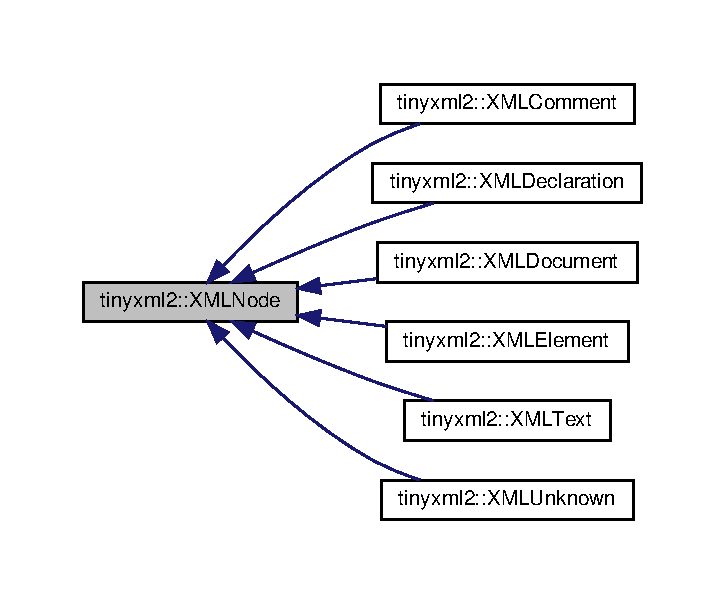
\includegraphics[width=348pt]{classtinyxml2_1_1_x_m_l_node__inherit__graph}
\end{center}
\end{figure}


Collaboration diagram for tinyxml2\+:\+:X\+M\+L\+Node\+:
\nopagebreak
\begin{figure}[H]
\begin{center}
\leavevmode
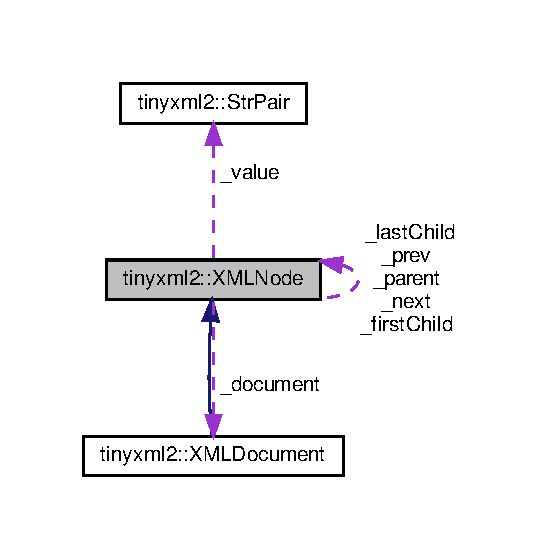
\includegraphics[width=259pt]{classtinyxml2_1_1_x_m_l_node__coll__graph}
\end{center}
\end{figure}
\subsection*{Public Member Functions}
\begin{DoxyCompactItemize}
\item 
\mbox{\Hypertarget{classtinyxml2_1_1_x_m_l_node_a2de84cfa4ec3fe249bad745069d145f1}\label{classtinyxml2_1_1_x_m_l_node_a2de84cfa4ec3fe249bad745069d145f1}} 
const \hyperlink{classtinyxml2_1_1_x_m_l_document}{X\+M\+L\+Document} $\ast$ \hyperlink{classtinyxml2_1_1_x_m_l_node_a2de84cfa4ec3fe249bad745069d145f1}{Get\+Document} () const
\begin{DoxyCompactList}\small\item\em Get the \hyperlink{classtinyxml2_1_1_x_m_l_document}{X\+M\+L\+Document} that owns this \hyperlink{classtinyxml2_1_1_x_m_l_node}{X\+M\+L\+Node}. \end{DoxyCompactList}\item 
\mbox{\Hypertarget{classtinyxml2_1_1_x_m_l_node_af343d1ef0b45c0020e62d784d7e67a68}\label{classtinyxml2_1_1_x_m_l_node_af343d1ef0b45c0020e62d784d7e67a68}} 
\hyperlink{classtinyxml2_1_1_x_m_l_document}{X\+M\+L\+Document} $\ast$ \hyperlink{classtinyxml2_1_1_x_m_l_node_af343d1ef0b45c0020e62d784d7e67a68}{Get\+Document} ()
\begin{DoxyCompactList}\small\item\em Get the \hyperlink{classtinyxml2_1_1_x_m_l_document}{X\+M\+L\+Document} that owns this \hyperlink{classtinyxml2_1_1_x_m_l_node}{X\+M\+L\+Node}. \end{DoxyCompactList}\item 
\mbox{\Hypertarget{classtinyxml2_1_1_x_m_l_node_aab516e699567f75cc9ab2ef2eee501e8}\label{classtinyxml2_1_1_x_m_l_node_aab516e699567f75cc9ab2ef2eee501e8}} 
virtual \hyperlink{classtinyxml2_1_1_x_m_l_element}{X\+M\+L\+Element} $\ast$ \hyperlink{classtinyxml2_1_1_x_m_l_node_aab516e699567f75cc9ab2ef2eee501e8}{To\+Element} ()
\begin{DoxyCompactList}\small\item\em Safely cast to an Element, or null. \end{DoxyCompactList}\item 
\mbox{\Hypertarget{classtinyxml2_1_1_x_m_l_node_a41c55dab9162d1eb62db2008430e376b}\label{classtinyxml2_1_1_x_m_l_node_a41c55dab9162d1eb62db2008430e376b}} 
virtual \hyperlink{classtinyxml2_1_1_x_m_l_text}{X\+M\+L\+Text} $\ast$ \hyperlink{classtinyxml2_1_1_x_m_l_node_a41c55dab9162d1eb62db2008430e376b}{To\+Text} ()
\begin{DoxyCompactList}\small\item\em Safely cast to Text, or null. \end{DoxyCompactList}\item 
\mbox{\Hypertarget{classtinyxml2_1_1_x_m_l_node_aff47671055aa99840a1c1ebd661e63e3}\label{classtinyxml2_1_1_x_m_l_node_aff47671055aa99840a1c1ebd661e63e3}} 
virtual \hyperlink{classtinyxml2_1_1_x_m_l_comment}{X\+M\+L\+Comment} $\ast$ \hyperlink{classtinyxml2_1_1_x_m_l_node_aff47671055aa99840a1c1ebd661e63e3}{To\+Comment} ()
\begin{DoxyCompactList}\small\item\em Safely cast to a Comment, or null. \end{DoxyCompactList}\item 
\mbox{\Hypertarget{classtinyxml2_1_1_x_m_l_node_a836e2966ed736fc3c94f70e12a2a3357}\label{classtinyxml2_1_1_x_m_l_node_a836e2966ed736fc3c94f70e12a2a3357}} 
virtual \hyperlink{classtinyxml2_1_1_x_m_l_document}{X\+M\+L\+Document} $\ast$ \hyperlink{classtinyxml2_1_1_x_m_l_node_a836e2966ed736fc3c94f70e12a2a3357}{To\+Document} ()
\begin{DoxyCompactList}\small\item\em Safely cast to a Document, or null. \end{DoxyCompactList}\item 
\mbox{\Hypertarget{classtinyxml2_1_1_x_m_l_node_a174fd4c22c010b58138c1b84a0dfbd51}\label{classtinyxml2_1_1_x_m_l_node_a174fd4c22c010b58138c1b84a0dfbd51}} 
virtual \hyperlink{classtinyxml2_1_1_x_m_l_declaration}{X\+M\+L\+Declaration} $\ast$ \hyperlink{classtinyxml2_1_1_x_m_l_node_a174fd4c22c010b58138c1b84a0dfbd51}{To\+Declaration} ()
\begin{DoxyCompactList}\small\item\em Safely cast to a Declaration, or null. \end{DoxyCompactList}\item 
\mbox{\Hypertarget{classtinyxml2_1_1_x_m_l_node_a8675a74aa0ada6eccab0c77ef3e5b9bd}\label{classtinyxml2_1_1_x_m_l_node_a8675a74aa0ada6eccab0c77ef3e5b9bd}} 
virtual \hyperlink{classtinyxml2_1_1_x_m_l_unknown}{X\+M\+L\+Unknown} $\ast$ \hyperlink{classtinyxml2_1_1_x_m_l_node_a8675a74aa0ada6eccab0c77ef3e5b9bd}{To\+Unknown} ()
\begin{DoxyCompactList}\small\item\em Safely cast to an Unknown, or null. \end{DoxyCompactList}\item 
\mbox{\Hypertarget{classtinyxml2_1_1_x_m_l_node_a2c5c843b8f37306f15994ebe882b9346}\label{classtinyxml2_1_1_x_m_l_node_a2c5c843b8f37306f15994ebe882b9346}} 
virtual const \hyperlink{classtinyxml2_1_1_x_m_l_element}{X\+M\+L\+Element} $\ast$ {\bfseries To\+Element} () const
\item 
\mbox{\Hypertarget{classtinyxml2_1_1_x_m_l_node_acb9ccc1beda27c0efcb0545683c3e7f4}\label{classtinyxml2_1_1_x_m_l_node_acb9ccc1beda27c0efcb0545683c3e7f4}} 
virtual const \hyperlink{classtinyxml2_1_1_x_m_l_text}{X\+M\+L\+Text} $\ast$ {\bfseries To\+Text} () const
\item 
\mbox{\Hypertarget{classtinyxml2_1_1_x_m_l_node_a6a53bb83faf5c0ccc95b6cf74dba0025}\label{classtinyxml2_1_1_x_m_l_node_a6a53bb83faf5c0ccc95b6cf74dba0025}} 
virtual const \hyperlink{classtinyxml2_1_1_x_m_l_comment}{X\+M\+L\+Comment} $\ast$ {\bfseries To\+Comment} () const
\item 
\mbox{\Hypertarget{classtinyxml2_1_1_x_m_l_node_ae8a5250331a5f12e10843fcb5ef3ef0b}\label{classtinyxml2_1_1_x_m_l_node_ae8a5250331a5f12e10843fcb5ef3ef0b}} 
virtual const \hyperlink{classtinyxml2_1_1_x_m_l_document}{X\+M\+L\+Document} $\ast$ {\bfseries To\+Document} () const
\item 
\mbox{\Hypertarget{classtinyxml2_1_1_x_m_l_node_ac48bb4bf9eb7bb3654ad4b94945db9a1}\label{classtinyxml2_1_1_x_m_l_node_ac48bb4bf9eb7bb3654ad4b94945db9a1}} 
virtual const \hyperlink{classtinyxml2_1_1_x_m_l_declaration}{X\+M\+L\+Declaration} $\ast$ {\bfseries To\+Declaration} () const
\item 
\mbox{\Hypertarget{classtinyxml2_1_1_x_m_l_node_af29ffd6cbe609b6fa04a705256150408}\label{classtinyxml2_1_1_x_m_l_node_af29ffd6cbe609b6fa04a705256150408}} 
virtual const \hyperlink{classtinyxml2_1_1_x_m_l_unknown}{X\+M\+L\+Unknown} $\ast$ {\bfseries To\+Unknown} () const
\item 
const char $\ast$ \hyperlink{classtinyxml2_1_1_x_m_l_node_a0485e51c670e741884cfd8362274d680}{Value} () const
\item 
void \hyperlink{classtinyxml2_1_1_x_m_l_node_a09dd68cf9eae137579f6e50f36487513}{Set\+Value} (const char $\ast$val, bool static\+Mem=false)
\item 
\mbox{\Hypertarget{classtinyxml2_1_1_x_m_l_node_a9b5fc636646fda761d342c72e91cb286}\label{classtinyxml2_1_1_x_m_l_node_a9b5fc636646fda761d342c72e91cb286}} 
int \hyperlink{classtinyxml2_1_1_x_m_l_node_a9b5fc636646fda761d342c72e91cb286}{Get\+Line\+Num} () const
\begin{DoxyCompactList}\small\item\em Gets the line number the node is in, if the document was parsed from a file. \end{DoxyCompactList}\item 
\mbox{\Hypertarget{classtinyxml2_1_1_x_m_l_node_ae0f62bc186c56c2e0483ebd52dbfbe34}\label{classtinyxml2_1_1_x_m_l_node_ae0f62bc186c56c2e0483ebd52dbfbe34}} 
const \hyperlink{classtinyxml2_1_1_x_m_l_node}{X\+M\+L\+Node} $\ast$ \hyperlink{classtinyxml2_1_1_x_m_l_node_ae0f62bc186c56c2e0483ebd52dbfbe34}{Parent} () const
\begin{DoxyCompactList}\small\item\em Get the parent of this node on the D\+OM. \end{DoxyCompactList}\item 
\mbox{\Hypertarget{classtinyxml2_1_1_x_m_l_node_a76029693a5a54fbb721a41d7a0ca8a97}\label{classtinyxml2_1_1_x_m_l_node_a76029693a5a54fbb721a41d7a0ca8a97}} 
\hyperlink{classtinyxml2_1_1_x_m_l_node}{X\+M\+L\+Node} $\ast$ {\bfseries Parent} ()
\item 
\mbox{\Hypertarget{classtinyxml2_1_1_x_m_l_node_ac3ab489e6e202a3cd1762d3b332e89d4}\label{classtinyxml2_1_1_x_m_l_node_ac3ab489e6e202a3cd1762d3b332e89d4}} 
bool \hyperlink{classtinyxml2_1_1_x_m_l_node_ac3ab489e6e202a3cd1762d3b332e89d4}{No\+Children} () const
\begin{DoxyCompactList}\small\item\em Returns true if this node has no children. \end{DoxyCompactList}\item 
\mbox{\Hypertarget{classtinyxml2_1_1_x_m_l_node_ae7dc225e1018cdd685f7563593a1fe08}\label{classtinyxml2_1_1_x_m_l_node_ae7dc225e1018cdd685f7563593a1fe08}} 
const \hyperlink{classtinyxml2_1_1_x_m_l_node}{X\+M\+L\+Node} $\ast$ \hyperlink{classtinyxml2_1_1_x_m_l_node_ae7dc225e1018cdd685f7563593a1fe08}{First\+Child} () const
\begin{DoxyCompactList}\small\item\em Get the first child node, or null if none exists. \end{DoxyCompactList}\item 
\mbox{\Hypertarget{classtinyxml2_1_1_x_m_l_node_a2d6c70c475146b48bc93a7fafdeff5e0}\label{classtinyxml2_1_1_x_m_l_node_a2d6c70c475146b48bc93a7fafdeff5e0}} 
\hyperlink{classtinyxml2_1_1_x_m_l_node}{X\+M\+L\+Node} $\ast$ {\bfseries First\+Child} ()
\item 
const \hyperlink{classtinyxml2_1_1_x_m_l_element}{X\+M\+L\+Element} $\ast$ \hyperlink{classtinyxml2_1_1_x_m_l_node_a1bec132dcf085284e0a10755f2cf0d57}{First\+Child\+Element} (const char $\ast$name=0) const
\item 
\mbox{\Hypertarget{classtinyxml2_1_1_x_m_l_node_af1e0e475cc27d5e7eeaf4d732691b741}\label{classtinyxml2_1_1_x_m_l_node_af1e0e475cc27d5e7eeaf4d732691b741}} 
\hyperlink{classtinyxml2_1_1_x_m_l_element}{X\+M\+L\+Element} $\ast$ {\bfseries First\+Child\+Element} (const char $\ast$name=0)
\item 
\mbox{\Hypertarget{classtinyxml2_1_1_x_m_l_node_a9b8583a277e8e26f4cbbb5492786778e}\label{classtinyxml2_1_1_x_m_l_node_a9b8583a277e8e26f4cbbb5492786778e}} 
const \hyperlink{classtinyxml2_1_1_x_m_l_node}{X\+M\+L\+Node} $\ast$ \hyperlink{classtinyxml2_1_1_x_m_l_node_a9b8583a277e8e26f4cbbb5492786778e}{Last\+Child} () const
\begin{DoxyCompactList}\small\item\em Get the last child node, or null if none exists. \end{DoxyCompactList}\item 
\mbox{\Hypertarget{classtinyxml2_1_1_x_m_l_node_ad7552c8cb1dc0cb6f3bdc14a9d115dbf}\label{classtinyxml2_1_1_x_m_l_node_ad7552c8cb1dc0cb6f3bdc14a9d115dbf}} 
\hyperlink{classtinyxml2_1_1_x_m_l_node}{X\+M\+L\+Node} $\ast$ {\bfseries Last\+Child} ()
\item 
const \hyperlink{classtinyxml2_1_1_x_m_l_element}{X\+M\+L\+Element} $\ast$ \hyperlink{classtinyxml2_1_1_x_m_l_node_a609e02f02044f39b928d1a3e0de9f532}{Last\+Child\+Element} (const char $\ast$name=0) const
\item 
\mbox{\Hypertarget{classtinyxml2_1_1_x_m_l_node_a1b77a8194d059665a4412ebfea276878}\label{classtinyxml2_1_1_x_m_l_node_a1b77a8194d059665a4412ebfea276878}} 
\hyperlink{classtinyxml2_1_1_x_m_l_element}{X\+M\+L\+Element} $\ast$ {\bfseries Last\+Child\+Element} (const char $\ast$name=0)
\item 
\mbox{\Hypertarget{classtinyxml2_1_1_x_m_l_node_aac667c513d445f8b783e1e15ef9d3551}\label{classtinyxml2_1_1_x_m_l_node_aac667c513d445f8b783e1e15ef9d3551}} 
const \hyperlink{classtinyxml2_1_1_x_m_l_node}{X\+M\+L\+Node} $\ast$ \hyperlink{classtinyxml2_1_1_x_m_l_node_aac667c513d445f8b783e1e15ef9d3551}{Previous\+Sibling} () const
\begin{DoxyCompactList}\small\item\em Get the previous (left) sibling node of this node. \end{DoxyCompactList}\item 
\mbox{\Hypertarget{classtinyxml2_1_1_x_m_l_node_ae760e5e7e766df1d2cf3bb4a847876d6}\label{classtinyxml2_1_1_x_m_l_node_ae760e5e7e766df1d2cf3bb4a847876d6}} 
\hyperlink{classtinyxml2_1_1_x_m_l_node}{X\+M\+L\+Node} $\ast$ {\bfseries Previous\+Sibling} ()
\item 
\mbox{\Hypertarget{classtinyxml2_1_1_x_m_l_node_a9453cda5e970375a7b1b2099f8a7c40a}\label{classtinyxml2_1_1_x_m_l_node_a9453cda5e970375a7b1b2099f8a7c40a}} 
const \hyperlink{classtinyxml2_1_1_x_m_l_element}{X\+M\+L\+Element} $\ast$ \hyperlink{classtinyxml2_1_1_x_m_l_node_a9453cda5e970375a7b1b2099f8a7c40a}{Previous\+Sibling\+Element} (const char $\ast$name=0) const
\begin{DoxyCompactList}\small\item\em Get the previous (left) sibling element of this node, with an optionally supplied name. \end{DoxyCompactList}\item 
\mbox{\Hypertarget{classtinyxml2_1_1_x_m_l_node_ae4f37eb6cd405bdf1d57caa066e36d87}\label{classtinyxml2_1_1_x_m_l_node_ae4f37eb6cd405bdf1d57caa066e36d87}} 
\hyperlink{classtinyxml2_1_1_x_m_l_element}{X\+M\+L\+Element} $\ast$ {\bfseries Previous\+Sibling\+Element} (const char $\ast$name=0)
\item 
\mbox{\Hypertarget{classtinyxml2_1_1_x_m_l_node_a79db9ef0fe014d27790f2218b87bcbb5}\label{classtinyxml2_1_1_x_m_l_node_a79db9ef0fe014d27790f2218b87bcbb5}} 
const \hyperlink{classtinyxml2_1_1_x_m_l_node}{X\+M\+L\+Node} $\ast$ \hyperlink{classtinyxml2_1_1_x_m_l_node_a79db9ef0fe014d27790f2218b87bcbb5}{Next\+Sibling} () const
\begin{DoxyCompactList}\small\item\em Get the next (right) sibling node of this node. \end{DoxyCompactList}\item 
\mbox{\Hypertarget{classtinyxml2_1_1_x_m_l_node_aeb7d4dfd8fb924ef86e7cb72183acbac}\label{classtinyxml2_1_1_x_m_l_node_aeb7d4dfd8fb924ef86e7cb72183acbac}} 
\hyperlink{classtinyxml2_1_1_x_m_l_node}{X\+M\+L\+Node} $\ast$ {\bfseries Next\+Sibling} ()
\item 
\mbox{\Hypertarget{classtinyxml2_1_1_x_m_l_node_a14ea560df31110ff07a9f566171bf797}\label{classtinyxml2_1_1_x_m_l_node_a14ea560df31110ff07a9f566171bf797}} 
const \hyperlink{classtinyxml2_1_1_x_m_l_element}{X\+M\+L\+Element} $\ast$ \hyperlink{classtinyxml2_1_1_x_m_l_node_a14ea560df31110ff07a9f566171bf797}{Next\+Sibling\+Element} (const char $\ast$name=0) const
\begin{DoxyCompactList}\small\item\em Get the next (right) sibling element of this node, with an optionally supplied name. \end{DoxyCompactList}\item 
\mbox{\Hypertarget{classtinyxml2_1_1_x_m_l_node_af1225412584d4a2126f55e96a12e0ec0}\label{classtinyxml2_1_1_x_m_l_node_af1225412584d4a2126f55e96a12e0ec0}} 
\hyperlink{classtinyxml2_1_1_x_m_l_element}{X\+M\+L\+Element} $\ast$ {\bfseries Next\+Sibling\+Element} (const char $\ast$name=0)
\item 
\hyperlink{classtinyxml2_1_1_x_m_l_node}{X\+M\+L\+Node} $\ast$ \hyperlink{classtinyxml2_1_1_x_m_l_node_ae3b422e98914d6002ca99bb1d2837103}{Insert\+End\+Child} (\hyperlink{classtinyxml2_1_1_x_m_l_node}{X\+M\+L\+Node} $\ast$add\+This)
\item 
\mbox{\Hypertarget{classtinyxml2_1_1_x_m_l_node_a663e3a5a378169fd477378f4d17a7649}\label{classtinyxml2_1_1_x_m_l_node_a663e3a5a378169fd477378f4d17a7649}} 
\hyperlink{classtinyxml2_1_1_x_m_l_node}{X\+M\+L\+Node} $\ast$ {\bfseries Link\+End\+Child} (\hyperlink{classtinyxml2_1_1_x_m_l_node}{X\+M\+L\+Node} $\ast$add\+This)
\item 
\hyperlink{classtinyxml2_1_1_x_m_l_node}{X\+M\+L\+Node} $\ast$ \hyperlink{classtinyxml2_1_1_x_m_l_node_ac609a8f3ea949027f439280c640bbaf2}{Insert\+First\+Child} (\hyperlink{classtinyxml2_1_1_x_m_l_node}{X\+M\+L\+Node} $\ast$add\+This)
\item 
\hyperlink{classtinyxml2_1_1_x_m_l_node}{X\+M\+L\+Node} $\ast$ \hyperlink{classtinyxml2_1_1_x_m_l_node_a9275138a1b8dd5d8e2c26789bdc23ac8}{Insert\+After\+Child} (\hyperlink{classtinyxml2_1_1_x_m_l_node}{X\+M\+L\+Node} $\ast$after\+This, \hyperlink{classtinyxml2_1_1_x_m_l_node}{X\+M\+L\+Node} $\ast$add\+This)
\item 
void \hyperlink{classtinyxml2_1_1_x_m_l_node_a0360085cc54df5bff85d5c5da13afdce}{Delete\+Children} ()
\item 
void \hyperlink{classtinyxml2_1_1_x_m_l_node_a363b6edbd6ebd55f8387d2b89f2b0921}{Delete\+Child} (\hyperlink{classtinyxml2_1_1_x_m_l_node}{X\+M\+L\+Node} $\ast$node)
\item 
virtual \hyperlink{classtinyxml2_1_1_x_m_l_node}{X\+M\+L\+Node} $\ast$ \hyperlink{classtinyxml2_1_1_x_m_l_node_a8402cbd3129d20e9e6024bbcc0531283}{Shallow\+Clone} (\hyperlink{classtinyxml2_1_1_x_m_l_document}{X\+M\+L\+Document} $\ast$document) const =0
\item 
\hyperlink{classtinyxml2_1_1_x_m_l_node}{X\+M\+L\+Node} $\ast$ \hyperlink{classtinyxml2_1_1_x_m_l_node_a3bb369fd733f1989b751d99a9417adab}{Deep\+Clone} (\hyperlink{classtinyxml2_1_1_x_m_l_document}{X\+M\+L\+Document} $\ast$target) const
\item 
virtual bool \hyperlink{classtinyxml2_1_1_x_m_l_node_a7ce18b751c3ea09eac292dca264f9226}{Shallow\+Equal} (const \hyperlink{classtinyxml2_1_1_x_m_l_node}{X\+M\+L\+Node} $\ast$compare) const =0
\item 
virtual bool \hyperlink{classtinyxml2_1_1_x_m_l_node_a81e66df0a44c67a7af17f3b77a152785}{Accept} (\hyperlink{classtinyxml2_1_1_x_m_l_visitor}{X\+M\+L\+Visitor} $\ast$visitor) const =0
\item 
void \hyperlink{classtinyxml2_1_1_x_m_l_node_a002978fc889cc011d143185f2377eca2}{Set\+User\+Data} (void $\ast$user\+Data)
\item 
void $\ast$ \hyperlink{classtinyxml2_1_1_x_m_l_node_a7f0687574afa03bc479dc44f29db0afe}{Get\+User\+Data} () const
\end{DoxyCompactItemize}
\subsection*{Protected Member Functions}
\begin{DoxyCompactItemize}
\item 
\mbox{\Hypertarget{classtinyxml2_1_1_x_m_l_node_a29868df6ca383d574f584dfdd15105b6}\label{classtinyxml2_1_1_x_m_l_node_a29868df6ca383d574f584dfdd15105b6}} 
{\bfseries X\+M\+L\+Node} (\hyperlink{classtinyxml2_1_1_x_m_l_document}{X\+M\+L\+Document} $\ast$)
\item 
\mbox{\Hypertarget{classtinyxml2_1_1_x_m_l_node_a916e498914baecbc9a1f012352ef7c69}\label{classtinyxml2_1_1_x_m_l_node_a916e498914baecbc9a1f012352ef7c69}} 
virtual char $\ast$ {\bfseries Parse\+Deep} (char $\ast$p, \hyperlink{classtinyxml2_1_1_str_pair}{Str\+Pair} $\ast$parent\+End\+Tag, int $\ast$cur\+Line\+Num\+Ptr)
\end{DoxyCompactItemize}
\subsection*{Protected Attributes}
\begin{DoxyCompactItemize}
\item 
\mbox{\Hypertarget{classtinyxml2_1_1_x_m_l_node_a8d2d2be0bb6797625551eb0e91f0ff62}\label{classtinyxml2_1_1_x_m_l_node_a8d2d2be0bb6797625551eb0e91f0ff62}} 
\hyperlink{classtinyxml2_1_1_x_m_l_document}{X\+M\+L\+Document} $\ast$ {\bfseries \+\_\+document}
\item 
\mbox{\Hypertarget{classtinyxml2_1_1_x_m_l_node_a176dd1c4965c21c366de192164aa2c13}\label{classtinyxml2_1_1_x_m_l_node_a176dd1c4965c21c366de192164aa2c13}} 
\hyperlink{classtinyxml2_1_1_x_m_l_node}{X\+M\+L\+Node} $\ast$ {\bfseries \+\_\+parent}
\item 
\mbox{\Hypertarget{classtinyxml2_1_1_x_m_l_node_a3ea9884098b8379de2bb5ab3fc85c0fc}\label{classtinyxml2_1_1_x_m_l_node_a3ea9884098b8379de2bb5ab3fc85c0fc}} 
\hyperlink{classtinyxml2_1_1_str_pair}{Str\+Pair} {\bfseries \+\_\+value}
\item 
\mbox{\Hypertarget{classtinyxml2_1_1_x_m_l_node_ab336ed023e15be202ff3b410be01b804}\label{classtinyxml2_1_1_x_m_l_node_ab336ed023e15be202ff3b410be01b804}} 
int {\bfseries \+\_\+parse\+Line\+Num}
\item 
\mbox{\Hypertarget{classtinyxml2_1_1_x_m_l_node_aa20c91e4213dc930c5bdf420322ca342}\label{classtinyxml2_1_1_x_m_l_node_aa20c91e4213dc930c5bdf420322ca342}} 
\hyperlink{classtinyxml2_1_1_x_m_l_node}{X\+M\+L\+Node} $\ast$ {\bfseries \+\_\+first\+Child}
\item 
\mbox{\Hypertarget{classtinyxml2_1_1_x_m_l_node_a099b6560ae44ab9edb8453aaf1a3747b}\label{classtinyxml2_1_1_x_m_l_node_a099b6560ae44ab9edb8453aaf1a3747b}} 
\hyperlink{classtinyxml2_1_1_x_m_l_node}{X\+M\+L\+Node} $\ast$ {\bfseries \+\_\+last\+Child}
\item 
\mbox{\Hypertarget{classtinyxml2_1_1_x_m_l_node_a9739eb0fb9a1188266052055e7a6bf6b}\label{classtinyxml2_1_1_x_m_l_node_a9739eb0fb9a1188266052055e7a6bf6b}} 
\hyperlink{classtinyxml2_1_1_x_m_l_node}{X\+M\+L\+Node} $\ast$ {\bfseries \+\_\+prev}
\item 
\mbox{\Hypertarget{classtinyxml2_1_1_x_m_l_node_a27e985496b37dd00eb5b9cf59b9e3fb1}\label{classtinyxml2_1_1_x_m_l_node_a27e985496b37dd00eb5b9cf59b9e3fb1}} 
\hyperlink{classtinyxml2_1_1_x_m_l_node}{X\+M\+L\+Node} $\ast$ {\bfseries \+\_\+next}
\item 
\mbox{\Hypertarget{classtinyxml2_1_1_x_m_l_node_ac2d5cc463a6c95ec5907d57a119c56da}\label{classtinyxml2_1_1_x_m_l_node_ac2d5cc463a6c95ec5907d57a119c56da}} 
void $\ast$ {\bfseries \+\_\+user\+Data}
\end{DoxyCompactItemize}
\subsection*{Friends}
\begin{DoxyCompactItemize}
\item 
\mbox{\Hypertarget{classtinyxml2_1_1_x_m_l_node_a4eee3bda60c60a30e4e8cd4ea91c4c6e}\label{classtinyxml2_1_1_x_m_l_node_a4eee3bda60c60a30e4e8cd4ea91c4c6e}} 
class {\bfseries X\+M\+L\+Document}
\item 
\mbox{\Hypertarget{classtinyxml2_1_1_x_m_l_node_ac2fba9b6e452829dd892f7392c24e0eb}\label{classtinyxml2_1_1_x_m_l_node_ac2fba9b6e452829dd892f7392c24e0eb}} 
class {\bfseries X\+M\+L\+Element}
\end{DoxyCompactItemize}


\subsection{Detailed Description}
\hyperlink{classtinyxml2_1_1_x_m_l_node}{X\+M\+L\+Node} is a base class for every object that is in the X\+ML Document Object Model (D\+OM), except X\+M\+L\+Attributes. Nodes have siblings, a parent, and children which can be navigated. A node is always in a \hyperlink{classtinyxml2_1_1_x_m_l_document}{X\+M\+L\+Document}. The type of a \hyperlink{classtinyxml2_1_1_x_m_l_node}{X\+M\+L\+Node} can be queried, and it can be cast to its more defined type.

A \hyperlink{classtinyxml2_1_1_x_m_l_document}{X\+M\+L\+Document} allocates memory for all its Nodes. When the \hyperlink{classtinyxml2_1_1_x_m_l_document}{X\+M\+L\+Document} gets deleted, all its Nodes will also be deleted.

\begin{DoxyVerb}A Document can contain: Element (container or leaf)
                        Comment (leaf)
                        Unknown (leaf)
                        Declaration( leaf )

An Element can contain: Element (container or leaf)
                        Text    (leaf)
                        Attributes (not on tree)
                        Comment (leaf)
                        Unknown (leaf)\end{DoxyVerb}
 

\subsection{Member Function Documentation}
\mbox{\Hypertarget{classtinyxml2_1_1_x_m_l_node_a81e66df0a44c67a7af17f3b77a152785}\label{classtinyxml2_1_1_x_m_l_node_a81e66df0a44c67a7af17f3b77a152785}} 
\index{tinyxml2\+::\+X\+M\+L\+Node@{tinyxml2\+::\+X\+M\+L\+Node}!Accept@{Accept}}
\index{Accept@{Accept}!tinyxml2\+::\+X\+M\+L\+Node@{tinyxml2\+::\+X\+M\+L\+Node}}
\subsubsection{\texorpdfstring{Accept()}{Accept()}}
{\footnotesize\ttfamily virtual bool tinyxml2\+::\+X\+M\+L\+Node\+::\+Accept (\begin{DoxyParamCaption}\item[{\hyperlink{classtinyxml2_1_1_x_m_l_visitor}{X\+M\+L\+Visitor} $\ast$}]{visitor }\end{DoxyParamCaption}) const\hspace{0.3cm}{\ttfamily [pure virtual]}}

Accept a hierarchical visit of the nodes in the Tiny\+X\+M\+L-\/2 D\+OM. Every node in the X\+ML tree will be conditionally visited and the host will be called back via the \hyperlink{classtinyxml2_1_1_x_m_l_visitor}{X\+M\+L\+Visitor} interface.

This is essentially a S\+AX interface for Tiny\+X\+M\+L-\/2. (Note however it doesn\textquotesingle{}t re-\/parse the X\+ML for the callbacks, so the performance of Tiny\+X\+M\+L-\/2 is unchanged by using this interface versus any other.)

The interface has been based on ideas from\+:


\begin{DoxyItemize}
\item \href{http://www.saxproject.org/}{\tt http\+://www.\+saxproject.\+org/}
\item \href{http://c2.com/cgi/wiki?HierarchicalVisitorPattern}{\tt http\+://c2.\+com/cgi/wiki?\+Hierarchical\+Visitor\+Pattern}
\end{DoxyItemize}

Which are both good references for \char`\"{}visiting\char`\"{}.

An example of using \hyperlink{classtinyxml2_1_1_x_m_l_node_a81e66df0a44c67a7af17f3b77a152785}{Accept()}\+: \begin{DoxyVerb}XMLPrinter printer;
tinyxmlDoc.Accept( &printer );
const char* xmlcstr = printer.CStr();
\end{DoxyVerb}
 

Implemented in \hyperlink{classtinyxml2_1_1_x_m_l_document_ab7be651917a35ab1ff0e4e6d4e565cdf}{tinyxml2\+::\+X\+M\+L\+Document}, \hyperlink{classtinyxml2_1_1_x_m_l_element_a9b2119831e8b85827d5d3e5076788e4a}{tinyxml2\+::\+X\+M\+L\+Element}, \hyperlink{classtinyxml2_1_1_x_m_l_unknown_a8a06b8c82117ca969a432e17a46830fc}{tinyxml2\+::\+X\+M\+L\+Unknown}, \hyperlink{classtinyxml2_1_1_x_m_l_declaration_acf47629d9fc08ed6f1c164a97bcf794b}{tinyxml2\+::\+X\+M\+L\+Declaration}, \hyperlink{classtinyxml2_1_1_x_m_l_comment_a27b37d16cea01b5329dfbbb4f9508e39}{tinyxml2\+::\+X\+M\+L\+Comment}, and \hyperlink{classtinyxml2_1_1_x_m_l_text_a537c60d7e18fb59c45ac2737a29ac47a}{tinyxml2\+::\+X\+M\+L\+Text}.

\mbox{\Hypertarget{classtinyxml2_1_1_x_m_l_node_a3bb369fd733f1989b751d99a9417adab}\label{classtinyxml2_1_1_x_m_l_node_a3bb369fd733f1989b751d99a9417adab}} 
\index{tinyxml2\+::\+X\+M\+L\+Node@{tinyxml2\+::\+X\+M\+L\+Node}!Deep\+Clone@{Deep\+Clone}}
\index{Deep\+Clone@{Deep\+Clone}!tinyxml2\+::\+X\+M\+L\+Node@{tinyxml2\+::\+X\+M\+L\+Node}}
\subsubsection{\texorpdfstring{Deep\+Clone()}{DeepClone()}}
{\footnotesize\ttfamily \hyperlink{classtinyxml2_1_1_x_m_l_node}{X\+M\+L\+Node} $\ast$ tinyxml2\+::\+X\+M\+L\+Node\+::\+Deep\+Clone (\begin{DoxyParamCaption}\item[{\hyperlink{classtinyxml2_1_1_x_m_l_document}{X\+M\+L\+Document} $\ast$}]{target }\end{DoxyParamCaption}) const}

Make a copy of this node and all its children.

If the \textquotesingle{}target\textquotesingle{} is null, then the nodes will be allocated in the current document. If \textquotesingle{}target\textquotesingle{} is specified, the memory will be allocated is the specified \hyperlink{classtinyxml2_1_1_x_m_l_document}{X\+M\+L\+Document}.

N\+O\+TE\+: This is probably not the correct tool to copy a document, since X\+M\+L\+Documents can have multiple top level X\+M\+L\+Nodes. You probably want to use \hyperlink{classtinyxml2_1_1_x_m_l_document_af592ffc91514e25a39664521ac83db45}{X\+M\+L\+Document\+::\+Deep\+Copy()} \mbox{\Hypertarget{classtinyxml2_1_1_x_m_l_node_a363b6edbd6ebd55f8387d2b89f2b0921}\label{classtinyxml2_1_1_x_m_l_node_a363b6edbd6ebd55f8387d2b89f2b0921}} 
\index{tinyxml2\+::\+X\+M\+L\+Node@{tinyxml2\+::\+X\+M\+L\+Node}!Delete\+Child@{Delete\+Child}}
\index{Delete\+Child@{Delete\+Child}!tinyxml2\+::\+X\+M\+L\+Node@{tinyxml2\+::\+X\+M\+L\+Node}}
\subsubsection{\texorpdfstring{Delete\+Child()}{DeleteChild()}}
{\footnotesize\ttfamily void tinyxml2\+::\+X\+M\+L\+Node\+::\+Delete\+Child (\begin{DoxyParamCaption}\item[{\hyperlink{classtinyxml2_1_1_x_m_l_node}{X\+M\+L\+Node} $\ast$}]{node }\end{DoxyParamCaption})}

Delete a child of this node. \mbox{\Hypertarget{classtinyxml2_1_1_x_m_l_node_a0360085cc54df5bff85d5c5da13afdce}\label{classtinyxml2_1_1_x_m_l_node_a0360085cc54df5bff85d5c5da13afdce}} 
\index{tinyxml2\+::\+X\+M\+L\+Node@{tinyxml2\+::\+X\+M\+L\+Node}!Delete\+Children@{Delete\+Children}}
\index{Delete\+Children@{Delete\+Children}!tinyxml2\+::\+X\+M\+L\+Node@{tinyxml2\+::\+X\+M\+L\+Node}}
\subsubsection{\texorpdfstring{Delete\+Children()}{DeleteChildren()}}
{\footnotesize\ttfamily void tinyxml2\+::\+X\+M\+L\+Node\+::\+Delete\+Children (\begin{DoxyParamCaption}{ }\end{DoxyParamCaption})}

Delete all the children of this node. \mbox{\Hypertarget{classtinyxml2_1_1_x_m_l_node_a1bec132dcf085284e0a10755f2cf0d57}\label{classtinyxml2_1_1_x_m_l_node_a1bec132dcf085284e0a10755f2cf0d57}} 
\index{tinyxml2\+::\+X\+M\+L\+Node@{tinyxml2\+::\+X\+M\+L\+Node}!First\+Child\+Element@{First\+Child\+Element}}
\index{First\+Child\+Element@{First\+Child\+Element}!tinyxml2\+::\+X\+M\+L\+Node@{tinyxml2\+::\+X\+M\+L\+Node}}
\subsubsection{\texorpdfstring{First\+Child\+Element()}{FirstChildElement()}}
{\footnotesize\ttfamily const \hyperlink{classtinyxml2_1_1_x_m_l_element}{X\+M\+L\+Element} $\ast$ tinyxml2\+::\+X\+M\+L\+Node\+::\+First\+Child\+Element (\begin{DoxyParamCaption}\item[{const char $\ast$}]{name = {\ttfamily 0} }\end{DoxyParamCaption}) const}

Get the first child element, or optionally the first child element with the specified name. \mbox{\Hypertarget{classtinyxml2_1_1_x_m_l_node_a7f0687574afa03bc479dc44f29db0afe}\label{classtinyxml2_1_1_x_m_l_node_a7f0687574afa03bc479dc44f29db0afe}} 
\index{tinyxml2\+::\+X\+M\+L\+Node@{tinyxml2\+::\+X\+M\+L\+Node}!Get\+User\+Data@{Get\+User\+Data}}
\index{Get\+User\+Data@{Get\+User\+Data}!tinyxml2\+::\+X\+M\+L\+Node@{tinyxml2\+::\+X\+M\+L\+Node}}
\subsubsection{\texorpdfstring{Get\+User\+Data()}{GetUserData()}}
{\footnotesize\ttfamily void$\ast$ tinyxml2\+::\+X\+M\+L\+Node\+::\+Get\+User\+Data (\begin{DoxyParamCaption}{ }\end{DoxyParamCaption}) const\hspace{0.3cm}{\ttfamily [inline]}}

Get user data set into the \hyperlink{classtinyxml2_1_1_x_m_l_node}{X\+M\+L\+Node}. Tiny\+X\+M\+L-\/2 in no way processes or interprets user data. It is initially 0. \mbox{\Hypertarget{classtinyxml2_1_1_x_m_l_node_a9275138a1b8dd5d8e2c26789bdc23ac8}\label{classtinyxml2_1_1_x_m_l_node_a9275138a1b8dd5d8e2c26789bdc23ac8}} 
\index{tinyxml2\+::\+X\+M\+L\+Node@{tinyxml2\+::\+X\+M\+L\+Node}!Insert\+After\+Child@{Insert\+After\+Child}}
\index{Insert\+After\+Child@{Insert\+After\+Child}!tinyxml2\+::\+X\+M\+L\+Node@{tinyxml2\+::\+X\+M\+L\+Node}}
\subsubsection{\texorpdfstring{Insert\+After\+Child()}{InsertAfterChild()}}
{\footnotesize\ttfamily \hyperlink{classtinyxml2_1_1_x_m_l_node}{X\+M\+L\+Node} $\ast$ tinyxml2\+::\+X\+M\+L\+Node\+::\+Insert\+After\+Child (\begin{DoxyParamCaption}\item[{\hyperlink{classtinyxml2_1_1_x_m_l_node}{X\+M\+L\+Node} $\ast$}]{after\+This,  }\item[{\hyperlink{classtinyxml2_1_1_x_m_l_node}{X\+M\+L\+Node} $\ast$}]{add\+This }\end{DoxyParamCaption})}

Add a node after the specified child node. If the child node is already part of the document, it is moved from its old location to the new location. Returns the add\+This argument or 0 if the after\+This node is not a child of this node, or if the node does not belong to the same document. \mbox{\Hypertarget{classtinyxml2_1_1_x_m_l_node_ae3b422e98914d6002ca99bb1d2837103}\label{classtinyxml2_1_1_x_m_l_node_ae3b422e98914d6002ca99bb1d2837103}} 
\index{tinyxml2\+::\+X\+M\+L\+Node@{tinyxml2\+::\+X\+M\+L\+Node}!Insert\+End\+Child@{Insert\+End\+Child}}
\index{Insert\+End\+Child@{Insert\+End\+Child}!tinyxml2\+::\+X\+M\+L\+Node@{tinyxml2\+::\+X\+M\+L\+Node}}
\subsubsection{\texorpdfstring{Insert\+End\+Child()}{InsertEndChild()}}
{\footnotesize\ttfamily \hyperlink{classtinyxml2_1_1_x_m_l_node}{X\+M\+L\+Node} $\ast$ tinyxml2\+::\+X\+M\+L\+Node\+::\+Insert\+End\+Child (\begin{DoxyParamCaption}\item[{\hyperlink{classtinyxml2_1_1_x_m_l_node}{X\+M\+L\+Node} $\ast$}]{add\+This }\end{DoxyParamCaption})}

Add a child node as the last (right) child. If the child node is already part of the document, it is moved from its old location to the new location. Returns the add\+This argument or 0 if the node does not belong to the same document. \mbox{\Hypertarget{classtinyxml2_1_1_x_m_l_node_ac609a8f3ea949027f439280c640bbaf2}\label{classtinyxml2_1_1_x_m_l_node_ac609a8f3ea949027f439280c640bbaf2}} 
\index{tinyxml2\+::\+X\+M\+L\+Node@{tinyxml2\+::\+X\+M\+L\+Node}!Insert\+First\+Child@{Insert\+First\+Child}}
\index{Insert\+First\+Child@{Insert\+First\+Child}!tinyxml2\+::\+X\+M\+L\+Node@{tinyxml2\+::\+X\+M\+L\+Node}}
\subsubsection{\texorpdfstring{Insert\+First\+Child()}{InsertFirstChild()}}
{\footnotesize\ttfamily \hyperlink{classtinyxml2_1_1_x_m_l_node}{X\+M\+L\+Node} $\ast$ tinyxml2\+::\+X\+M\+L\+Node\+::\+Insert\+First\+Child (\begin{DoxyParamCaption}\item[{\hyperlink{classtinyxml2_1_1_x_m_l_node}{X\+M\+L\+Node} $\ast$}]{add\+This }\end{DoxyParamCaption})}

Add a child node as the first (left) child. If the child node is already part of the document, it is moved from its old location to the new location. Returns the add\+This argument or 0 if the node does not belong to the same document. \mbox{\Hypertarget{classtinyxml2_1_1_x_m_l_node_a609e02f02044f39b928d1a3e0de9f532}\label{classtinyxml2_1_1_x_m_l_node_a609e02f02044f39b928d1a3e0de9f532}} 
\index{tinyxml2\+::\+X\+M\+L\+Node@{tinyxml2\+::\+X\+M\+L\+Node}!Last\+Child\+Element@{Last\+Child\+Element}}
\index{Last\+Child\+Element@{Last\+Child\+Element}!tinyxml2\+::\+X\+M\+L\+Node@{tinyxml2\+::\+X\+M\+L\+Node}}
\subsubsection{\texorpdfstring{Last\+Child\+Element()}{LastChildElement()}}
{\footnotesize\ttfamily const \hyperlink{classtinyxml2_1_1_x_m_l_element}{X\+M\+L\+Element} $\ast$ tinyxml2\+::\+X\+M\+L\+Node\+::\+Last\+Child\+Element (\begin{DoxyParamCaption}\item[{const char $\ast$}]{name = {\ttfamily 0} }\end{DoxyParamCaption}) const}

Get the last child element or optionally the last child element with the specified name. \mbox{\Hypertarget{classtinyxml2_1_1_x_m_l_node_a002978fc889cc011d143185f2377eca2}\label{classtinyxml2_1_1_x_m_l_node_a002978fc889cc011d143185f2377eca2}} 
\index{tinyxml2\+::\+X\+M\+L\+Node@{tinyxml2\+::\+X\+M\+L\+Node}!Set\+User\+Data@{Set\+User\+Data}}
\index{Set\+User\+Data@{Set\+User\+Data}!tinyxml2\+::\+X\+M\+L\+Node@{tinyxml2\+::\+X\+M\+L\+Node}}
\subsubsection{\texorpdfstring{Set\+User\+Data()}{SetUserData()}}
{\footnotesize\ttfamily void tinyxml2\+::\+X\+M\+L\+Node\+::\+Set\+User\+Data (\begin{DoxyParamCaption}\item[{void $\ast$}]{user\+Data }\end{DoxyParamCaption})\hspace{0.3cm}{\ttfamily [inline]}}

Set user data into the \hyperlink{classtinyxml2_1_1_x_m_l_node}{X\+M\+L\+Node}. Tiny\+X\+M\+L-\/2 in no way processes or interprets user data. It is initially 0. \mbox{\Hypertarget{classtinyxml2_1_1_x_m_l_node_a09dd68cf9eae137579f6e50f36487513}\label{classtinyxml2_1_1_x_m_l_node_a09dd68cf9eae137579f6e50f36487513}} 
\index{tinyxml2\+::\+X\+M\+L\+Node@{tinyxml2\+::\+X\+M\+L\+Node}!Set\+Value@{Set\+Value}}
\index{Set\+Value@{Set\+Value}!tinyxml2\+::\+X\+M\+L\+Node@{tinyxml2\+::\+X\+M\+L\+Node}}
\subsubsection{\texorpdfstring{Set\+Value()}{SetValue()}}
{\footnotesize\ttfamily void tinyxml2\+::\+X\+M\+L\+Node\+::\+Set\+Value (\begin{DoxyParamCaption}\item[{const char $\ast$}]{val,  }\item[{bool}]{static\+Mem = {\ttfamily false} }\end{DoxyParamCaption})}

Set the Value of an X\+ML node. \begin{DoxySeeAlso}{See also}
\hyperlink{classtinyxml2_1_1_x_m_l_node_a0485e51c670e741884cfd8362274d680}{Value()} 
\end{DoxySeeAlso}
\mbox{\Hypertarget{classtinyxml2_1_1_x_m_l_node_a8402cbd3129d20e9e6024bbcc0531283}\label{classtinyxml2_1_1_x_m_l_node_a8402cbd3129d20e9e6024bbcc0531283}} 
\index{tinyxml2\+::\+X\+M\+L\+Node@{tinyxml2\+::\+X\+M\+L\+Node}!Shallow\+Clone@{Shallow\+Clone}}
\index{Shallow\+Clone@{Shallow\+Clone}!tinyxml2\+::\+X\+M\+L\+Node@{tinyxml2\+::\+X\+M\+L\+Node}}
\subsubsection{\texorpdfstring{Shallow\+Clone()}{ShallowClone()}}
{\footnotesize\ttfamily virtual \hyperlink{classtinyxml2_1_1_x_m_l_node}{X\+M\+L\+Node}$\ast$ tinyxml2\+::\+X\+M\+L\+Node\+::\+Shallow\+Clone (\begin{DoxyParamCaption}\item[{\hyperlink{classtinyxml2_1_1_x_m_l_document}{X\+M\+L\+Document} $\ast$}]{document }\end{DoxyParamCaption}) const\hspace{0.3cm}{\ttfamily [pure virtual]}}

Make a copy of this node, but not its children. You may pass in a Document pointer that will be the owner of the new Node. If the \textquotesingle{}document\textquotesingle{} is null, then the node returned will be allocated from the current Document. (this-\/$>$\hyperlink{classtinyxml2_1_1_x_m_l_node_af343d1ef0b45c0020e62d784d7e67a68}{Get\+Document()})

Note\+: if called on a \hyperlink{classtinyxml2_1_1_x_m_l_document}{X\+M\+L\+Document}, this will return null. 

Implemented in \hyperlink{classtinyxml2_1_1_x_m_l_document_aa37cc1709d7e1e988bc17dcfb24a69b8}{tinyxml2\+::\+X\+M\+L\+Document}, \hyperlink{classtinyxml2_1_1_x_m_l_element_aafa2807a45b28fe096b29d76e6a13b7c}{tinyxml2\+::\+X\+M\+L\+Element}, \hyperlink{classtinyxml2_1_1_x_m_l_unknown_ab73b48b819aa4b2ef3815dc2d7d20d5f}{tinyxml2\+::\+X\+M\+L\+Unknown}, \hyperlink{classtinyxml2_1_1_x_m_l_declaration_ad9d60e6d2df75c13eb6bf7319985b747}{tinyxml2\+::\+X\+M\+L\+Declaration}, \hyperlink{classtinyxml2_1_1_x_m_l_comment_adf5b5c0319351dcc339df098d11e8fb2}{tinyxml2\+::\+X\+M\+L\+Comment}, and \hyperlink{classtinyxml2_1_1_x_m_l_text_a86d265c93152726c8c6831e9594840e6}{tinyxml2\+::\+X\+M\+L\+Text}.

\mbox{\Hypertarget{classtinyxml2_1_1_x_m_l_node_a7ce18b751c3ea09eac292dca264f9226}\label{classtinyxml2_1_1_x_m_l_node_a7ce18b751c3ea09eac292dca264f9226}} 
\index{tinyxml2\+::\+X\+M\+L\+Node@{tinyxml2\+::\+X\+M\+L\+Node}!Shallow\+Equal@{Shallow\+Equal}}
\index{Shallow\+Equal@{Shallow\+Equal}!tinyxml2\+::\+X\+M\+L\+Node@{tinyxml2\+::\+X\+M\+L\+Node}}
\subsubsection{\texorpdfstring{Shallow\+Equal()}{ShallowEqual()}}
{\footnotesize\ttfamily virtual bool tinyxml2\+::\+X\+M\+L\+Node\+::\+Shallow\+Equal (\begin{DoxyParamCaption}\item[{const \hyperlink{classtinyxml2_1_1_x_m_l_node}{X\+M\+L\+Node} $\ast$}]{compare }\end{DoxyParamCaption}) const\hspace{0.3cm}{\ttfamily [pure virtual]}}

Test if 2 nodes are the same, but don\textquotesingle{}t test children. The 2 nodes do not need to be in the same Document.

Note\+: if called on a \hyperlink{classtinyxml2_1_1_x_m_l_document}{X\+M\+L\+Document}, this will return false. 

Implemented in \hyperlink{classtinyxml2_1_1_x_m_l_document_a6fe5ef18699091844fcf64b56ffa5bf9}{tinyxml2\+::\+X\+M\+L\+Document}, \hyperlink{classtinyxml2_1_1_x_m_l_element_a61ffd7bf918a9db4aa6203d855ac5ec2}{tinyxml2\+::\+X\+M\+L\+Element}, \hyperlink{classtinyxml2_1_1_x_m_l_unknown_ac46767cd721d666e690a6231dfb618d1}{tinyxml2\+::\+X\+M\+L\+Unknown}, \hyperlink{classtinyxml2_1_1_x_m_l_declaration_ae8b4d3a399857029f36c322b0801b69c}{tinyxml2\+::\+X\+M\+L\+Declaration}, \hyperlink{classtinyxml2_1_1_x_m_l_comment_a965d880a99d58dd915caa88dc37a9b51}{tinyxml2\+::\+X\+M\+L\+Comment}, and \hyperlink{classtinyxml2_1_1_x_m_l_text_a99d8bce4dc01df889126e047f358cdfc}{tinyxml2\+::\+X\+M\+L\+Text}.

\mbox{\Hypertarget{classtinyxml2_1_1_x_m_l_node_a0485e51c670e741884cfd8362274d680}\label{classtinyxml2_1_1_x_m_l_node_a0485e51c670e741884cfd8362274d680}} 
\index{tinyxml2\+::\+X\+M\+L\+Node@{tinyxml2\+::\+X\+M\+L\+Node}!Value@{Value}}
\index{Value@{Value}!tinyxml2\+::\+X\+M\+L\+Node@{tinyxml2\+::\+X\+M\+L\+Node}}
\subsubsection{\texorpdfstring{Value()}{Value()}}
{\footnotesize\ttfamily const char $\ast$ tinyxml2\+::\+X\+M\+L\+Node\+::\+Value (\begin{DoxyParamCaption}{ }\end{DoxyParamCaption}) const}

The meaning of \textquotesingle{}value\textquotesingle{} changes for the specific type. \begin{DoxyVerb}Document:   empty (NULL is returned, not an empty string)
Element:    name of the element
Comment:    the comment text
Unknown:    the tag contents
Text:       the text string
\end{DoxyVerb}
 

The documentation for this class was generated from the following files\+:\begin{DoxyCompactItemize}
\item 
/home/ijlee/workspace/sdmt/src/tinyxml2.\+h\item 
/home/ijlee/workspace/sdmt/src/tinyxml2.\+cpp\end{DoxyCompactItemize}

\hypertarget{classtinyxml2_1_1_x_m_l_printer}{}\section{tinyxml2\+:\+:X\+M\+L\+Printer Class Reference}
\label{classtinyxml2_1_1_x_m_l_printer}\index{tinyxml2\+::\+X\+M\+L\+Printer@{tinyxml2\+::\+X\+M\+L\+Printer}}


{\ttfamily \#include $<$tinyxml2.\+h$>$}



Inheritance diagram for tinyxml2\+:\+:X\+M\+L\+Printer\+:
\nopagebreak
\begin{figure}[H]
\begin{center}
\leavevmode
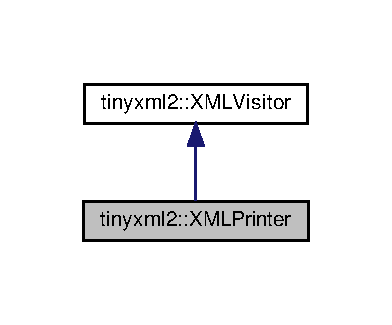
\includegraphics[width=188pt]{classtinyxml2_1_1_x_m_l_printer__inherit__graph}
\end{center}
\end{figure}


Collaboration diagram for tinyxml2\+:\+:X\+M\+L\+Printer\+:
\nopagebreak
\begin{figure}[H]
\begin{center}
\leavevmode
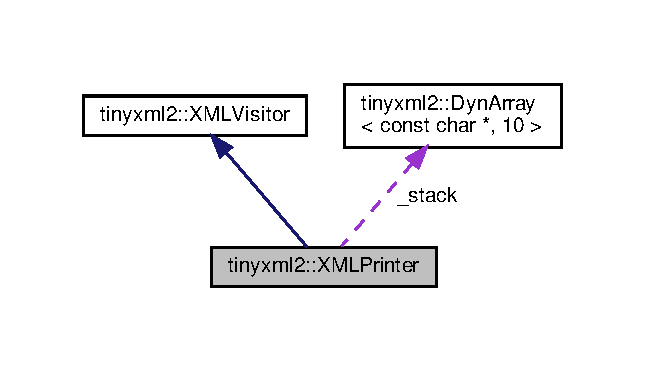
\includegraphics[width=310pt]{classtinyxml2_1_1_x_m_l_printer__coll__graph}
\end{center}
\end{figure}
\subsection*{Public Member Functions}
\begin{DoxyCompactItemize}
\item 
\hyperlink{classtinyxml2_1_1_x_m_l_printer_aa6d3841c069085f5b8a27bc7103c04f7}{X\+M\+L\+Printer} (F\+I\+LE $\ast$file=0, bool compact=false, int depth=0)
\item 
void \hyperlink{classtinyxml2_1_1_x_m_l_printer_a178c608ce8476043d5d6513819cde903}{Push\+Header} (bool write\+B\+OM, bool write\+Declaration)
\item 
void \hyperlink{classtinyxml2_1_1_x_m_l_printer_a20fb06c83bd13e5140d7dd13af06c010}{Open\+Element} (const char $\ast$name, bool compact\+Mode=false)
\item 
\mbox{\Hypertarget{classtinyxml2_1_1_x_m_l_printer_a9a4e2c9348b42e147629d5a99f4af3f0}\label{classtinyxml2_1_1_x_m_l_printer_a9a4e2c9348b42e147629d5a99f4af3f0}} 
void \hyperlink{classtinyxml2_1_1_x_m_l_printer_a9a4e2c9348b42e147629d5a99f4af3f0}{Push\+Attribute} (const char $\ast$name, const char $\ast$value)
\begin{DoxyCompactList}\small\item\em If streaming, add an attribute to an open element. \end{DoxyCompactList}\item 
\mbox{\Hypertarget{classtinyxml2_1_1_x_m_l_printer_a69120c82088597372d28d0a98f2ee7a1}\label{classtinyxml2_1_1_x_m_l_printer_a69120c82088597372d28d0a98f2ee7a1}} 
void {\bfseries Push\+Attribute} (const char $\ast$name, int value)
\item 
\mbox{\Hypertarget{classtinyxml2_1_1_x_m_l_printer_aa41039e51990aaf5342f3e0575a692c4}\label{classtinyxml2_1_1_x_m_l_printer_aa41039e51990aaf5342f3e0575a692c4}} 
void {\bfseries Push\+Attribute} (const char $\ast$name, unsigned value)
\item 
\mbox{\Hypertarget{classtinyxml2_1_1_x_m_l_printer_a9bc2fe21a83a70e6aa0415f2034ecbff}\label{classtinyxml2_1_1_x_m_l_printer_a9bc2fe21a83a70e6aa0415f2034ecbff}} 
void {\bfseries Push\+Attribute} (const char $\ast$name, int64\+\_\+t value)
\item 
\mbox{\Hypertarget{classtinyxml2_1_1_x_m_l_printer_a0cfb03811df0873faa59a12de009bf33}\label{classtinyxml2_1_1_x_m_l_printer_a0cfb03811df0873faa59a12de009bf33}} 
void {\bfseries Push\+Attribute} (const char $\ast$name, uint64\+\_\+t value)
\item 
\mbox{\Hypertarget{classtinyxml2_1_1_x_m_l_printer_a51f7950d7b7a19f0d3a0d549a318d45f}\label{classtinyxml2_1_1_x_m_l_printer_a51f7950d7b7a19f0d3a0d549a318d45f}} 
void {\bfseries Push\+Attribute} (const char $\ast$name, bool value)
\item 
\mbox{\Hypertarget{classtinyxml2_1_1_x_m_l_printer_a1714867af40e68ca404c3e84b6cac2a6}\label{classtinyxml2_1_1_x_m_l_printer_a1714867af40e68ca404c3e84b6cac2a6}} 
void {\bfseries Push\+Attribute} (const char $\ast$name, double value)
\item 
\mbox{\Hypertarget{classtinyxml2_1_1_x_m_l_printer_af1fb439e5d800999646f333fa2f0699a}\label{classtinyxml2_1_1_x_m_l_printer_af1fb439e5d800999646f333fa2f0699a}} 
virtual void \hyperlink{classtinyxml2_1_1_x_m_l_printer_af1fb439e5d800999646f333fa2f0699a}{Close\+Element} (bool compact\+Mode=false)
\begin{DoxyCompactList}\small\item\em If streaming, close the Element. \end{DoxyCompactList}\item 
\mbox{\Hypertarget{classtinyxml2_1_1_x_m_l_printer_a1cc16a9362df4332012cb13cff6441b3}\label{classtinyxml2_1_1_x_m_l_printer_a1cc16a9362df4332012cb13cff6441b3}} 
void \hyperlink{classtinyxml2_1_1_x_m_l_printer_a1cc16a9362df4332012cb13cff6441b3}{Push\+Text} (const char $\ast$text, bool cdata=false)
\begin{DoxyCompactList}\small\item\em Add a text node. \end{DoxyCompactList}\item 
\mbox{\Hypertarget{classtinyxml2_1_1_x_m_l_printer_a3e0d4d78de25d4cf081009e1431cea7e}\label{classtinyxml2_1_1_x_m_l_printer_a3e0d4d78de25d4cf081009e1431cea7e}} 
void \hyperlink{classtinyxml2_1_1_x_m_l_printer_a3e0d4d78de25d4cf081009e1431cea7e}{Push\+Text} (int value)
\begin{DoxyCompactList}\small\item\em Add a text node from an integer. \end{DoxyCompactList}\item 
\mbox{\Hypertarget{classtinyxml2_1_1_x_m_l_printer_a661fb50e7e0a4918d2d259cb0fae647e}\label{classtinyxml2_1_1_x_m_l_printer_a661fb50e7e0a4918d2d259cb0fae647e}} 
void \hyperlink{classtinyxml2_1_1_x_m_l_printer_a661fb50e7e0a4918d2d259cb0fae647e}{Push\+Text} (unsigned value)
\begin{DoxyCompactList}\small\item\em Add a text node from an unsigned. \end{DoxyCompactList}\item 
\mbox{\Hypertarget{classtinyxml2_1_1_x_m_l_printer_a96b0a0bfe105154a0a6c37d725258f0a}\label{classtinyxml2_1_1_x_m_l_printer_a96b0a0bfe105154a0a6c37d725258f0a}} 
void \hyperlink{classtinyxml2_1_1_x_m_l_printer_a96b0a0bfe105154a0a6c37d725258f0a}{Push\+Text} (int64\+\_\+t value)
\begin{DoxyCompactList}\small\item\em Add a text node from a signed 64bit integer. \end{DoxyCompactList}\item 
\mbox{\Hypertarget{classtinyxml2_1_1_x_m_l_printer_a60b0a4cf57371ff8679c2c7556ccb708}\label{classtinyxml2_1_1_x_m_l_printer_a60b0a4cf57371ff8679c2c7556ccb708}} 
void \hyperlink{classtinyxml2_1_1_x_m_l_printer_a60b0a4cf57371ff8679c2c7556ccb708}{Push\+Text} (uint64\+\_\+t value)
\begin{DoxyCompactList}\small\item\em Add a text node from an unsigned 64bit integer. \end{DoxyCompactList}\item 
\mbox{\Hypertarget{classtinyxml2_1_1_x_m_l_printer_a4390e5fa1ed05189a8686647345ab29f}\label{classtinyxml2_1_1_x_m_l_printer_a4390e5fa1ed05189a8686647345ab29f}} 
void \hyperlink{classtinyxml2_1_1_x_m_l_printer_a4390e5fa1ed05189a8686647345ab29f}{Push\+Text} (bool value)
\begin{DoxyCompactList}\small\item\em Add a text node from a bool. \end{DoxyCompactList}\item 
\mbox{\Hypertarget{classtinyxml2_1_1_x_m_l_printer_a1dbb1390e829d0673af66b9cd1928bd7}\label{classtinyxml2_1_1_x_m_l_printer_a1dbb1390e829d0673af66b9cd1928bd7}} 
void \hyperlink{classtinyxml2_1_1_x_m_l_printer_a1dbb1390e829d0673af66b9cd1928bd7}{Push\+Text} (float value)
\begin{DoxyCompactList}\small\item\em Add a text node from a float. \end{DoxyCompactList}\item 
\mbox{\Hypertarget{classtinyxml2_1_1_x_m_l_printer_aa715302dfc09473c77c853cbd5431965}\label{classtinyxml2_1_1_x_m_l_printer_aa715302dfc09473c77c853cbd5431965}} 
void \hyperlink{classtinyxml2_1_1_x_m_l_printer_aa715302dfc09473c77c853cbd5431965}{Push\+Text} (double value)
\begin{DoxyCompactList}\small\item\em Add a text node from a double. \end{DoxyCompactList}\item 
\mbox{\Hypertarget{classtinyxml2_1_1_x_m_l_printer_afc8416814219591c2fd5656e0c233140}\label{classtinyxml2_1_1_x_m_l_printer_afc8416814219591c2fd5656e0c233140}} 
void \hyperlink{classtinyxml2_1_1_x_m_l_printer_afc8416814219591c2fd5656e0c233140}{Push\+Comment} (const char $\ast$comment)
\begin{DoxyCompactList}\small\item\em Add a comment. \end{DoxyCompactList}\item 
\mbox{\Hypertarget{classtinyxml2_1_1_x_m_l_printer_a2fe3565e262594efc6c0276723c83fe7}\label{classtinyxml2_1_1_x_m_l_printer_a2fe3565e262594efc6c0276723c83fe7}} 
void {\bfseries Push\+Declaration} (const char $\ast$value)
\item 
\mbox{\Hypertarget{classtinyxml2_1_1_x_m_l_printer_ab1efc6d1548505e9984185f58f54b713}\label{classtinyxml2_1_1_x_m_l_printer_ab1efc6d1548505e9984185f58f54b713}} 
void {\bfseries Push\+Unknown} (const char $\ast$value)
\item 
\mbox{\Hypertarget{classtinyxml2_1_1_x_m_l_printer_a9aa1de11a55a07db55a90fde37d7afad}\label{classtinyxml2_1_1_x_m_l_printer_a9aa1de11a55a07db55a90fde37d7afad}} 
virtual bool \hyperlink{classtinyxml2_1_1_x_m_l_printer_a9aa1de11a55a07db55a90fde37d7afad}{Visit\+Enter} (const \hyperlink{classtinyxml2_1_1_x_m_l_document}{X\+M\+L\+Document} \&)
\begin{DoxyCompactList}\small\item\em Visit a document. \end{DoxyCompactList}\item 
\mbox{\Hypertarget{classtinyxml2_1_1_x_m_l_printer_a15fc1f2b922f540917dcf52808737b29}\label{classtinyxml2_1_1_x_m_l_printer_a15fc1f2b922f540917dcf52808737b29}} 
virtual bool \hyperlink{classtinyxml2_1_1_x_m_l_printer_a15fc1f2b922f540917dcf52808737b29}{Visit\+Exit} (const \hyperlink{classtinyxml2_1_1_x_m_l_document}{X\+M\+L\+Document} \&)
\begin{DoxyCompactList}\small\item\em Visit a document. \end{DoxyCompactList}\item 
\mbox{\Hypertarget{classtinyxml2_1_1_x_m_l_printer_a169b2509d8eabb70811b2bb8cfd1f5d1}\label{classtinyxml2_1_1_x_m_l_printer_a169b2509d8eabb70811b2bb8cfd1f5d1}} 
virtual bool \hyperlink{classtinyxml2_1_1_x_m_l_printer_a169b2509d8eabb70811b2bb8cfd1f5d1}{Visit\+Enter} (const \hyperlink{classtinyxml2_1_1_x_m_l_element}{X\+M\+L\+Element} \&element, const \hyperlink{classtinyxml2_1_1_x_m_l_attribute}{X\+M\+L\+Attribute} $\ast$attribute)
\begin{DoxyCompactList}\small\item\em Visit an element. \end{DoxyCompactList}\item 
\mbox{\Hypertarget{classtinyxml2_1_1_x_m_l_printer_a2edd48405971a88951c71c9df86a2f50}\label{classtinyxml2_1_1_x_m_l_printer_a2edd48405971a88951c71c9df86a2f50}} 
virtual bool \hyperlink{classtinyxml2_1_1_x_m_l_printer_a2edd48405971a88951c71c9df86a2f50}{Visit\+Exit} (const \hyperlink{classtinyxml2_1_1_x_m_l_element}{X\+M\+L\+Element} \&element)
\begin{DoxyCompactList}\small\item\em Visit an element. \end{DoxyCompactList}\item 
\mbox{\Hypertarget{classtinyxml2_1_1_x_m_l_printer_adc0e42b4f6fcb90a95630c79575d030b}\label{classtinyxml2_1_1_x_m_l_printer_adc0e42b4f6fcb90a95630c79575d030b}} 
virtual bool \hyperlink{classtinyxml2_1_1_x_m_l_printer_adc0e42b4f6fcb90a95630c79575d030b}{Visit} (const \hyperlink{classtinyxml2_1_1_x_m_l_text}{X\+M\+L\+Text} \&text)
\begin{DoxyCompactList}\small\item\em Visit a text node. \end{DoxyCompactList}\item 
\mbox{\Hypertarget{classtinyxml2_1_1_x_m_l_printer_aa294c5c01af0ebb9114902456e4cb53c}\label{classtinyxml2_1_1_x_m_l_printer_aa294c5c01af0ebb9114902456e4cb53c}} 
virtual bool \hyperlink{classtinyxml2_1_1_x_m_l_printer_aa294c5c01af0ebb9114902456e4cb53c}{Visit} (const \hyperlink{classtinyxml2_1_1_x_m_l_comment}{X\+M\+L\+Comment} \&comment)
\begin{DoxyCompactList}\small\item\em Visit a comment node. \end{DoxyCompactList}\item 
\mbox{\Hypertarget{classtinyxml2_1_1_x_m_l_printer_acfc625b2549304b9c7eb85ebd5c5eb39}\label{classtinyxml2_1_1_x_m_l_printer_acfc625b2549304b9c7eb85ebd5c5eb39}} 
virtual bool \hyperlink{classtinyxml2_1_1_x_m_l_printer_acfc625b2549304b9c7eb85ebd5c5eb39}{Visit} (const \hyperlink{classtinyxml2_1_1_x_m_l_declaration}{X\+M\+L\+Declaration} \&declaration)
\begin{DoxyCompactList}\small\item\em Visit a declaration. \end{DoxyCompactList}\item 
\mbox{\Hypertarget{classtinyxml2_1_1_x_m_l_printer_ab8af5455bbf9e4be2663e6642fcd7e32}\label{classtinyxml2_1_1_x_m_l_printer_ab8af5455bbf9e4be2663e6642fcd7e32}} 
virtual bool \hyperlink{classtinyxml2_1_1_x_m_l_printer_ab8af5455bbf9e4be2663e6642fcd7e32}{Visit} (const \hyperlink{classtinyxml2_1_1_x_m_l_unknown}{X\+M\+L\+Unknown} \&unknown)
\begin{DoxyCompactList}\small\item\em Visit an unknown node. \end{DoxyCompactList}\item 
const char $\ast$ \hyperlink{classtinyxml2_1_1_x_m_l_printer_a180671d73844f159f2d4aafbc11d106e}{C\+Str} () const
\item 
int \hyperlink{classtinyxml2_1_1_x_m_l_printer_a3256cf3523d4898b91abb18b924be04c}{C\+Str\+Size} () const
\item 
void \hyperlink{classtinyxml2_1_1_x_m_l_printer_a690cb140ba98b7339734ff865f56b0b3}{Clear\+Buffer} (bool reset\+To\+First\+Element=true)
\end{DoxyCompactItemize}
\subsection*{Protected Member Functions}
\begin{DoxyCompactItemize}
\item 
\mbox{\Hypertarget{classtinyxml2_1_1_x_m_l_printer_a38e1ed5a779bdf63eda9e808f7a6de66}\label{classtinyxml2_1_1_x_m_l_printer_a38e1ed5a779bdf63eda9e808f7a6de66}} 
virtual bool {\bfseries Compact\+Mode} (const \hyperlink{classtinyxml2_1_1_x_m_l_element}{X\+M\+L\+Element} \&)
\item 
virtual void \hyperlink{classtinyxml2_1_1_x_m_l_printer_a1c4b2ccbe4fdb316d54f5a93f3559260}{Print\+Space} (int depth)
\item 
\mbox{\Hypertarget{classtinyxml2_1_1_x_m_l_printer_ab30210a7f32e45634e7a45137bf6fdf6}\label{classtinyxml2_1_1_x_m_l_printer_ab30210a7f32e45634e7a45137bf6fdf6}} 
void {\bfseries Print} (const char $\ast$format,...)
\item 
\mbox{\Hypertarget{classtinyxml2_1_1_x_m_l_printer_aff363b7634a27538fd691ae62adbda63}\label{classtinyxml2_1_1_x_m_l_printer_aff363b7634a27538fd691ae62adbda63}} 
void {\bfseries Write} (const char $\ast$data, size\+\_\+t size)
\item 
\mbox{\Hypertarget{classtinyxml2_1_1_x_m_l_printer_a4bd7f0cabca77ac95c299103fa9592f1}\label{classtinyxml2_1_1_x_m_l_printer_a4bd7f0cabca77ac95c299103fa9592f1}} 
void {\bfseries Write} (const char $\ast$data)
\item 
\mbox{\Hypertarget{classtinyxml2_1_1_x_m_l_printer_a9567b0218169ba59794f171ae2f9944c}\label{classtinyxml2_1_1_x_m_l_printer_a9567b0218169ba59794f171ae2f9944c}} 
void {\bfseries Putc} (char ch)
\item 
\mbox{\Hypertarget{classtinyxml2_1_1_x_m_l_printer_ac6e2c72c5d796f5b4de6ce81ca95e3fa}\label{classtinyxml2_1_1_x_m_l_printer_ac6e2c72c5d796f5b4de6ce81ca95e3fa}} 
void {\bfseries Seal\+Element\+If\+Just\+Opened} ()
\end{DoxyCompactItemize}
\subsection*{Protected Attributes}
\begin{DoxyCompactItemize}
\item 
\mbox{\Hypertarget{classtinyxml2_1_1_x_m_l_printer_ac07169d58b465214a2b1fa306e617c26}\label{classtinyxml2_1_1_x_m_l_printer_ac07169d58b465214a2b1fa306e617c26}} 
bool {\bfseries \+\_\+element\+Just\+Opened}
\item 
\mbox{\Hypertarget{classtinyxml2_1_1_x_m_l_printer_a99d59e67e084714541bee3ae43884bef}\label{classtinyxml2_1_1_x_m_l_printer_a99d59e67e084714541bee3ae43884bef}} 
\hyperlink{classtinyxml2_1_1_dyn_array}{Dyn\+Array}$<$ const char $\ast$, 10 $>$ {\bfseries \+\_\+stack}
\end{DoxyCompactItemize}


\subsection{Detailed Description}
Printing functionality. The \hyperlink{classtinyxml2_1_1_x_m_l_printer}{X\+M\+L\+Printer} gives you more options than the \hyperlink{classtinyxml2_1_1_x_m_l_document_a867cf5fa3e3ff6ae4847a8b7ee8ec083}{X\+M\+L\+Document\+::\+Print()} method.

It can\+:
\begin{DoxyEnumerate}
\item Print to memory.
\item Print to a file you provide.
\item Print X\+ML without a \hyperlink{classtinyxml2_1_1_x_m_l_document}{X\+M\+L\+Document}.
\end{DoxyEnumerate}

Print to Memory

\begin{DoxyVerb}XMLPrinter printer;
doc.Print( &printer );
SomeFunction( printer.CStr() );
\end{DoxyVerb}


Print to a File

You provide the file pointer. \begin{DoxyVerb}XMLPrinter printer( fp );
doc.Print( &printer );
\end{DoxyVerb}


Print without a \hyperlink{classtinyxml2_1_1_x_m_l_document}{X\+M\+L\+Document}

When loading, an X\+ML parser is very useful. However, sometimes when saving, it just gets in the way. The code is often set up for streaming, and constructing the D\+OM is just overhead.

The Printer supports the streaming case. The following code prints out a trivially simple X\+ML file without ever creating an X\+ML document.

\begin{DoxyVerb}XMLPrinter printer( fp );
printer.OpenElement( "foo" );
printer.PushAttribute( "foo", "bar" );
printer.CloseElement();
\end{DoxyVerb}
 

\subsection{Constructor \& Destructor Documentation}
\mbox{\Hypertarget{classtinyxml2_1_1_x_m_l_printer_aa6d3841c069085f5b8a27bc7103c04f7}\label{classtinyxml2_1_1_x_m_l_printer_aa6d3841c069085f5b8a27bc7103c04f7}} 
\index{tinyxml2\+::\+X\+M\+L\+Printer@{tinyxml2\+::\+X\+M\+L\+Printer}!X\+M\+L\+Printer@{X\+M\+L\+Printer}}
\index{X\+M\+L\+Printer@{X\+M\+L\+Printer}!tinyxml2\+::\+X\+M\+L\+Printer@{tinyxml2\+::\+X\+M\+L\+Printer}}
\subsubsection{\texorpdfstring{X\+M\+L\+Printer()}{XMLPrinter()}}
{\footnotesize\ttfamily tinyxml2\+::\+X\+M\+L\+Printer\+::\+X\+M\+L\+Printer (\begin{DoxyParamCaption}\item[{F\+I\+LE $\ast$}]{file = {\ttfamily 0},  }\item[{bool}]{compact = {\ttfamily false},  }\item[{int}]{depth = {\ttfamily 0} }\end{DoxyParamCaption})}

Construct the printer. If the F\+I\+L\+E$\ast$ is specified, this will print to the F\+I\+LE. Else it will print to memory, and the result is available in \hyperlink{classtinyxml2_1_1_x_m_l_printer_a180671d73844f159f2d4aafbc11d106e}{C\+Str()}. If \textquotesingle{}compact\textquotesingle{} is set to true, then output is created with only required whitespace and newlines. 

\subsection{Member Function Documentation}
\mbox{\Hypertarget{classtinyxml2_1_1_x_m_l_printer_a690cb140ba98b7339734ff865f56b0b3}\label{classtinyxml2_1_1_x_m_l_printer_a690cb140ba98b7339734ff865f56b0b3}} 
\index{tinyxml2\+::\+X\+M\+L\+Printer@{tinyxml2\+::\+X\+M\+L\+Printer}!Clear\+Buffer@{Clear\+Buffer}}
\index{Clear\+Buffer@{Clear\+Buffer}!tinyxml2\+::\+X\+M\+L\+Printer@{tinyxml2\+::\+X\+M\+L\+Printer}}
\subsubsection{\texorpdfstring{Clear\+Buffer()}{ClearBuffer()}}
{\footnotesize\ttfamily void tinyxml2\+::\+X\+M\+L\+Printer\+::\+Clear\+Buffer (\begin{DoxyParamCaption}\item[{bool}]{reset\+To\+First\+Element = {\ttfamily true} }\end{DoxyParamCaption})\hspace{0.3cm}{\ttfamily [inline]}}

If in print to memory mode, reset the buffer to the beginning. \mbox{\Hypertarget{classtinyxml2_1_1_x_m_l_printer_a180671d73844f159f2d4aafbc11d106e}\label{classtinyxml2_1_1_x_m_l_printer_a180671d73844f159f2d4aafbc11d106e}} 
\index{tinyxml2\+::\+X\+M\+L\+Printer@{tinyxml2\+::\+X\+M\+L\+Printer}!C\+Str@{C\+Str}}
\index{C\+Str@{C\+Str}!tinyxml2\+::\+X\+M\+L\+Printer@{tinyxml2\+::\+X\+M\+L\+Printer}}
\subsubsection{\texorpdfstring{C\+Str()}{CStr()}}
{\footnotesize\ttfamily const char$\ast$ tinyxml2\+::\+X\+M\+L\+Printer\+::\+C\+Str (\begin{DoxyParamCaption}{ }\end{DoxyParamCaption}) const\hspace{0.3cm}{\ttfamily [inline]}}

If in print to memory mode, return a pointer to the X\+ML file in memory. \mbox{\Hypertarget{classtinyxml2_1_1_x_m_l_printer_a3256cf3523d4898b91abb18b924be04c}\label{classtinyxml2_1_1_x_m_l_printer_a3256cf3523d4898b91abb18b924be04c}} 
\index{tinyxml2\+::\+X\+M\+L\+Printer@{tinyxml2\+::\+X\+M\+L\+Printer}!C\+Str\+Size@{C\+Str\+Size}}
\index{C\+Str\+Size@{C\+Str\+Size}!tinyxml2\+::\+X\+M\+L\+Printer@{tinyxml2\+::\+X\+M\+L\+Printer}}
\subsubsection{\texorpdfstring{C\+Str\+Size()}{CStrSize()}}
{\footnotesize\ttfamily int tinyxml2\+::\+X\+M\+L\+Printer\+::\+C\+Str\+Size (\begin{DoxyParamCaption}{ }\end{DoxyParamCaption}) const\hspace{0.3cm}{\ttfamily [inline]}}

If in print to memory mode, return the size of the X\+ML file in memory. (Note the size returned includes the terminating null.) \mbox{\Hypertarget{classtinyxml2_1_1_x_m_l_printer_a20fb06c83bd13e5140d7dd13af06c010}\label{classtinyxml2_1_1_x_m_l_printer_a20fb06c83bd13e5140d7dd13af06c010}} 
\index{tinyxml2\+::\+X\+M\+L\+Printer@{tinyxml2\+::\+X\+M\+L\+Printer}!Open\+Element@{Open\+Element}}
\index{Open\+Element@{Open\+Element}!tinyxml2\+::\+X\+M\+L\+Printer@{tinyxml2\+::\+X\+M\+L\+Printer}}
\subsubsection{\texorpdfstring{Open\+Element()}{OpenElement()}}
{\footnotesize\ttfamily void tinyxml2\+::\+X\+M\+L\+Printer\+::\+Open\+Element (\begin{DoxyParamCaption}\item[{const char $\ast$}]{name,  }\item[{bool}]{compact\+Mode = {\ttfamily false} }\end{DoxyParamCaption})}

If streaming, start writing an element. The element must be closed with \hyperlink{classtinyxml2_1_1_x_m_l_printer_af1fb439e5d800999646f333fa2f0699a}{Close\+Element()} \mbox{\Hypertarget{classtinyxml2_1_1_x_m_l_printer_a1c4b2ccbe4fdb316d54f5a93f3559260}\label{classtinyxml2_1_1_x_m_l_printer_a1c4b2ccbe4fdb316d54f5a93f3559260}} 
\index{tinyxml2\+::\+X\+M\+L\+Printer@{tinyxml2\+::\+X\+M\+L\+Printer}!Print\+Space@{Print\+Space}}
\index{Print\+Space@{Print\+Space}!tinyxml2\+::\+X\+M\+L\+Printer@{tinyxml2\+::\+X\+M\+L\+Printer}}
\subsubsection{\texorpdfstring{Print\+Space()}{PrintSpace()}}
{\footnotesize\ttfamily void tinyxml2\+::\+X\+M\+L\+Printer\+::\+Print\+Space (\begin{DoxyParamCaption}\item[{int}]{depth }\end{DoxyParamCaption})\hspace{0.3cm}{\ttfamily [protected]}, {\ttfamily [virtual]}}

Prints out the space before an element. You may override to change the space and tabs used. A \hyperlink{classtinyxml2_1_1_x_m_l_printer_a1c4b2ccbe4fdb316d54f5a93f3559260}{Print\+Space()} override should call Print(). \mbox{\Hypertarget{classtinyxml2_1_1_x_m_l_printer_a178c608ce8476043d5d6513819cde903}\label{classtinyxml2_1_1_x_m_l_printer_a178c608ce8476043d5d6513819cde903}} 
\index{tinyxml2\+::\+X\+M\+L\+Printer@{tinyxml2\+::\+X\+M\+L\+Printer}!Push\+Header@{Push\+Header}}
\index{Push\+Header@{Push\+Header}!tinyxml2\+::\+X\+M\+L\+Printer@{tinyxml2\+::\+X\+M\+L\+Printer}}
\subsubsection{\texorpdfstring{Push\+Header()}{PushHeader()}}
{\footnotesize\ttfamily void tinyxml2\+::\+X\+M\+L\+Printer\+::\+Push\+Header (\begin{DoxyParamCaption}\item[{bool}]{write\+B\+OM,  }\item[{bool}]{write\+Declaration }\end{DoxyParamCaption})}

If streaming, write the B\+OM and declaration. 

The documentation for this class was generated from the following files\+:\begin{DoxyCompactItemize}
\item 
/home/ijlee/workspace/sdmt/src/tinyxml2.\+h\item 
/home/ijlee/workspace/sdmt/src/tinyxml2.\+cpp\end{DoxyCompactItemize}

\hypertarget{classtinyxml2_1_1_x_m_l_text}{}\section{tinyxml2\+:\+:X\+M\+L\+Text Class Reference}
\label{classtinyxml2_1_1_x_m_l_text}\index{tinyxml2\+::\+X\+M\+L\+Text@{tinyxml2\+::\+X\+M\+L\+Text}}


{\ttfamily \#include $<$tinyxml2.\+h$>$}



Inheritance diagram for tinyxml2\+:\+:X\+M\+L\+Text\+:
\nopagebreak
\begin{figure}[H]
\begin{center}
\leavevmode
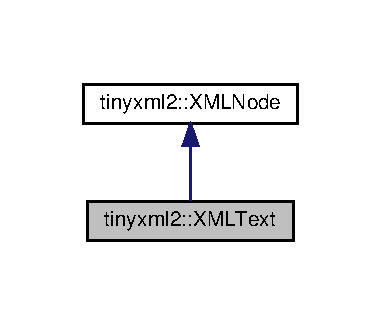
\includegraphics[width=183pt]{classtinyxml2_1_1_x_m_l_text__inherit__graph}
\end{center}
\end{figure}


Collaboration diagram for tinyxml2\+:\+:X\+M\+L\+Text\+:
\nopagebreak
\begin{figure}[H]
\begin{center}
\leavevmode
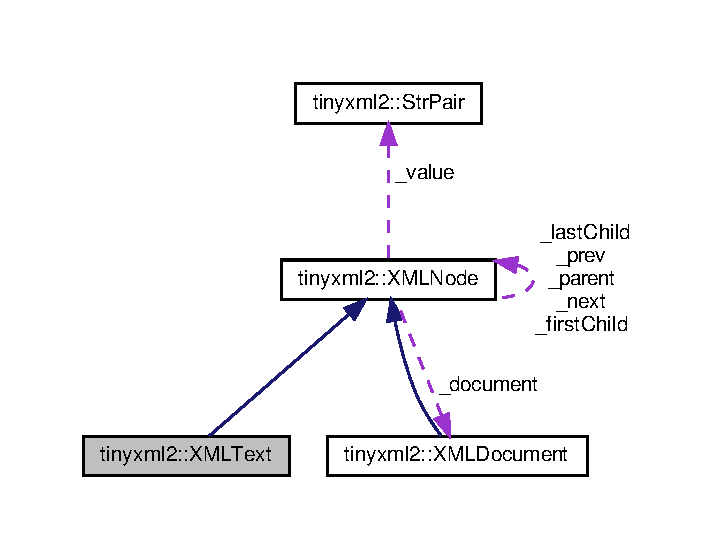
\includegraphics[width=343pt]{classtinyxml2_1_1_x_m_l_text__coll__graph}
\end{center}
\end{figure}
\subsection*{Public Member Functions}
\begin{DoxyCompactItemize}
\item 
virtual bool \hyperlink{classtinyxml2_1_1_x_m_l_text_a537c60d7e18fb59c45ac2737a29ac47a}{Accept} (\hyperlink{classtinyxml2_1_1_x_m_l_visitor}{X\+M\+L\+Visitor} $\ast$visitor) const
\item 
\mbox{\Hypertarget{classtinyxml2_1_1_x_m_l_text_ab1213b4ddebe9b17ec7e7040e9f1caf7}\label{classtinyxml2_1_1_x_m_l_text_ab1213b4ddebe9b17ec7e7040e9f1caf7}} 
virtual \hyperlink{classtinyxml2_1_1_x_m_l_text}{X\+M\+L\+Text} $\ast$ \hyperlink{classtinyxml2_1_1_x_m_l_text_ab1213b4ddebe9b17ec7e7040e9f1caf7}{To\+Text} ()
\begin{DoxyCompactList}\small\item\em Safely cast to Text, or null. \end{DoxyCompactList}\item 
\mbox{\Hypertarget{classtinyxml2_1_1_x_m_l_text_a671ce22c7c5ef378f1ce31e6f827b9e2}\label{classtinyxml2_1_1_x_m_l_text_a671ce22c7c5ef378f1ce31e6f827b9e2}} 
virtual const \hyperlink{classtinyxml2_1_1_x_m_l_text}{X\+M\+L\+Text} $\ast$ {\bfseries To\+Text} () const
\item 
\mbox{\Hypertarget{classtinyxml2_1_1_x_m_l_text_ad080357d76ab7cc59d7651249949329d}\label{classtinyxml2_1_1_x_m_l_text_ad080357d76ab7cc59d7651249949329d}} 
void \hyperlink{classtinyxml2_1_1_x_m_l_text_ad080357d76ab7cc59d7651249949329d}{Set\+C\+Data} (bool is\+C\+Data)
\begin{DoxyCompactList}\small\item\em Declare whether this should be C\+D\+A\+TA or standard text. \end{DoxyCompactList}\item 
\mbox{\Hypertarget{classtinyxml2_1_1_x_m_l_text_ac1bb5ea4166c320882d9e0ad16fd385b}\label{classtinyxml2_1_1_x_m_l_text_ac1bb5ea4166c320882d9e0ad16fd385b}} 
bool \hyperlink{classtinyxml2_1_1_x_m_l_text_ac1bb5ea4166c320882d9e0ad16fd385b}{C\+Data} () const
\begin{DoxyCompactList}\small\item\em Returns true if this is a C\+D\+A\+TA text element. \end{DoxyCompactList}\item 
virtual \hyperlink{classtinyxml2_1_1_x_m_l_node}{X\+M\+L\+Node} $\ast$ \hyperlink{classtinyxml2_1_1_x_m_l_text_a86d265c93152726c8c6831e9594840e6}{Shallow\+Clone} (\hyperlink{classtinyxml2_1_1_x_m_l_document}{X\+M\+L\+Document} $\ast$document) const
\item 
virtual bool \hyperlink{classtinyxml2_1_1_x_m_l_text_a99d8bce4dc01df889126e047f358cdfc}{Shallow\+Equal} (const \hyperlink{classtinyxml2_1_1_x_m_l_node}{X\+M\+L\+Node} $\ast$compare) const
\end{DoxyCompactItemize}
\subsection*{Protected Member Functions}
\begin{DoxyCompactItemize}
\item 
\mbox{\Hypertarget{classtinyxml2_1_1_x_m_l_text_ad9f46d70e61e5386ead93728d8b90267}\label{classtinyxml2_1_1_x_m_l_text_ad9f46d70e61e5386ead93728d8b90267}} 
{\bfseries X\+M\+L\+Text} (\hyperlink{classtinyxml2_1_1_x_m_l_document}{X\+M\+L\+Document} $\ast$doc)
\item 
\mbox{\Hypertarget{classtinyxml2_1_1_x_m_l_text_af3b93344f1183482e1683f5922ac9c68}\label{classtinyxml2_1_1_x_m_l_text_af3b93344f1183482e1683f5922ac9c68}} 
char $\ast$ {\bfseries Parse\+Deep} (char $\ast$p, \hyperlink{classtinyxml2_1_1_str_pair}{Str\+Pair} $\ast$parent\+End\+Tag, int $\ast$cur\+Line\+Num\+Ptr)
\end{DoxyCompactItemize}
\subsection*{Friends}
\begin{DoxyCompactItemize}
\item 
\mbox{\Hypertarget{classtinyxml2_1_1_x_m_l_text_a4eee3bda60c60a30e4e8cd4ea91c4c6e}\label{classtinyxml2_1_1_x_m_l_text_a4eee3bda60c60a30e4e8cd4ea91c4c6e}} 
class {\bfseries X\+M\+L\+Document}
\end{DoxyCompactItemize}
\subsection*{Additional Inherited Members}


\subsection{Detailed Description}
X\+ML text.

Note that a text node can have child element nodes, for example\+: \begin{DoxyVerb}<root>This is <b>bold</b></root>
\end{DoxyVerb}


A text node can have 2 ways to output the next. \char`\"{}normal\char`\"{} output and C\+D\+A\+TA. It will default to the mode it was parsed from the X\+ML file and you generally want to leave it alone, but you can change the output mode with \hyperlink{classtinyxml2_1_1_x_m_l_text_ad080357d76ab7cc59d7651249949329d}{Set\+C\+Data()} and query it with \hyperlink{classtinyxml2_1_1_x_m_l_text_ac1bb5ea4166c320882d9e0ad16fd385b}{C\+Data()}. 

\subsection{Member Function Documentation}
\mbox{\Hypertarget{classtinyxml2_1_1_x_m_l_text_a537c60d7e18fb59c45ac2737a29ac47a}\label{classtinyxml2_1_1_x_m_l_text_a537c60d7e18fb59c45ac2737a29ac47a}} 
\index{tinyxml2\+::\+X\+M\+L\+Text@{tinyxml2\+::\+X\+M\+L\+Text}!Accept@{Accept}}
\index{Accept@{Accept}!tinyxml2\+::\+X\+M\+L\+Text@{tinyxml2\+::\+X\+M\+L\+Text}}
\subsubsection{\texorpdfstring{Accept()}{Accept()}}
{\footnotesize\ttfamily bool tinyxml2\+::\+X\+M\+L\+Text\+::\+Accept (\begin{DoxyParamCaption}\item[{\hyperlink{classtinyxml2_1_1_x_m_l_visitor}{X\+M\+L\+Visitor} $\ast$}]{visitor }\end{DoxyParamCaption}) const\hspace{0.3cm}{\ttfamily [virtual]}}

Accept a hierarchical visit of the nodes in the Tiny\+X\+M\+L-\/2 D\+OM. Every node in the X\+ML tree will be conditionally visited and the host will be called back via the \hyperlink{classtinyxml2_1_1_x_m_l_visitor}{X\+M\+L\+Visitor} interface.

This is essentially a S\+AX interface for Tiny\+X\+M\+L-\/2. (Note however it doesn\textquotesingle{}t re-\/parse the X\+ML for the callbacks, so the performance of Tiny\+X\+M\+L-\/2 is unchanged by using this interface versus any other.)

The interface has been based on ideas from\+:


\begin{DoxyItemize}
\item \href{http://www.saxproject.org/}{\tt http\+://www.\+saxproject.\+org/}
\item \href{http://c2.com/cgi/wiki?HierarchicalVisitorPattern}{\tt http\+://c2.\+com/cgi/wiki?\+Hierarchical\+Visitor\+Pattern}
\end{DoxyItemize}

Which are both good references for \char`\"{}visiting\char`\"{}.

An example of using \hyperlink{classtinyxml2_1_1_x_m_l_text_a537c60d7e18fb59c45ac2737a29ac47a}{Accept()}\+: \begin{DoxyVerb}XMLPrinter printer;
tinyxmlDoc.Accept( &printer );
const char* xmlcstr = printer.CStr();
\end{DoxyVerb}
 

Implements \hyperlink{classtinyxml2_1_1_x_m_l_node_a81e66df0a44c67a7af17f3b77a152785}{tinyxml2\+::\+X\+M\+L\+Node}.

\mbox{\Hypertarget{classtinyxml2_1_1_x_m_l_text_a86d265c93152726c8c6831e9594840e6}\label{classtinyxml2_1_1_x_m_l_text_a86d265c93152726c8c6831e9594840e6}} 
\index{tinyxml2\+::\+X\+M\+L\+Text@{tinyxml2\+::\+X\+M\+L\+Text}!Shallow\+Clone@{Shallow\+Clone}}
\index{Shallow\+Clone@{Shallow\+Clone}!tinyxml2\+::\+X\+M\+L\+Text@{tinyxml2\+::\+X\+M\+L\+Text}}
\subsubsection{\texorpdfstring{Shallow\+Clone()}{ShallowClone()}}
{\footnotesize\ttfamily \hyperlink{classtinyxml2_1_1_x_m_l_node}{X\+M\+L\+Node} $\ast$ tinyxml2\+::\+X\+M\+L\+Text\+::\+Shallow\+Clone (\begin{DoxyParamCaption}\item[{\hyperlink{classtinyxml2_1_1_x_m_l_document}{X\+M\+L\+Document} $\ast$}]{document }\end{DoxyParamCaption}) const\hspace{0.3cm}{\ttfamily [virtual]}}

Make a copy of this node, but not its children. You may pass in a Document pointer that will be the owner of the new Node. If the \textquotesingle{}document\textquotesingle{} is null, then the node returned will be allocated from the current Document. (this-\/$>$\hyperlink{classtinyxml2_1_1_x_m_l_node_af343d1ef0b45c0020e62d784d7e67a68}{Get\+Document()})

Note\+: if called on a \hyperlink{classtinyxml2_1_1_x_m_l_document}{X\+M\+L\+Document}, this will return null. 

Implements \hyperlink{classtinyxml2_1_1_x_m_l_node_a8402cbd3129d20e9e6024bbcc0531283}{tinyxml2\+::\+X\+M\+L\+Node}.

\mbox{\Hypertarget{classtinyxml2_1_1_x_m_l_text_a99d8bce4dc01df889126e047f358cdfc}\label{classtinyxml2_1_1_x_m_l_text_a99d8bce4dc01df889126e047f358cdfc}} 
\index{tinyxml2\+::\+X\+M\+L\+Text@{tinyxml2\+::\+X\+M\+L\+Text}!Shallow\+Equal@{Shallow\+Equal}}
\index{Shallow\+Equal@{Shallow\+Equal}!tinyxml2\+::\+X\+M\+L\+Text@{tinyxml2\+::\+X\+M\+L\+Text}}
\subsubsection{\texorpdfstring{Shallow\+Equal()}{ShallowEqual()}}
{\footnotesize\ttfamily bool tinyxml2\+::\+X\+M\+L\+Text\+::\+Shallow\+Equal (\begin{DoxyParamCaption}\item[{const \hyperlink{classtinyxml2_1_1_x_m_l_node}{X\+M\+L\+Node} $\ast$}]{compare }\end{DoxyParamCaption}) const\hspace{0.3cm}{\ttfamily [virtual]}}

Test if 2 nodes are the same, but don\textquotesingle{}t test children. The 2 nodes do not need to be in the same Document.

Note\+: if called on a \hyperlink{classtinyxml2_1_1_x_m_l_document}{X\+M\+L\+Document}, this will return false. 

Implements \hyperlink{classtinyxml2_1_1_x_m_l_node_a7ce18b751c3ea09eac292dca264f9226}{tinyxml2\+::\+X\+M\+L\+Node}.



The documentation for this class was generated from the following files\+:\begin{DoxyCompactItemize}
\item 
/home/ijlee/workspace/sdmt/src/tinyxml2.\+h\item 
/home/ijlee/workspace/sdmt/src/tinyxml2.\+cpp\end{DoxyCompactItemize}

\hypertarget{classtinyxml2_1_1_x_m_l_unknown}{}\section{tinyxml2\+:\+:X\+M\+L\+Unknown Class Reference}
\label{classtinyxml2_1_1_x_m_l_unknown}\index{tinyxml2\+::\+X\+M\+L\+Unknown@{tinyxml2\+::\+X\+M\+L\+Unknown}}


{\ttfamily \#include $<$tinyxml2.\+h$>$}



Inheritance diagram for tinyxml2\+:\+:X\+M\+L\+Unknown\+:
\nopagebreak
\begin{figure}[H]
\begin{center}
\leavevmode
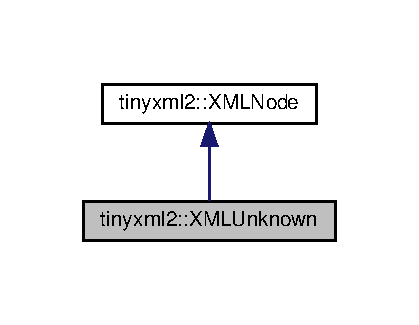
\includegraphics[width=201pt]{classtinyxml2_1_1_x_m_l_unknown__inherit__graph}
\end{center}
\end{figure}


Collaboration diagram for tinyxml2\+:\+:X\+M\+L\+Unknown\+:
\nopagebreak
\begin{figure}[H]
\begin{center}
\leavevmode
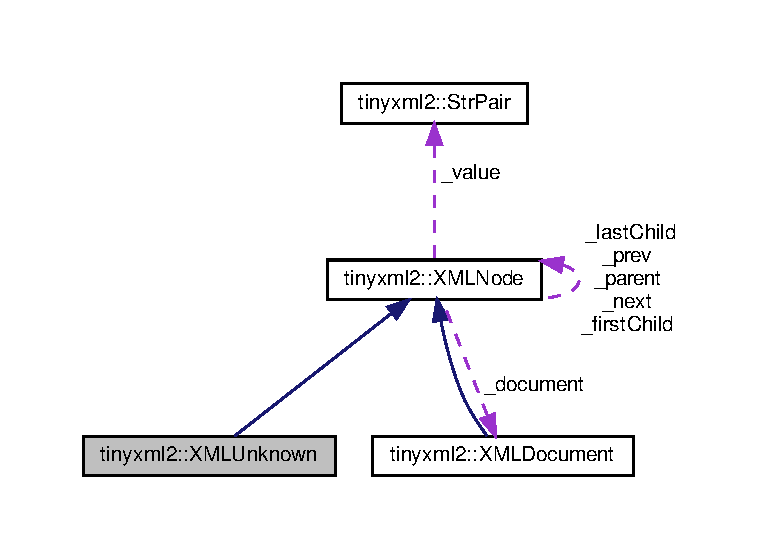
\includegraphics[width=350pt]{classtinyxml2_1_1_x_m_l_unknown__coll__graph}
\end{center}
\end{figure}
\subsection*{Public Member Functions}
\begin{DoxyCompactItemize}
\item 
\mbox{\Hypertarget{classtinyxml2_1_1_x_m_l_unknown_af4374856421921cad578c8affae872b6}\label{classtinyxml2_1_1_x_m_l_unknown_af4374856421921cad578c8affae872b6}} 
virtual \hyperlink{classtinyxml2_1_1_x_m_l_unknown}{X\+M\+L\+Unknown} $\ast$ \hyperlink{classtinyxml2_1_1_x_m_l_unknown_af4374856421921cad578c8affae872b6}{To\+Unknown} ()
\begin{DoxyCompactList}\small\item\em Safely cast to an Unknown, or null. \end{DoxyCompactList}\item 
\mbox{\Hypertarget{classtinyxml2_1_1_x_m_l_unknown_a61b342b4f295cded1dc2f4402e97f07e}\label{classtinyxml2_1_1_x_m_l_unknown_a61b342b4f295cded1dc2f4402e97f07e}} 
virtual const \hyperlink{classtinyxml2_1_1_x_m_l_unknown}{X\+M\+L\+Unknown} $\ast$ {\bfseries To\+Unknown} () const
\item 
virtual bool \hyperlink{classtinyxml2_1_1_x_m_l_unknown_a8a06b8c82117ca969a432e17a46830fc}{Accept} (\hyperlink{classtinyxml2_1_1_x_m_l_visitor}{X\+M\+L\+Visitor} $\ast$visitor) const
\item 
virtual \hyperlink{classtinyxml2_1_1_x_m_l_node}{X\+M\+L\+Node} $\ast$ \hyperlink{classtinyxml2_1_1_x_m_l_unknown_ab73b48b819aa4b2ef3815dc2d7d20d5f}{Shallow\+Clone} (\hyperlink{classtinyxml2_1_1_x_m_l_document}{X\+M\+L\+Document} $\ast$document) const
\item 
virtual bool \hyperlink{classtinyxml2_1_1_x_m_l_unknown_ac46767cd721d666e690a6231dfb618d1}{Shallow\+Equal} (const \hyperlink{classtinyxml2_1_1_x_m_l_node}{X\+M\+L\+Node} $\ast$compare) const
\end{DoxyCompactItemize}
\subsection*{Protected Member Functions}
\begin{DoxyCompactItemize}
\item 
\mbox{\Hypertarget{classtinyxml2_1_1_x_m_l_unknown_a9391eb679598d50baba424e6f1aa367b}\label{classtinyxml2_1_1_x_m_l_unknown_a9391eb679598d50baba424e6f1aa367b}} 
{\bfseries X\+M\+L\+Unknown} (\hyperlink{classtinyxml2_1_1_x_m_l_document}{X\+M\+L\+Document} $\ast$doc)
\item 
\mbox{\Hypertarget{classtinyxml2_1_1_x_m_l_unknown_aefc332cc1e6e25736f364d1e5eeb31fe}\label{classtinyxml2_1_1_x_m_l_unknown_aefc332cc1e6e25736f364d1e5eeb31fe}} 
char $\ast$ {\bfseries Parse\+Deep} (char $\ast$p, \hyperlink{classtinyxml2_1_1_str_pair}{Str\+Pair} $\ast$parent\+End\+Tag, int $\ast$cur\+Line\+Num\+Ptr)
\end{DoxyCompactItemize}
\subsection*{Friends}
\begin{DoxyCompactItemize}
\item 
\mbox{\Hypertarget{classtinyxml2_1_1_x_m_l_unknown_a4eee3bda60c60a30e4e8cd4ea91c4c6e}\label{classtinyxml2_1_1_x_m_l_unknown_a4eee3bda60c60a30e4e8cd4ea91c4c6e}} 
class {\bfseries X\+M\+L\+Document}
\end{DoxyCompactItemize}
\subsection*{Additional Inherited Members}


\subsection{Detailed Description}
Any tag that Tiny\+X\+M\+L-\/2 doesn\textquotesingle{}t recognize is saved as an unknown. It is a tag of text, but should not be modified. It will be written back to the X\+ML, unchanged, when the file is saved.

D\+TD tags get thrown into X\+M\+L\+Unknowns. 

\subsection{Member Function Documentation}
\mbox{\Hypertarget{classtinyxml2_1_1_x_m_l_unknown_a8a06b8c82117ca969a432e17a46830fc}\label{classtinyxml2_1_1_x_m_l_unknown_a8a06b8c82117ca969a432e17a46830fc}} 
\index{tinyxml2\+::\+X\+M\+L\+Unknown@{tinyxml2\+::\+X\+M\+L\+Unknown}!Accept@{Accept}}
\index{Accept@{Accept}!tinyxml2\+::\+X\+M\+L\+Unknown@{tinyxml2\+::\+X\+M\+L\+Unknown}}
\subsubsection{\texorpdfstring{Accept()}{Accept()}}
{\footnotesize\ttfamily bool tinyxml2\+::\+X\+M\+L\+Unknown\+::\+Accept (\begin{DoxyParamCaption}\item[{\hyperlink{classtinyxml2_1_1_x_m_l_visitor}{X\+M\+L\+Visitor} $\ast$}]{visitor }\end{DoxyParamCaption}) const\hspace{0.3cm}{\ttfamily [virtual]}}

Accept a hierarchical visit of the nodes in the Tiny\+X\+M\+L-\/2 D\+OM. Every node in the X\+ML tree will be conditionally visited and the host will be called back via the \hyperlink{classtinyxml2_1_1_x_m_l_visitor}{X\+M\+L\+Visitor} interface.

This is essentially a S\+AX interface for Tiny\+X\+M\+L-\/2. (Note however it doesn\textquotesingle{}t re-\/parse the X\+ML for the callbacks, so the performance of Tiny\+X\+M\+L-\/2 is unchanged by using this interface versus any other.)

The interface has been based on ideas from\+:


\begin{DoxyItemize}
\item \href{http://www.saxproject.org/}{\tt http\+://www.\+saxproject.\+org/}
\item \href{http://c2.com/cgi/wiki?HierarchicalVisitorPattern}{\tt http\+://c2.\+com/cgi/wiki?\+Hierarchical\+Visitor\+Pattern}
\end{DoxyItemize}

Which are both good references for \char`\"{}visiting\char`\"{}.

An example of using \hyperlink{classtinyxml2_1_1_x_m_l_unknown_a8a06b8c82117ca969a432e17a46830fc}{Accept()}\+: \begin{DoxyVerb}XMLPrinter printer;
tinyxmlDoc.Accept( &printer );
const char* xmlcstr = printer.CStr();
\end{DoxyVerb}
 

Implements \hyperlink{classtinyxml2_1_1_x_m_l_node_a81e66df0a44c67a7af17f3b77a152785}{tinyxml2\+::\+X\+M\+L\+Node}.

\mbox{\Hypertarget{classtinyxml2_1_1_x_m_l_unknown_ab73b48b819aa4b2ef3815dc2d7d20d5f}\label{classtinyxml2_1_1_x_m_l_unknown_ab73b48b819aa4b2ef3815dc2d7d20d5f}} 
\index{tinyxml2\+::\+X\+M\+L\+Unknown@{tinyxml2\+::\+X\+M\+L\+Unknown}!Shallow\+Clone@{Shallow\+Clone}}
\index{Shallow\+Clone@{Shallow\+Clone}!tinyxml2\+::\+X\+M\+L\+Unknown@{tinyxml2\+::\+X\+M\+L\+Unknown}}
\subsubsection{\texorpdfstring{Shallow\+Clone()}{ShallowClone()}}
{\footnotesize\ttfamily \hyperlink{classtinyxml2_1_1_x_m_l_node}{X\+M\+L\+Node} $\ast$ tinyxml2\+::\+X\+M\+L\+Unknown\+::\+Shallow\+Clone (\begin{DoxyParamCaption}\item[{\hyperlink{classtinyxml2_1_1_x_m_l_document}{X\+M\+L\+Document} $\ast$}]{document }\end{DoxyParamCaption}) const\hspace{0.3cm}{\ttfamily [virtual]}}

Make a copy of this node, but not its children. You may pass in a Document pointer that will be the owner of the new Node. If the \textquotesingle{}document\textquotesingle{} is null, then the node returned will be allocated from the current Document. (this-\/$>$\hyperlink{classtinyxml2_1_1_x_m_l_node_af343d1ef0b45c0020e62d784d7e67a68}{Get\+Document()})

Note\+: if called on a \hyperlink{classtinyxml2_1_1_x_m_l_document}{X\+M\+L\+Document}, this will return null. 

Implements \hyperlink{classtinyxml2_1_1_x_m_l_node_a8402cbd3129d20e9e6024bbcc0531283}{tinyxml2\+::\+X\+M\+L\+Node}.

\mbox{\Hypertarget{classtinyxml2_1_1_x_m_l_unknown_ac46767cd721d666e690a6231dfb618d1}\label{classtinyxml2_1_1_x_m_l_unknown_ac46767cd721d666e690a6231dfb618d1}} 
\index{tinyxml2\+::\+X\+M\+L\+Unknown@{tinyxml2\+::\+X\+M\+L\+Unknown}!Shallow\+Equal@{Shallow\+Equal}}
\index{Shallow\+Equal@{Shallow\+Equal}!tinyxml2\+::\+X\+M\+L\+Unknown@{tinyxml2\+::\+X\+M\+L\+Unknown}}
\subsubsection{\texorpdfstring{Shallow\+Equal()}{ShallowEqual()}}
{\footnotesize\ttfamily bool tinyxml2\+::\+X\+M\+L\+Unknown\+::\+Shallow\+Equal (\begin{DoxyParamCaption}\item[{const \hyperlink{classtinyxml2_1_1_x_m_l_node}{X\+M\+L\+Node} $\ast$}]{compare }\end{DoxyParamCaption}) const\hspace{0.3cm}{\ttfamily [virtual]}}

Test if 2 nodes are the same, but don\textquotesingle{}t test children. The 2 nodes do not need to be in the same Document.

Note\+: if called on a \hyperlink{classtinyxml2_1_1_x_m_l_document}{X\+M\+L\+Document}, this will return false. 

Implements \hyperlink{classtinyxml2_1_1_x_m_l_node_a7ce18b751c3ea09eac292dca264f9226}{tinyxml2\+::\+X\+M\+L\+Node}.



The documentation for this class was generated from the following files\+:\begin{DoxyCompactItemize}
\item 
/home/ijlee/workspace/sdmt/src/tinyxml2.\+h\item 
/home/ijlee/workspace/sdmt/src/tinyxml2.\+cpp\end{DoxyCompactItemize}

\hypertarget{classtinyxml2_1_1_x_m_l_util}{}\section{tinyxml2\+:\+:X\+M\+L\+Util Class Reference}
\label{classtinyxml2_1_1_x_m_l_util}\index{tinyxml2\+::\+X\+M\+L\+Util@{tinyxml2\+::\+X\+M\+L\+Util}}
\subsection*{Static Public Member Functions}
\begin{DoxyCompactItemize}
\item 
\mbox{\Hypertarget{classtinyxml2_1_1_x_m_l_util_ab626a194b3523a5ba8b9dbaa2a165202}\label{classtinyxml2_1_1_x_m_l_util_ab626a194b3523a5ba8b9dbaa2a165202}} 
static const char $\ast$ {\bfseries Skip\+White\+Space} (const char $\ast$p, int $\ast$cur\+Line\+Num\+Ptr)
\item 
\mbox{\Hypertarget{classtinyxml2_1_1_x_m_l_util_abb6cb3e71f88efca82cb7157367fd91e}\label{classtinyxml2_1_1_x_m_l_util_abb6cb3e71f88efca82cb7157367fd91e}} 
static char $\ast$ {\bfseries Skip\+White\+Space} (char $\ast$p, int $\ast$cur\+Line\+Num\+Ptr)
\item 
\mbox{\Hypertarget{classtinyxml2_1_1_x_m_l_util_a357ec3af8fc433d19023a815f45e8e33}\label{classtinyxml2_1_1_x_m_l_util_a357ec3af8fc433d19023a815f45e8e33}} 
static bool {\bfseries Is\+White\+Space} (char p)
\item 
\mbox{\Hypertarget{classtinyxml2_1_1_x_m_l_util_abe106a69ac4d942a4381a4d9dfd0e0bd}\label{classtinyxml2_1_1_x_m_l_util_abe106a69ac4d942a4381a4d9dfd0e0bd}} 
static bool {\bfseries Is\+Name\+Start\+Char} (unsigned char ch)
\item 
\mbox{\Hypertarget{classtinyxml2_1_1_x_m_l_util_a04b17341538fa11752f24b4301d19485}\label{classtinyxml2_1_1_x_m_l_util_a04b17341538fa11752f24b4301d19485}} 
static bool {\bfseries Is\+Name\+Char} (unsigned char ch)
\item 
\mbox{\Hypertarget{classtinyxml2_1_1_x_m_l_util_acfcd287cacfd2533e1bc9ea4dfb56602}\label{classtinyxml2_1_1_x_m_l_util_acfcd287cacfd2533e1bc9ea4dfb56602}} 
static bool {\bfseries String\+Equal} (const char $\ast$p, const char $\ast$q, int n\+Char=I\+N\+T\+\_\+\+M\+AX)
\item 
\mbox{\Hypertarget{classtinyxml2_1_1_x_m_l_util_ad7fd82e0fe610d73ef7bf9f359f104a3}\label{classtinyxml2_1_1_x_m_l_util_ad7fd82e0fe610d73ef7bf9f359f104a3}} 
static bool {\bfseries Is\+U\+T\+F8\+Continuation} (char p)
\item 
\mbox{\Hypertarget{classtinyxml2_1_1_x_m_l_util_ae9bcb2bc3cd6475fdc644c8c17790555}\label{classtinyxml2_1_1_x_m_l_util_ae9bcb2bc3cd6475fdc644c8c17790555}} 
static const char $\ast$ {\bfseries Read\+B\+OM} (const char $\ast$p, bool $\ast$has\+B\+OM)
\item 
\mbox{\Hypertarget{classtinyxml2_1_1_x_m_l_util_a5a96e5144a8d693dc4bcd783d9964648}\label{classtinyxml2_1_1_x_m_l_util_a5a96e5144a8d693dc4bcd783d9964648}} 
static const char $\ast$ {\bfseries Get\+Character\+Ref} (const char $\ast$p, char $\ast$value, int $\ast$length)
\item 
\mbox{\Hypertarget{classtinyxml2_1_1_x_m_l_util_a31c00d5c5dfb38382de1dfcaf4be3595}\label{classtinyxml2_1_1_x_m_l_util_a31c00d5c5dfb38382de1dfcaf4be3595}} 
static void {\bfseries Convert\+U\+T\+F32\+To\+U\+T\+F8} (unsigned long input, char $\ast$output, int $\ast$length)
\item 
\mbox{\Hypertarget{classtinyxml2_1_1_x_m_l_util_a3cd6c703d49b9d51bdf0f4ff6aa021c7}\label{classtinyxml2_1_1_x_m_l_util_a3cd6c703d49b9d51bdf0f4ff6aa021c7}} 
static void {\bfseries To\+Str} (int v, char $\ast$buffer, int buffer\+Size)
\item 
\mbox{\Hypertarget{classtinyxml2_1_1_x_m_l_util_ac00c2e52c1c36dab3ff41d86a9bf60f9}\label{classtinyxml2_1_1_x_m_l_util_ac00c2e52c1c36dab3ff41d86a9bf60f9}} 
static void {\bfseries To\+Str} (unsigned v, char $\ast$buffer, int buffer\+Size)
\item 
\mbox{\Hypertarget{classtinyxml2_1_1_x_m_l_util_adba0718527ae9e80f663a71ea325cb11}\label{classtinyxml2_1_1_x_m_l_util_adba0718527ae9e80f663a71ea325cb11}} 
static void {\bfseries To\+Str} (bool v, char $\ast$buffer, int buffer\+Size)
\item 
\mbox{\Hypertarget{classtinyxml2_1_1_x_m_l_util_a8957ad44fee5fa02ba52d73aad4d0a31}\label{classtinyxml2_1_1_x_m_l_util_a8957ad44fee5fa02ba52d73aad4d0a31}} 
static void {\bfseries To\+Str} (float v, char $\ast$buffer, int buffer\+Size)
\item 
\mbox{\Hypertarget{classtinyxml2_1_1_x_m_l_util_a1cd141e50980fcddd6bf9af5de4b1db7}\label{classtinyxml2_1_1_x_m_l_util_a1cd141e50980fcddd6bf9af5de4b1db7}} 
static void {\bfseries To\+Str} (double v, char $\ast$buffer, int buffer\+Size)
\item 
\mbox{\Hypertarget{classtinyxml2_1_1_x_m_l_util_a26a8cb5b833ad587b3af39469c8111de}\label{classtinyxml2_1_1_x_m_l_util_a26a8cb5b833ad587b3af39469c8111de}} 
static void {\bfseries To\+Str} (int64\+\_\+t v, char $\ast$buffer, int buffer\+Size)
\item 
\mbox{\Hypertarget{classtinyxml2_1_1_x_m_l_util_a51fe7464aeb97c83be0cbc071c72404e}\label{classtinyxml2_1_1_x_m_l_util_a51fe7464aeb97c83be0cbc071c72404e}} 
static void {\bfseries To\+Str} (uint64\+\_\+t v, char $\ast$buffer, int buffer\+Size)
\item 
\mbox{\Hypertarget{classtinyxml2_1_1_x_m_l_util_ad4df4023d11ee3fca9689c49b9707323}\label{classtinyxml2_1_1_x_m_l_util_ad4df4023d11ee3fca9689c49b9707323}} 
static bool {\bfseries To\+Int} (const char $\ast$str, int $\ast$value)
\item 
\mbox{\Hypertarget{classtinyxml2_1_1_x_m_l_util_a210c8637d5eb4ce3d4625294af0efc2f}\label{classtinyxml2_1_1_x_m_l_util_a210c8637d5eb4ce3d4625294af0efc2f}} 
static bool {\bfseries To\+Unsigned} (const char $\ast$str, unsigned $\ast$value)
\item 
\mbox{\Hypertarget{classtinyxml2_1_1_x_m_l_util_ae5b03e0a1ca5d42052a7ac540f7aa12a}\label{classtinyxml2_1_1_x_m_l_util_ae5b03e0a1ca5d42052a7ac540f7aa12a}} 
static bool {\bfseries To\+Bool} (const char $\ast$str, bool $\ast$value)
\item 
\mbox{\Hypertarget{classtinyxml2_1_1_x_m_l_util_a399e71edb5f29d61ea81d91ee0332bb9}\label{classtinyxml2_1_1_x_m_l_util_a399e71edb5f29d61ea81d91ee0332bb9}} 
static bool {\bfseries To\+Float} (const char $\ast$str, float $\ast$value)
\item 
\mbox{\Hypertarget{classtinyxml2_1_1_x_m_l_util_ad8f75ac140fb19c1c6e164a957c4cd53}\label{classtinyxml2_1_1_x_m_l_util_ad8f75ac140fb19c1c6e164a957c4cd53}} 
static bool {\bfseries To\+Double} (const char $\ast$str, double $\ast$value)
\item 
\mbox{\Hypertarget{classtinyxml2_1_1_x_m_l_util_afe2ea09257431cd2b4b6d440552e4195}\label{classtinyxml2_1_1_x_m_l_util_afe2ea09257431cd2b4b6d440552e4195}} 
static bool {\bfseries To\+Int64} (const char $\ast$str, int64\+\_\+t $\ast$value)
\item 
\mbox{\Hypertarget{classtinyxml2_1_1_x_m_l_util_ae1a49d5df42fbd5dbb36c2261f7e8aaf}\label{classtinyxml2_1_1_x_m_l_util_ae1a49d5df42fbd5dbb36c2261f7e8aaf}} 
static bool {\bfseries To\+Unsigned64} (const char $\ast$str, uint64\+\_\+t $\ast$value)
\item 
\mbox{\Hypertarget{classtinyxml2_1_1_x_m_l_util_af98a6a80dbeec4679366c1aba4c5b747}\label{classtinyxml2_1_1_x_m_l_util_af98a6a80dbeec4679366c1aba4c5b747}} 
static void {\bfseries Set\+Bool\+Serialization} (const char $\ast$write\+True, const char $\ast$write\+False)
\end{DoxyCompactItemize}


The documentation for this class was generated from the following files\+:\begin{DoxyCompactItemize}
\item 
/home/ijlee/workspace/sdmt/src/tinyxml2.\+h\item 
/home/ijlee/workspace/sdmt/src/tinyxml2.\+cpp\end{DoxyCompactItemize}

\hypertarget{classtinyxml2_1_1_x_m_l_visitor}{}\section{tinyxml2\+:\+:X\+M\+L\+Visitor Class Reference}
\label{classtinyxml2_1_1_x_m_l_visitor}\index{tinyxml2\+::\+X\+M\+L\+Visitor@{tinyxml2\+::\+X\+M\+L\+Visitor}}


{\ttfamily \#include $<$tinyxml2.\+h$>$}



Inheritance diagram for tinyxml2\+:\+:X\+M\+L\+Visitor\+:
\nopagebreak
\begin{figure}[H]
\begin{center}
\leavevmode
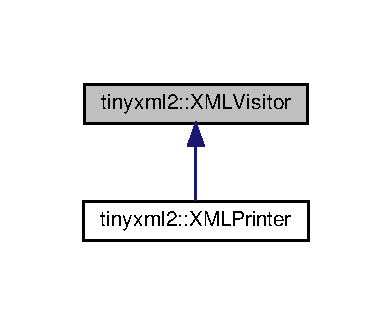
\includegraphics[width=188pt]{classtinyxml2_1_1_x_m_l_visitor__inherit__graph}
\end{center}
\end{figure}
\subsection*{Public Member Functions}
\begin{DoxyCompactItemize}
\item 
\mbox{\Hypertarget{classtinyxml2_1_1_x_m_l_visitor_acb3c22fc5f60eb9db98f533f2761f67d}\label{classtinyxml2_1_1_x_m_l_visitor_acb3c22fc5f60eb9db98f533f2761f67d}} 
virtual bool \hyperlink{classtinyxml2_1_1_x_m_l_visitor_acb3c22fc5f60eb9db98f533f2761f67d}{Visit\+Enter} (const \hyperlink{classtinyxml2_1_1_x_m_l_document}{X\+M\+L\+Document} \&)
\begin{DoxyCompactList}\small\item\em Visit a document. \end{DoxyCompactList}\item 
\mbox{\Hypertarget{classtinyxml2_1_1_x_m_l_visitor_a170e9989cd046ba904f302d087e07086}\label{classtinyxml2_1_1_x_m_l_visitor_a170e9989cd046ba904f302d087e07086}} 
virtual bool \hyperlink{classtinyxml2_1_1_x_m_l_visitor_a170e9989cd046ba904f302d087e07086}{Visit\+Exit} (const \hyperlink{classtinyxml2_1_1_x_m_l_document}{X\+M\+L\+Document} \&)
\begin{DoxyCompactList}\small\item\em Visit a document. \end{DoxyCompactList}\item 
\mbox{\Hypertarget{classtinyxml2_1_1_x_m_l_visitor_af97980a17dd4e37448b181f5ddfa92b5}\label{classtinyxml2_1_1_x_m_l_visitor_af97980a17dd4e37448b181f5ddfa92b5}} 
virtual bool \hyperlink{classtinyxml2_1_1_x_m_l_visitor_af97980a17dd4e37448b181f5ddfa92b5}{Visit\+Enter} (const \hyperlink{classtinyxml2_1_1_x_m_l_element}{X\+M\+L\+Element} \&, const \hyperlink{classtinyxml2_1_1_x_m_l_attribute}{X\+M\+L\+Attribute} $\ast$)
\begin{DoxyCompactList}\small\item\em Visit an element. \end{DoxyCompactList}\item 
\mbox{\Hypertarget{classtinyxml2_1_1_x_m_l_visitor_a772f10ddc83f881956d32628faa16eb6}\label{classtinyxml2_1_1_x_m_l_visitor_a772f10ddc83f881956d32628faa16eb6}} 
virtual bool \hyperlink{classtinyxml2_1_1_x_m_l_visitor_a772f10ddc83f881956d32628faa16eb6}{Visit\+Exit} (const \hyperlink{classtinyxml2_1_1_x_m_l_element}{X\+M\+L\+Element} \&)
\begin{DoxyCompactList}\small\item\em Visit an element. \end{DoxyCompactList}\item 
\mbox{\Hypertarget{classtinyxml2_1_1_x_m_l_visitor_adc75bd459fc7ba8223b50f0616767f9a}\label{classtinyxml2_1_1_x_m_l_visitor_adc75bd459fc7ba8223b50f0616767f9a}} 
virtual bool \hyperlink{classtinyxml2_1_1_x_m_l_visitor_adc75bd459fc7ba8223b50f0616767f9a}{Visit} (const \hyperlink{classtinyxml2_1_1_x_m_l_declaration}{X\+M\+L\+Declaration} \&)
\begin{DoxyCompactList}\small\item\em Visit a declaration. \end{DoxyCompactList}\item 
\mbox{\Hypertarget{classtinyxml2_1_1_x_m_l_visitor_af30233565856480ea48b6fa0d6dec65b}\label{classtinyxml2_1_1_x_m_l_visitor_af30233565856480ea48b6fa0d6dec65b}} 
virtual bool \hyperlink{classtinyxml2_1_1_x_m_l_visitor_af30233565856480ea48b6fa0d6dec65b}{Visit} (const \hyperlink{classtinyxml2_1_1_x_m_l_text}{X\+M\+L\+Text} \&)
\begin{DoxyCompactList}\small\item\em Visit a text node. \end{DoxyCompactList}\item 
\mbox{\Hypertarget{classtinyxml2_1_1_x_m_l_visitor_acc8147fb5a85f6c65721654e427752d7}\label{classtinyxml2_1_1_x_m_l_visitor_acc8147fb5a85f6c65721654e427752d7}} 
virtual bool \hyperlink{classtinyxml2_1_1_x_m_l_visitor_acc8147fb5a85f6c65721654e427752d7}{Visit} (const \hyperlink{classtinyxml2_1_1_x_m_l_comment}{X\+M\+L\+Comment} \&)
\begin{DoxyCompactList}\small\item\em Visit a comment node. \end{DoxyCompactList}\item 
\mbox{\Hypertarget{classtinyxml2_1_1_x_m_l_visitor_a14e4748387c34bf53d24e8119bb1f292}\label{classtinyxml2_1_1_x_m_l_visitor_a14e4748387c34bf53d24e8119bb1f292}} 
virtual bool \hyperlink{classtinyxml2_1_1_x_m_l_visitor_a14e4748387c34bf53d24e8119bb1f292}{Visit} (const \hyperlink{classtinyxml2_1_1_x_m_l_unknown}{X\+M\+L\+Unknown} \&)
\begin{DoxyCompactList}\small\item\em Visit an unknown node. \end{DoxyCompactList}\end{DoxyCompactItemize}


\subsection{Detailed Description}
Implements the interface to the \char`\"{}\+Visitor pattern\char`\"{} (see the Accept() method.) If you call the Accept() method, it requires being passed a \hyperlink{classtinyxml2_1_1_x_m_l_visitor}{X\+M\+L\+Visitor} class to handle callbacks. For nodes that contain other nodes (Document, Element) you will get called with a Visit\+Enter/\+Visit\+Exit pair. Nodes that are always leafs are simply called with \hyperlink{classtinyxml2_1_1_x_m_l_visitor_adc75bd459fc7ba8223b50f0616767f9a}{Visit()}.

If you return \textquotesingle{}true\textquotesingle{} from a Visit method, recursive parsing will continue. If you return false, {\bfseries no children of this node or its siblings} will be visited.

All flavors of Visit methods have a default implementation that returns \textquotesingle{}true\textquotesingle{} (continue visiting). You need to only override methods that are interesting to you.

Generally Accept() is called on the \hyperlink{classtinyxml2_1_1_x_m_l_document}{X\+M\+L\+Document}, although all nodes support visiting.

You should never change the document from a callback.

\begin{DoxySeeAlso}{See also}
\hyperlink{classtinyxml2_1_1_x_m_l_node_a81e66df0a44c67a7af17f3b77a152785}{X\+M\+L\+Node\+::\+Accept()} 
\end{DoxySeeAlso}


The documentation for this class was generated from the following file\+:\begin{DoxyCompactItemize}
\item 
/home/ijlee/workspace/sdmt/src/tinyxml2.\+h\end{DoxyCompactItemize}

%--- End generated contents ---

% Index
\backmatter
\newpage
\phantomsection
\clearemptydoublepage
\addcontentsline{toc}{chapter}{Index}
\printindex

\end{document}
